\mbox{}\vfill\normalsize\thispagestyle{empty}
\noindent{}\textit{Ao meu filho\\[-5pt]
Nikita Alekséievitch Tolstói,\\[-5pt]
com grande estima.\\[-5pt]
O Autor}

\chapter{Manhã ensolarada}\label{texto}

Nikita deu um suspiro ao despertar e abriu os olhos. O sol brilhava
através das ramagens de gelo nas janelas, através das estrelas
maravilhosamente prateadas e dos galhos em forma de garras. A luz no
quarto era de um branco nevado. Uma nesga de sol, batendo na tina do
lavatório, refletia"-se tremulando na parede.

Abrindo os olhos, Nikita lembrou que na noite anterior o carpinteiro
Pakhom dissera a ele:

--- Vou untá"-lo com óleo e derramar água, e de manhã, quando você se
levantar, será sentar e voar.

Na véspera, ao anoitecer, Pakhom, um mujique\footnote{Mujique, campônio russo, assim designado principalmente antes de 1917.} caolho e bexiguento,
construíra para Nikita, conforme seu pedido especial, um trenó do tipo
banquinho. Assim fizera:

Na bancada da cocheira, no meio de aparas perfumadas de madeira torcidas
em anéis, Pakhom havia aplainado duas tábuas e quatro pezinhos; a parte da
frente da tábua de baixo --- o nariz --- fora chanfrada, para que não
emperrasse na neve; os pezinhos torneados; na tábua de cima foram
feitos dois recortes para os pés, para que ficasse mais jeitoso sentar.
A tábua de baixo fora besuntada com esterco de vaca e regada três vezes
com água, sob frio intenso, e depois disso ficara como um espelho; por
fim à tábua de cima fora amarrada uma cordinha para puxar o trenó e para
conduzi"-lo na descida de morros.

A essa altura, naturalmente, o trenó já estava pronto junto à escadaria
da entrada. Pakhom era um homem assim: ``Quando eu prometo uma coisa, é
lei, farei sem falta'', repetia ele.

Nikita sentou"-se na beira da cama e aguçou o ouvido --- a casa estava em
silêncio, provavelmente ainda ninguém havia se levantado. Se ele se
vestisse num minutinho, claro que sem lavagem de mãos e rosto nem
escovação de dentes, seria possível sair correndo para o quintal pela
entrada de serviço. E do quintal ir para o rio. Lá, nas margens
íngremes, o vento havia juntado muita neve --- era sentar no trenó e
voar.

Nikita levantou"-se da cama e, na ponta dos pés, passou sobre os
quadrados quentes e ensolarados do chão\ldots{}

Nesse instante, a porta se entreabriu e no quarto se enfiou uma cabeça
de óculos, sobrancelhas ruivas espetadas e barba de um ruivo"-vivo. A
cabeça piscou e disse:

--- Não vai levantar, gaiato?

\begin{figure}
\vspace*{-2.65cm}
\hspace*{-3.25cm}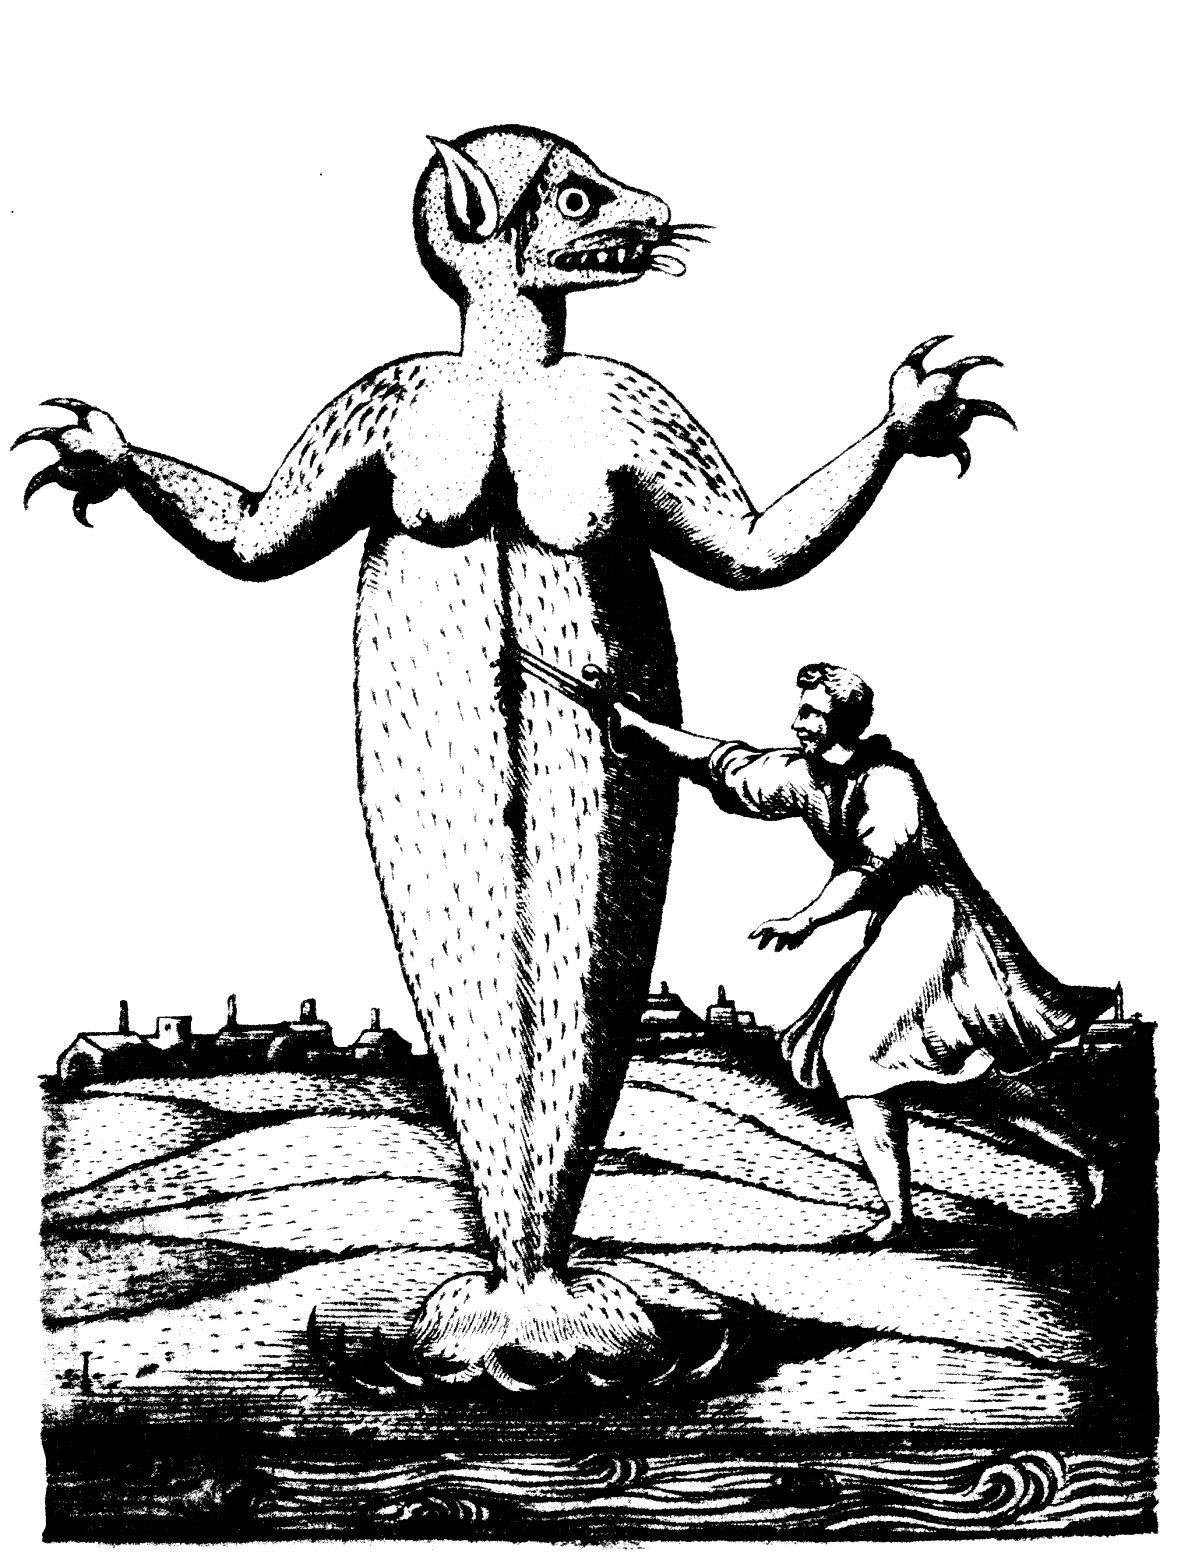
\includegraphics[width=155mm]{./imgs/1.pdf}
\end{figure}

\chapter{Arkádi Ivánovitch}

O homem de barba ruiva --- Arkádi Ivánovitch, o preceptor de Nikita ---
farejara tudo ainda na véspera e se levantara mais cedo de caso pensado.
Um sujeito surpreendentemente desenvolto e esperto era esse Arkádi
Ivánovitch. Entrou no quarto de Nikita sorrindo, parou perto da janela,
bafejou o vidro e, quando este ficou transparente, ajeitou os óculos e
olhou para o quintal.

--- Há um trenó magnífico --- disse ele --- perto da entrada.

Nikita ficou calado e franziu o cenho. Foi obrigado a se vestir e a
escovar os dentes, e a lavar não apenas as mãos, mas também as orelhas e
o pescoço. Em seguida, Arkádi Ivánovitch enlaçou Nikita pelos ombros e o
levou até a sala de jantar. À mesa provida de um samovar,\footnote{\textls[-15]{Samovar, utensílio tradicional russo usado para ferver a água do chá.}} estava sentada
sua mãezinha com um vestido cinza quente. Ela tomou o rosto de Nikita
nas mãos, fixou seus olhos claros nos dele e o beijou.

--- Dormiu bem, Nikita?

Depois, estendeu a mão a Arkádi Ivánovitch e perguntou com ternura:

--- E o senhor, Arkádi Ivánovitch, como dormiu?

--- Dormir, até que eu dormi bem --- respondeu ele, sorrindo não se sabia
de que atrás dos bigodes ruivos, então sentou"-se à mesa, verteu nata no chá,
jogou um torrãozinho de açúcar na boca, apanhando"-o com os dentes brancos,
e piscou para Nikita por detrás dos óculos.

Arkádi Ivánovitch era um homem insuportável: sempre se divertia, sempre
piscava, não dizia nada diretamente, mas de um jeito que afligia o
coração. Por exemplo, aparentemente, a mãezinha tinha perguntado com
clareza: ``Como o senhor dormiu?''. Ele respondeu: ``Dormir, até que eu
dormi bem'', e isso devia ser entendido assim: ``Já Nikita, ele queria
correr para o rio sem tomar chá e sem ter aulas, e ontem, em vez de
traduzir do alemão, ficou duas horas sentado na bancada do Pakhom''.

Arkádi Ivánovitch, verdade seja dita, nunca se queixava de Nikita, em
compensação este precisava ficar de orelha em pé o tempo todo.

Durante o chá, a mãezinha disse que à noite fizera um frio congelante,
no corredor da entrada a água da tina até congelara, e que, quando
fossem sair a passeio, Nikita precisaria colocar o
\emph{bachlyk.}\footnote{Colocado sobre o chapéu, o \emph{bachlyk} é uma
  espécie de capuz com longas abas que são enroladas no pescoço.}

--- Mamãe, palavra, está fazendo um calor de rachar --- disse Nikita.

--- Peço que coloque o \emph{bachlyk}.

--- Ele pinica e sufoca, mamãe; ficarei ainda mais resfriado com esse
\emph{bachlyk}.

A mãezinha olhou em silêncio para Arkádi Ivánovitch e para Nikita e,
quando falou, sua voz estremeceu:

--- Eu não sei a quem você puxou de tão desobediente.

--- Vamos estudar --- disse Arkádi Ivánovitch, levantando"-se
decididamente e esfregando as mãos com rapidez, como se neste mundo não
houvesse prazer maior do que resolver questões aritméticas e ditar
provérbios e refrões de dar sono.

Em um quarto branco, grande e vazio, em cuja parede estava pendurado o
mapa de dois hemisférios, Nikita sentou"-se a uma mesa toda manchada de
tinta e com carinhas desenhadas. Arkádi Ivánovitch abriu o livro de
exercícios.

--- Pois bem --- disse energicamente ---, onde paramos?

E, com um lápis apontado, sublinhou o número da questão.

``Um lojista vendeu alguns \emph{archins}\footnote{\emph{Archin,} antiga
  medida russa de comprimento equivalente a 0,71m.} de tecido azul a 3
rublos e 64 copeques o \emph{archin}, e de tecido preto a\ldots{}'' --- leu
Nikita. Imediatamente, como costumava acontecer, aquele lojista do livro
de exercícios surgiu"-lhe na imaginação. Estava de sobrecasaca comprida e
empoeirada, o rosto amarelo e desanimado, uma figura enfadonha, achatada e
magra. Sua lojinha era escura, como uma fenda; numa prateleira
empoeirada se achavam duas peças de tecido --- o lojista esticava as mãos
magras, tirava as peças da prateleira e fitava Nikita com olhos opacos e
sem vida.

--- Então, o que você acha, Nikita? --- perguntou Arkádi Ivánovitch. ---
O lojista vendeu 18 \emph{archins}. Quanto foi vendido de tecido azul e
quanto de tecido preto?

Nikita franziu o cenho, o lojista ficou completamente achatado, as duas
peças de tecido se enfiaram na parede e cobriram"-se de poeira\ldots{} 

Arkádi Ivánovitch disse: ``Ai, ai!'' --- e começou a explicar, escreveu
rapidamente números para multiplicar e dividir, repetindo: ``Sobe o 1,
sobe o 2''. Nikita tinha a impressão de que, durante a multiplicação, o
1 e o 2 saltavam do papel para dentro de sua cabeça e lá faziam cócegas
até que fossem esquecidos. Isso era muito maçante. No quarto de estudar,
o sol faiscava em duas janelas cobertas de geada e o seduzia: ``Vamos ao
rio\ldots{}''.

Finalmente a aritmética terminou e começou o ditado. Arkádi Ivánovitch
passou a andar ao longo das paredes e com voz especialmente sonolenta,
com a qual as pessoas de verdade não falam, ditava:

``\ldots{}Todos os animais que existem na Terra se esforçam continuamente,
trabalham. O aluno era obediente e aplicado\ldots{}''.

Colocando a pontinha da língua para fora, Nikita escrevia e a pena
rangia e respingava.

De repente, dentro de casa, a porta bateu e ouviram"-se pelo corredor
passos de botas de feltro cobertas de gelo. Arkádi Ivánovitch baixou o
livro e prestou atenção. A voz alegre da mãezinha soou alto por perto:

--- O que foi, trouxeram a correspondência?

Nikita deitou totalmente a cabeça sobre o caderno --- tamanha era a
vontade de rir.

--- Obediente e aplicado --- repetia cantarolando ---, ``aplicado'' eu
escrevi.

Arkádi Ivánovitch ajeitou os óculos.

--- Em suma, todos os animais que existem na Terra são obedientes e
aplicados\ldots{} Por que você está rindo?\ldots{} Fez um borrão?\ldots{} Aliás, agora
vamos fazer um intervalo.

Arkádi Ivánovitch apertou os lábios, ameaçou"-o com o dedo comprido como
um lápis e saiu rapidamente do quarto. No corredor, perguntou à
mãezinha:

--- Aleksandra Leóntievna, será que não tem uma cartinha para mim?

Nikita compreendeu de quem ele estava esperando uma carta. Mas não tinha
tempo a perder. Vestiu uma peliça curta e botas de feltro, enfiou o
\emph{bachlyk} debaixo da cômoda para que não o achassem e correu até a
entrada de casa.

\chapter{Montes de neve}

O amplo quintal estava repleto de neve brilhante, branca e macia. Nela
havia as pegadas profundas e azuladas das pessoas e os rastos juntinhos
dos cachorros. O ar frio e penetrante beliscava o nariz e pinicava as
bochechas como agulhas. A cocheira, os galpões e os currais, cobertos de
chapéus brancos, encolheram, como se tivessem crescido ao contrário na
neve. Os trilhos deixados pelos patins do trenó corriam como tiras de
vidro por todo o quintal.

Nikita desceu a toda pela escadaria da entrada, fazendo os degraus
estalarem. Embaixo estava o trenó novinho feito de abeto, com uma corda
amarrada. Nikita o vistoriou --- era bem feito ---, experimentou ---
deslizava bem ---, então carregou"-o sobre o ombro, apanhou uma pequena
pá para qualquer eventualidade, e correu até o dique pela estrada em
frente ao jardim. No dique havia salgueiros largos, gigantescos, que
chegavam quase até o céu; estavam agora cobertos de gelo e cada galhinho
parecia feito de neve.

Nikita virou à direita, na direção do rio, e se esforçou para se manter
na estrada, pisando nas pegadas que outros deixaram; já nos lugares onde
a neve estava intocada e limpa, ele andava de costas para despistar
Arkádi Ivánovitch.

Nas margens íngremes do rio Tchagrá\footnote{Tchagrá, rio afluente do
  Volga na região de Samara.} o vento acumulara grandes amontoados de
neve fofa durante os últimos dias. Em alguns lugares esses montes
prendiam"-se ao riozinho, formando uma espécie de beiral. Bastava alguém
se postar sobre um beiral para que este desmoronasse, desaparecesse, e uma
montanha de neve rolava para baixo envolta em uma nuvem de poeira branca.

À direita, o riacho ziguezagueava como uma sombra azulada entre os
campos brancos e desertos. À esquerda, sobre uma escarpa, isbás\footnote{Isbá, casa de camponês na Rússia, tradicionalmente feita de troncos.}
pretejavam e as varas dos poços da aldeia Sosnovka espetavam"-se entre
elas. Fumaças azuis subiam sobre os telhados e se desfaziam. Num
penhasco nevado, onde havia manchas e faixas amarelas das cinzas que as
donas de casa tinham retirado de suas estufas\footnote{No original,
  \emph{pietchka}, que pode ser constituída de uma grande estrutura com
  lareira e fogão embutido. Em cima dela, numa espécie de patamar,
  costumava"-se dormir em dias frios.} nessa manhã, figuras minúsculas se
moviam. Eram os amigos de Nikita, os garotos do ``nosso lado'' da
aldeia. E adiante, onde o rio fazia a curva, viam"-se contornos dе outros
garotos, os ``do outro lado'', todos muito perigosos. Largando a pá, Nikita
pôs o trenó"-banquinho na neve, sentou nele, agarrou fortemente a
corda e empurrou o chão com os pés umas duas vezes, então o trenó começou a
deslizar sozinho pelo morro. O vento assobiava nos ouvidos, dos dois
lados levantou"-se uma poeira de neve. Para baixo, sempre para baixo, Nikita
ia como uma flecha. Lá onde a neve terminava, o trenó passou voando pela
escarpa e deslizou sobre o gelo. Foi desacelerando, desacelerando e
parou.

Nikita começou a rir, levantou"-se do trenó e o puxou para cima do morro,
atolando na neve. Enquanto subia a margem, não muito longe, num campo
nevado, viu uma figura preta, de estatura acima de um homem normal, que
parecia Arkádi Ivánovitch. Nikita pegou sua pazinha, jogou"-se no trenó e
deslizou para baixo, indo para onde os montes de neve se prendiam ao rio
como beirais.

Colocando"-se bem debaixo de um beiral, Nikita começou a cavar
uma gruta. O trabalho era fácil --- trinchar neve com a pá. Terminando
de cavar a gruta, ele se enfiou nela, puxou o trenó e começou a
fechar o orifício por dentro com bolas de neve. Quando acabou de erguer
a parede branca, dentro se difundiu uma meia luz azul e ficou
aconchegante e agradável.

Nikita estava sentado imaginando que nenhum dos garotos tinha um trenó
tão maravilhoso como aquele. Ele tirou o canivete e começou a esculpir
na tábua de cima o nome ``Vevit''.

--- Nikita! Onde você se meteu? --- ele ouviu a voz de Arkádi
Ivánovitch.

Nikita colocou o canivete no bolso e olhou por uma fresta entre as bolas
de neve. Embaixo, no gelo, postava"-se Arkádi Ivánovitch, com a cabeça
erguida.

--- Onde está você, gaiato?

Arkádi Ivánovitch ajeitou os óculos e começou a subir na gruta, mas logo
afundou na neve até a cintura.

--- Saia sozinho, pois vou tirar você daí de qualquer jeito.

Nikita ficou em silêncio. Arkádi Ivánovitch tentou subir mais um pouco,
mas atolou de novo, enfiou as mãos nos bolsos e disse:

--- Não quer, então não precisa. Pode ficar aí. É que sua mãe recebeu
uma carta de Samara\ldots{} Porém, adeus, estou indo embora\ldots{}

--- Que carta? --- perguntou Nikita

--- A"-há! Então você está aí mesmo.

--- Diga lá, de quem é a carta?

--- É uma carta sobre a visita de certas pessoas para as festas.

No ato começaram a rolar bolas de neve. E, na gruta, surgiu a cabeça de
Nikita. Arkádi Ivánovitch riu alegremente.

\chapter{A carta misteriosa}

Durante o almoço, a mãezinha finalmente leu a carta. Era do pai:

--- ``Querida Sacha,\footnote{Sacha é apelido de Aleksandra.} eu comprei
o que nós tínhamos resolvido dar a certo menino que, a meu ver,
dificilmente merece um presente maravilhoso desses'' --- ao ouvir essas
palavras, Arkádi Ivánovitch começou a piscar terrivelmente. --- ``Esse
presente é bastante grande, por isso mande uma carroça separada para
buscá"-lo. E mais uma novidade: Anna Apollóssovna Bábkina pretende nos
visitar nas festas natalinas em companhia das crianças\ldots{}''.

--- E o resto não interessa --- disse a mãezinha, e a todas as perguntas
de Nikita somente fechava os olhos e abanava a cabeça: --- Não sei de
nada.

Arkádi Ivánovitch também estava em silêncio e, abrindo os braços, dizia:
``Não sei de nada''. E, em geral, estava muito alegre, respondia fora de
propósito e, vez ou outra, também tirava do bolso uma cartinha, lia duas
linhas e apertava os lábios. Pelo visto, ele também tinha um segredo.

Ao escurecer, Nikita correu pelo quintal para a ala dos criados, de onde
a luz de duas janelinhas cobertas de gelo incidia sobre a neve lilás. Na
ala dos criados estavam jantando. Nikita assobiou três vezes. Minutos
depois, apareceu seu melhor amigo, Michka Koriachónok, calçando umas
botas de feltro enormes, sem chapéu e com uma peliça curta jogada sobre
os ombros. Lá mesmo, ao virar a esquina, Nikita, sussurrando, contou da
carta e perguntou o que trariam da cidade.

Michka Koriachónok, batendo os dentes de frio, disse:

--- Na certa alguma coisa enorme, que um raio caia na minha cabeça se
não for isso. Vou dar no pé, está frio. Escute, amanhã lá na aldeia nós queremos
bater nos garotos do outro lado. Você vai também?

--- Está bem.

Nikita voltou para casa e sentou"-se para ler \emph{O cavaleiro sem
cabeça}.\footnote{\emph{O cavaleiro sem cabeça} (1886)\emph{,} romance
  de Mayne Reid (1818--1883) baseado nessa lenda medieval.}

Em volta de uma mesa redonda, sob uma grande lâmpada, estavam sentados a
mãezinha e Arkádi Ivánovitch, com livros nas mãos. Atrás da grande
estufa um grilo serrava madeira --- tr"-tr, tr"-tr. No quarto vizinho,
escuro, uma tábua do assoalho estalou.

O cavaleiro sem cabeça corria pelas pradarias, chicoteando o capim alto;
a lua vermelha se erguia sobre o lago. Nikita sentia os pelos de sua
nuca arrepiarem. Virou"-se cuidadosamente, e do outro lado das janelas
escuras passou uma sombra cinzenta. Palavra, ele a viu. Levantando a
cabeça do livro, a mãezinha disse:

--- À noite começou a ventar, teremos tempestade de neve.

\chapter{O sonho}

Nikita teve um sonho --- já o sonhara algumas vezes e era sempre o
mesmo.

A porta da sala se abriu fácil e silenciosamente. No assoalho de madeira
jaziam reflexos azulados das janelas. Do outro lado das janelas
escuras pairava a lua --- uma esfera grande e iluminada. Nikita subiu na
mesa de jogo encostada na parede, entre as janelas, e viu:

Do lado oposto, numa parede branca como giz, um pêndulo redondo
balançava numa caixa de relógio bem alta, e balançava refletindo a luz
da lua. Acima do relógio, em uma moldura, estava pendurado o retrato de um
velhinho de ar severo, com um cachimbo; ao seu lado, o de uma velhinha
de touca e xale que olhava em torno apertando os lábios. Do relógio até a quina,
ao longo da parede, poltronas largas listradas estendiam os braços,
agachadas nas quatro pernas. No canto, acomodava"-se um sofá baixinho.
Sem rostos, sem olhos, suas superfícies convexas estavam viradas para a
lua, sem se mexerem.

Um gato saiu de baixo das franjas do sofá. Espreguiçou"-se, saltou no
sofá e caminhou, preto e comprido. Andava de rabo abaixado. Dali saltou
para as poltronas, andou sobre elas junto às paredes, curvou"-se, passou
sob seus braços. Quando chegou à última, pulou no assoalho e sentou
diante do relógio, de costas para as janelas. O pêndulo balançava, o
velhinho e a velhinha olhavam severamente para o gato. Então o bichano se
levantou, apoiou"-se na caixa do relógio com uma pata e com a outra
tentou parar o pêndulo. ``A caixa não tem proteção de vidro. A qualquer
momento sua pata alcançará o pêndulo.''

Ah, se pudesse gritar! Mas Nikita não conseguia mexer um dedo --- não se
movia --- e tinha medo, muito medo de que a qualquer momento acontecesse
algo terrível.

A luz da lua jazia no chão, imóvel, em quadriláteros compridos. Tudo na
sala silenciou, afundou"-se em seus pezinhos. E o gato se esticou,
abaixou a cabeça, encolheu as orelhas e alcançou o pêndulo com a pata.
Nikita sabia que, assim que sua pata tocasse no pêndulo, ele pararia e
tudo iria trincar, rachar, tinir e desaparecer como poeira, não haveria
nem sala, nem luz da lua.

O medo fazia a cabeça de Nikita tilintar, como se nela houvesse estilhaços de vidro, e seu corpo todo formigar, como que polvilhado de areia\ldots{} Reunindo todas as
forças, ele se jogou no chão com um grito desesperado. E o chão, de
repente, despencou. Nikita sentou"-se. Olhou para os lados. No quarto
havia duas janelas cobertas de gelo; através da vidraça ele podia ver uma
lua estranha, maior do que deveria ser. No chão, um penico e um par de
botas.

``Senhor, seja louvado, Senhor!'', Nikita fez o sinal da cruz
rapidamente e enfiou a cabeça embaixo do travesseiro. O travesseiro era
quente, macio, cheio de sonhos.

Mal fechou os olhos, ele se viu de novo em pé, sobre a mesa de jogo, na
mesma sala. Sob a luz da lua, o pêndulo balançava, o velhinho e a
velhinha olhavam com severidade. De novo, debaixo do sofá, surgiu a
cabeça do gato. Mas Nikita já estendera as mãos, já saltara da mesa e,
agora, meneando os pés rapidamente, parecia voar ou flutuar sobre o
piso. Sentia um prazer incomum ao sair voando pelo quarto. Quando os pés
começavam a tocar o piso, ele levantava os braços e lentamente subia até
o teto; agora fazia um voo irregular, junto à parede. Pertinho do nariz,
viu a cornija moldada de gesso em que havia uma poeira cinzenta e
agradável e cheiro de aconchego. Depois notou na parede uma fenda
familiar que lembrava o rio Volga no mapa, depois um prego velho e muito
estranho com um pedacinho de barbante rodeado de moscas mortas.

Nikita afastou"-se da parede, empurrando"-a com o pé, e passou a voar
lentamente na direção do relógio. Em cima da caixa ficava um pequeno
vaso e no fundo dele havia algo que não era possível distinguir. E, de
repente, pareceu que disseram no ouvido de Nikita: ``Pegue o que está
lá''.

Ele aproximou"-se voando do relógio e tentou enfiar a mão no vasinho. Mas
subitamente a velhinha brava destacou"-se do quadro e com as mãos magras
pegou Nikita pela cabeça. Ele se soltou, mas do outro quadro saiu o
velhinho, começou a brandir o cachimbo comprido e acertou Nikita nas
costas com tal destreza que este caiu no chão, batendo o corpo com força
e abrindo os olhos.

O sol resplandecia e faiscava através das ramagens de gelo da janela.
Perto da cama, postava"-se Arkádi Ivánovitch, que sacudia Nikita pelo
ombro e dizia:

--- Levante, levante, são nove horas.

Quando Nikita, esfregando os olhos, sentou"-se na cama, Arkádi Ivánovitch
piscou algumas vezes e esfregou as mãos com força.

--- Hoje, irmãozinho, não teremos aulas.

--- Por quê?

--- Porque o ``por quê'' termina com a letra E. Por duas semanas poderá
correr por aí até ficar com a língua de fora. Levante.

Nikita saltou da cama e começou a dançar sobre o chão aquecido:

--- Férias de Natal! --- ele tinha esquecido completamente que nesse dia 
começavam duas longas semanas felizes. Dançando diante de Arkádi
Ivánovitch, Nikita se esqueceu de algo mais: do seu sonho, do vasinho
sobre\,o relógio e da\,voz\,que\,lhe\,sussurrou\,no\,ouvido:\,``Pegue\,o\,que\,está\,lá''.

\chapter{A velha casa}

Caíram catorze dias inteiros sobre Nikita --- ele podia fazer o que
quisesse. Ficou até um pouco tedioso.

De manhã, fez uma papa de chá, leite, pão e geleia, e comeu tanto que
precisou ficar sentado e calado algum tempo. Olhando para o samovar,
surpreendeu"-se demoradamente com o reflexo do seu rosto, que era
comprido, do tamanho do samovar, um rosto monstruoso. Depois, começou a
pensar que, se pegasse uma colher de chá e a quebrasse, daria para fazer
um barquinho com um pedaço e uma cavadeira com o outro --- para cavar
alguma coisa.

``É hora de ir passear, Nikita'', disse finalmente a mãezinha.

Ele se vestiu sem pressa e, passando o dedo na parede rebocada, andou
por todo o comprido corredor, que cheirava a calor e aconchego das
estufas. À esquerda do corredor, na parte sul da casa, ficavam os
quartos de inverno, aquecidos e habitados. À direita, do lado norte,
havia cinco aposentos de verão, semivazios, com uma sala no meio. Neles
as estufas enormes revestidas de azulejos eram aquecidas somente uma vez
por semana, os lustres de cristal estavam envolvidos por gaze, e no chão
da sala havia uma montanha de maçãs --- um leve cheiro adocicado de algo
podre enchia essa parte da casa.

Nikita entreabriu com dificuldade a porta de carvalho de duas folhas e,
na ponta dos pés, andou pelos quartos desertos. Através das janelas
semiarredondadas via o jardim entulhado de neve. As árvores estavam
imóveis, com galhos brancos caídos; as moitas de lilases dos dois lados
da escada que levava à varanda curvaram"-se sob a neve. Numa clareira
havia pegadas azuis de lebres. Bem perto da janela, em um galho, estava
pousado um corvo cabeçudo que parecia o diabo. Nikita bateu com o dedo
no vidro, o corvo saltou para o lado e voou, derrubando a neve dos
galhos com as asas.

Nikita chegou até o último quarto, no canto da casa. Lá, encostados nas
paredes e cobertos de poeira, armários de vidro refletiam o
brilho de capas de livros antigos. Em cima de uma lareira de
azulejos, havia o retrato de uma dama de beleza admirável. Ela usava
um vestido longo de montaria e, na mão revestida por uma luva que se
alargava ao cobrir o braço, segurava um chicote. Parecia que ela estava
andando e se virara para fitar Nikita com um sorriso malicioso e os
olhos longos e perscrutadores.

\begin{figure}
\vspace*{-2.65cm}
\hspace*{-2.85cm}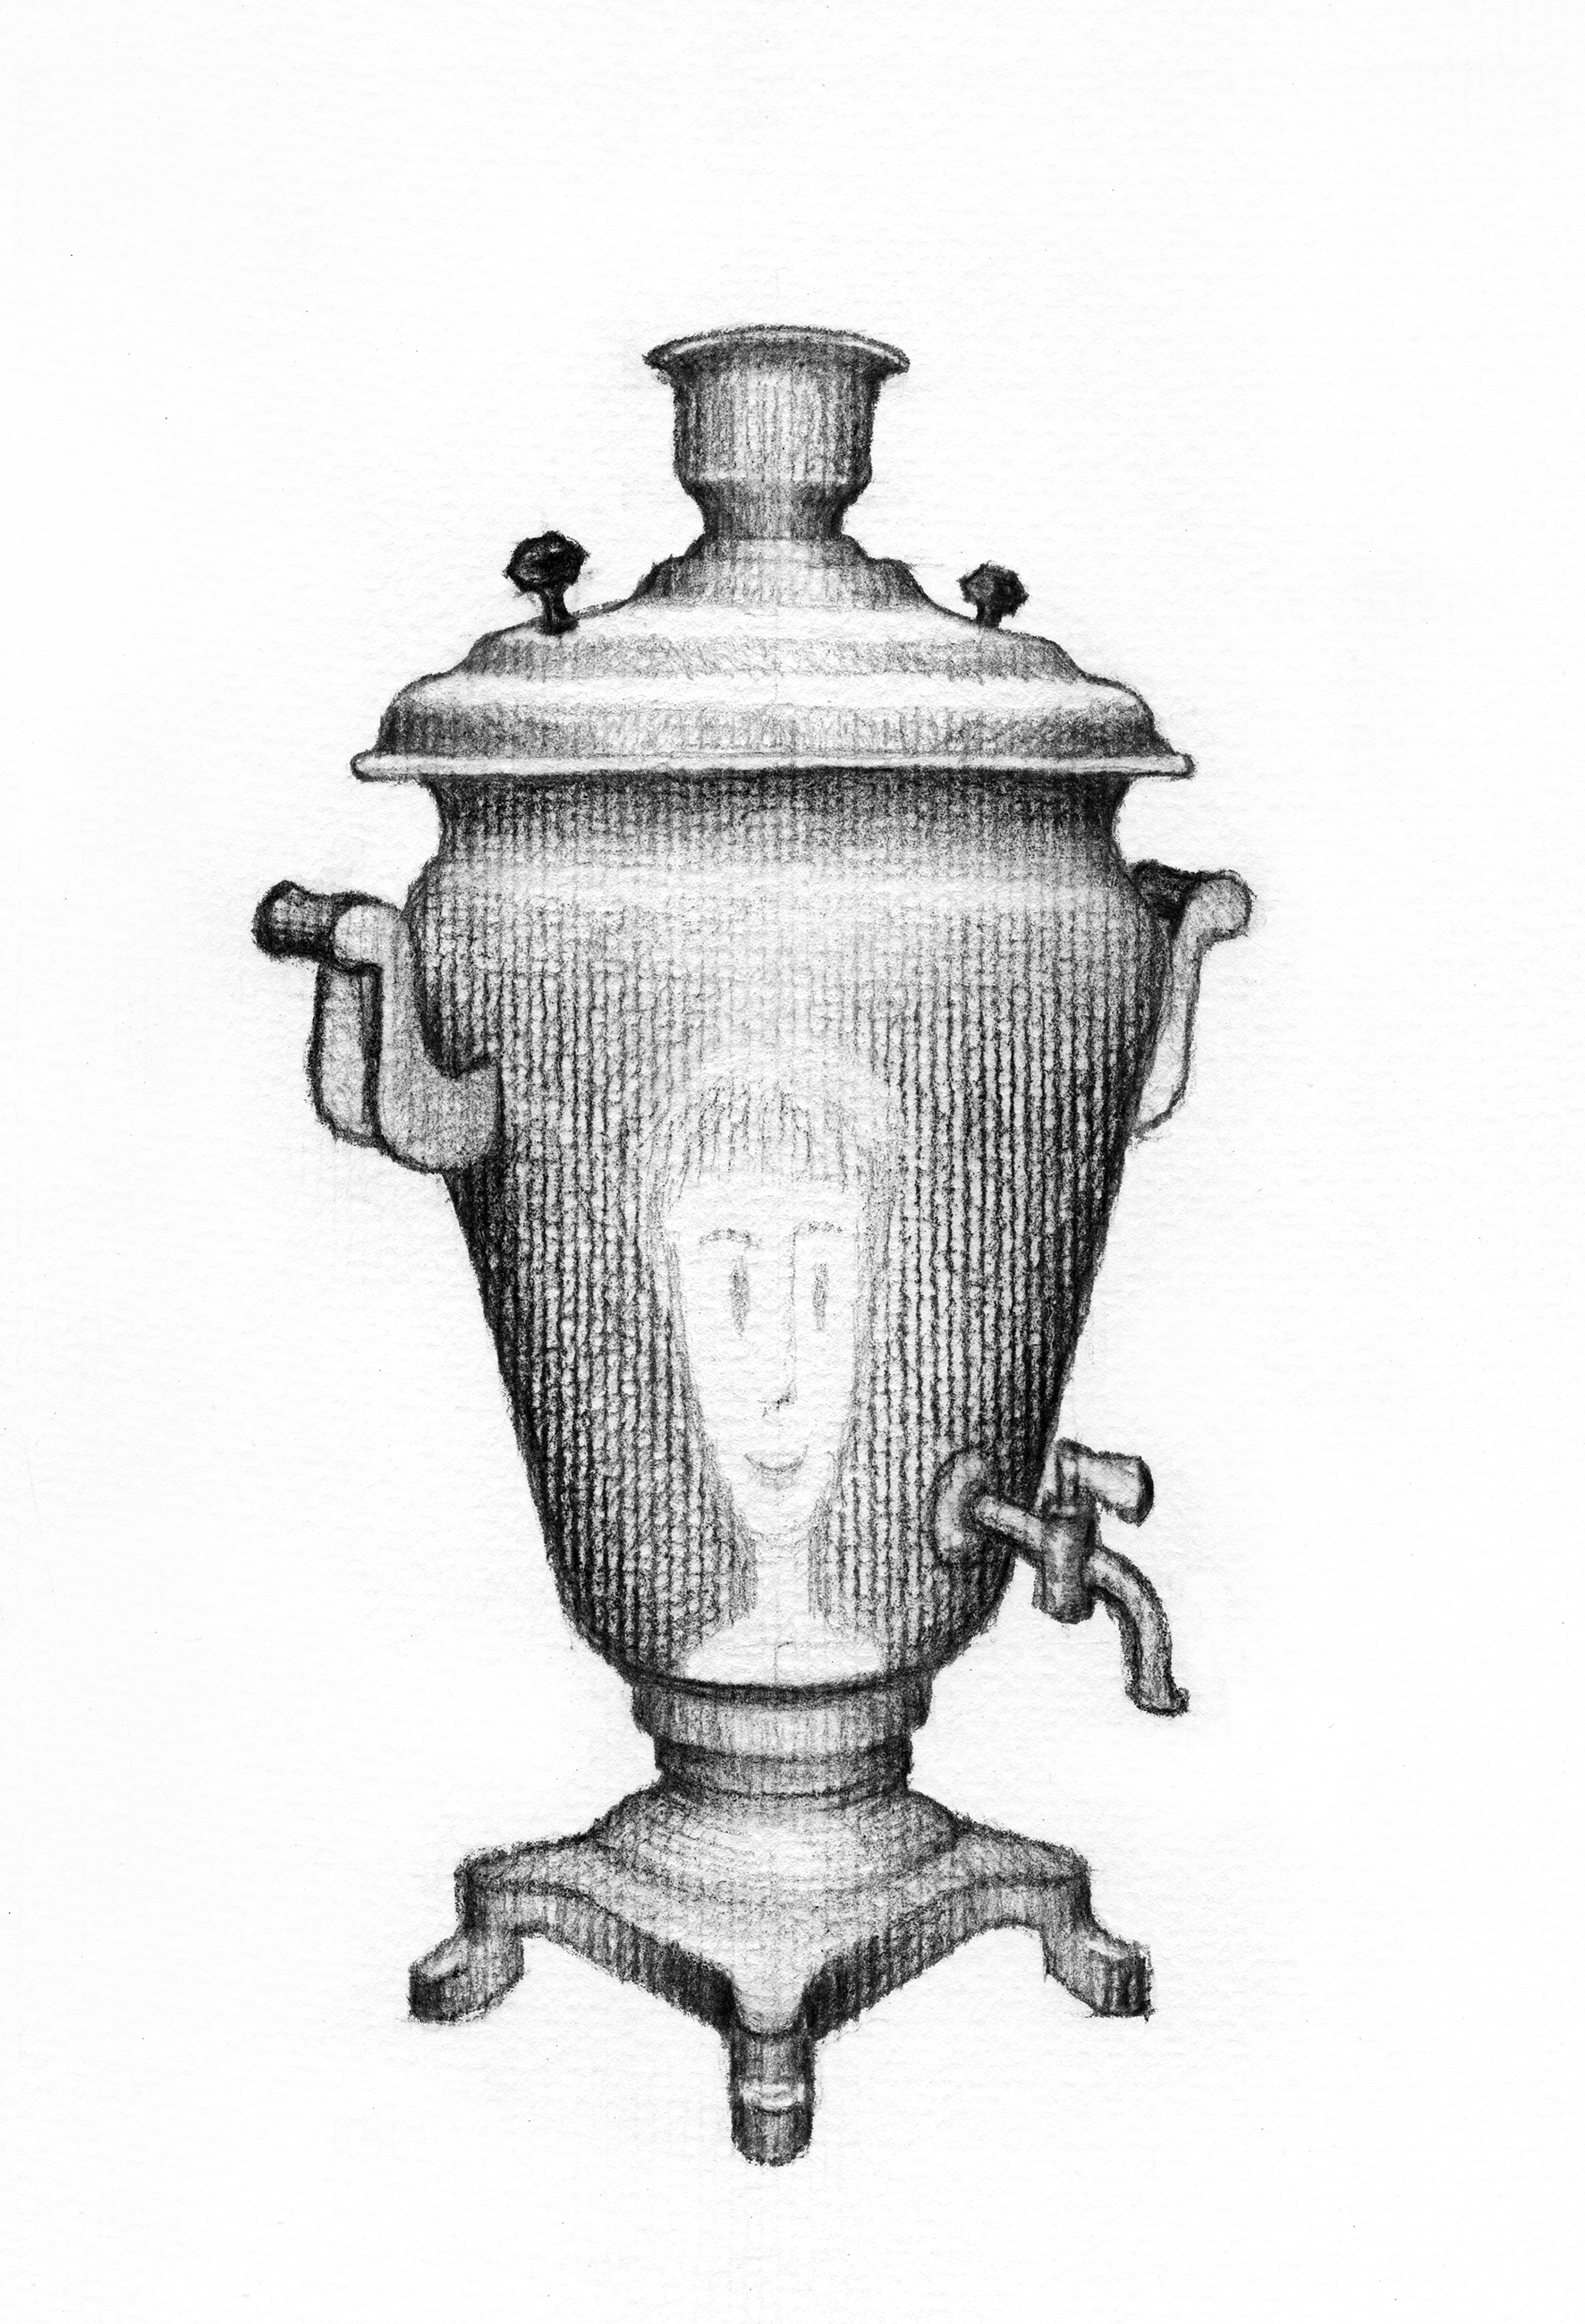
\includegraphics[width=155mm]{./imgs/3.pdf}
\end{figure}

Ele sentou"-se no sofá e, apoiando o queixo nos punhos, pôs"-se a examinar
a dama. Poderia ficar admirando"-a por muito tempo. Por causa dela ---
ouvira da mãe mais de uma vez --- grandes desgraças tinham acontecido ao
bisavô dele. O retrato do infeliz bisavô estava pendurado ali mesmo,
sobre o armário de livros --- um velho magrinho, de nariz afilado e
olhos fundos; com uma mão cheia de anéis, segurava o penhoar no peito;
ao seu lado havia um rolo de papiro semidesenrolado e uma pena de ganso.
Em tudo se via que aquele velhinho era muito infeliz.

A mãezinha contava que geralmente ele dormia de dia e à noite lia e
escrevia --- só saía para passear ao pôr do sol. De noite, vigilantes
rondavam a casa matraqueando matracas para que pássaros noturnos não
voassem sob as janelas e assustassem o bisavô. Diziam que naquele tempo o
jardim cobrira"-se de mato alto. A casa, exceto esse quarto, estava toda
fechada, inabitada. Os mujiques da criadagem fugiram. Os negócios do
bisavô chegaram a um estado absolutamente lamentável.

Uma vez, ele não fora encontrado nem no escritório, nem no resto da casa
ou no jardim --- procuraram"-no durante uma semana inteira, mas havia
simplesmente desaparecido. Cinco anos depois, um herdeiro seu recebeu
uma misteriosa carta escrita por ele na Sibéria: ``Eu procurava sossego
na sabedoria e encontrei esquecimento na natureza''.

O motivo desses estranhos acontecimentos era a dama de vestido de
montaria. Nikita olhava para ela com curiosidade e inquietação.

O corvo apareceu de novo do lado de fora, espalhou neve ao pousar num
galho, onde ficou baixando a cabeça, como se desse mergulhos, abriu o
bico e crocitou. Nikita teve uma sensação medonha. Ele deixou os quartos
desertos e correu para o quintal.

\chapter{Perto do poço}

No meio do quintal, perto do poço, onde a neve ao redor era amarela,
congelada e pisoteada, Nikita encontrou Michka Koriachónok. Ele
estava sentado na beira do poço e mergulhava na água a ponta de sua
\emph{golitsa} --- uma luva de couro inteiriça.

Nikita perguntou para que estava fazendo aquilo. Michka Koriachónok
respondeu:

--- Os garotos do outro lado molham todas as suas \emph{golitsas}, e nós
agora também vamos molhar. Elas ficam duras e podemos brigar com mais
destreza. Virá conosco para a aldeia?

--- Quando?

--- Assim que almoçarmos. Não fale nada para sua mãe.

--- Minha mãe me deixou ir, só mandou não brigar.

--- Como mandou não brigar? E se for atacado? Sabe quem vai atacar você?
Stiopka Karnaúchkin. Ele vai lhe acertar uma que derrubará você.

--- Com o Stiopka eu me resolvo --- disse Nikita ---, dou um jeito nele
com um mindinho --- е mostrou o dedo para Michka.

Koriachónok olhou, cuspiu e disse com voz grosseira:

--- Stiоpka Karnaúchkin tem um punho enfeitiçado. Na semana passada, foi
com o pai até a vila Utievka para buscar sal e peixe, e lá seu punho foi
enfeitiçado; que um raio caia sobre minha cabeça se eu estiver mentindo.

Nikita ficou pensativo --- certamente seria melhor não ir para a aldeia,
mas, se não fosse, Michka o chamaria de covarde.

--- E como enfeitiçaram o punho dele? --- perguntou.

Michka cuspiu outra vez:

--- É simples. Primeiro, pegue fuligem, passe nas mãos e fale três
vezes: ``\emph{Tani"-bani}, o que há abaixo de nós, abaixo das colunas de
ferro?''. Isso é tudo\ldots{}

Nikita olhou para Koriachónok com grande respeito. Nesse meio"-tempo, no
quintal os portões se abriram e ovelhas saíram num rebanho denso e
cinzento --- os cascos miúdos batiam como o tamborilar de dedos, os
rabinhos sacudiam e deixavam cair nozinhos de esterco. O rebanho de
ovelhas se amontoou perto do poço. Balindo e se apertando, as ovelhas se
enfiaram no cocho, quebraram o gelo fino com os focinhos, beberam água e
tossiram. Um carneiro sujo e de pelo comprido encarou Michka com os
olhos brancos manchados e bateu com a pata no chão. Michka disse a ele:
``Molenga!'' --- e o carneiro avançou contra ele, mas o menino saltou
sobre o cocho a tempo.

Nikita e Michka correram pelo quintal, rindo e zombando do carneiro. O
bicho quis ir atrás deles, mas pensou melhor e baliu, como se dissesse:

--- Vocês meeesmos é que são moooleengass.

Quando gritaram da entrada de casa para que Nikita fosse almoçar, Michka
Koriachónok disse:

--- Olhe lá, não vá me enganar, ainda vamos para a aldeia.

\begin{figure}
\vspace*{-2.65cm}
\hspace*{-2.85cm}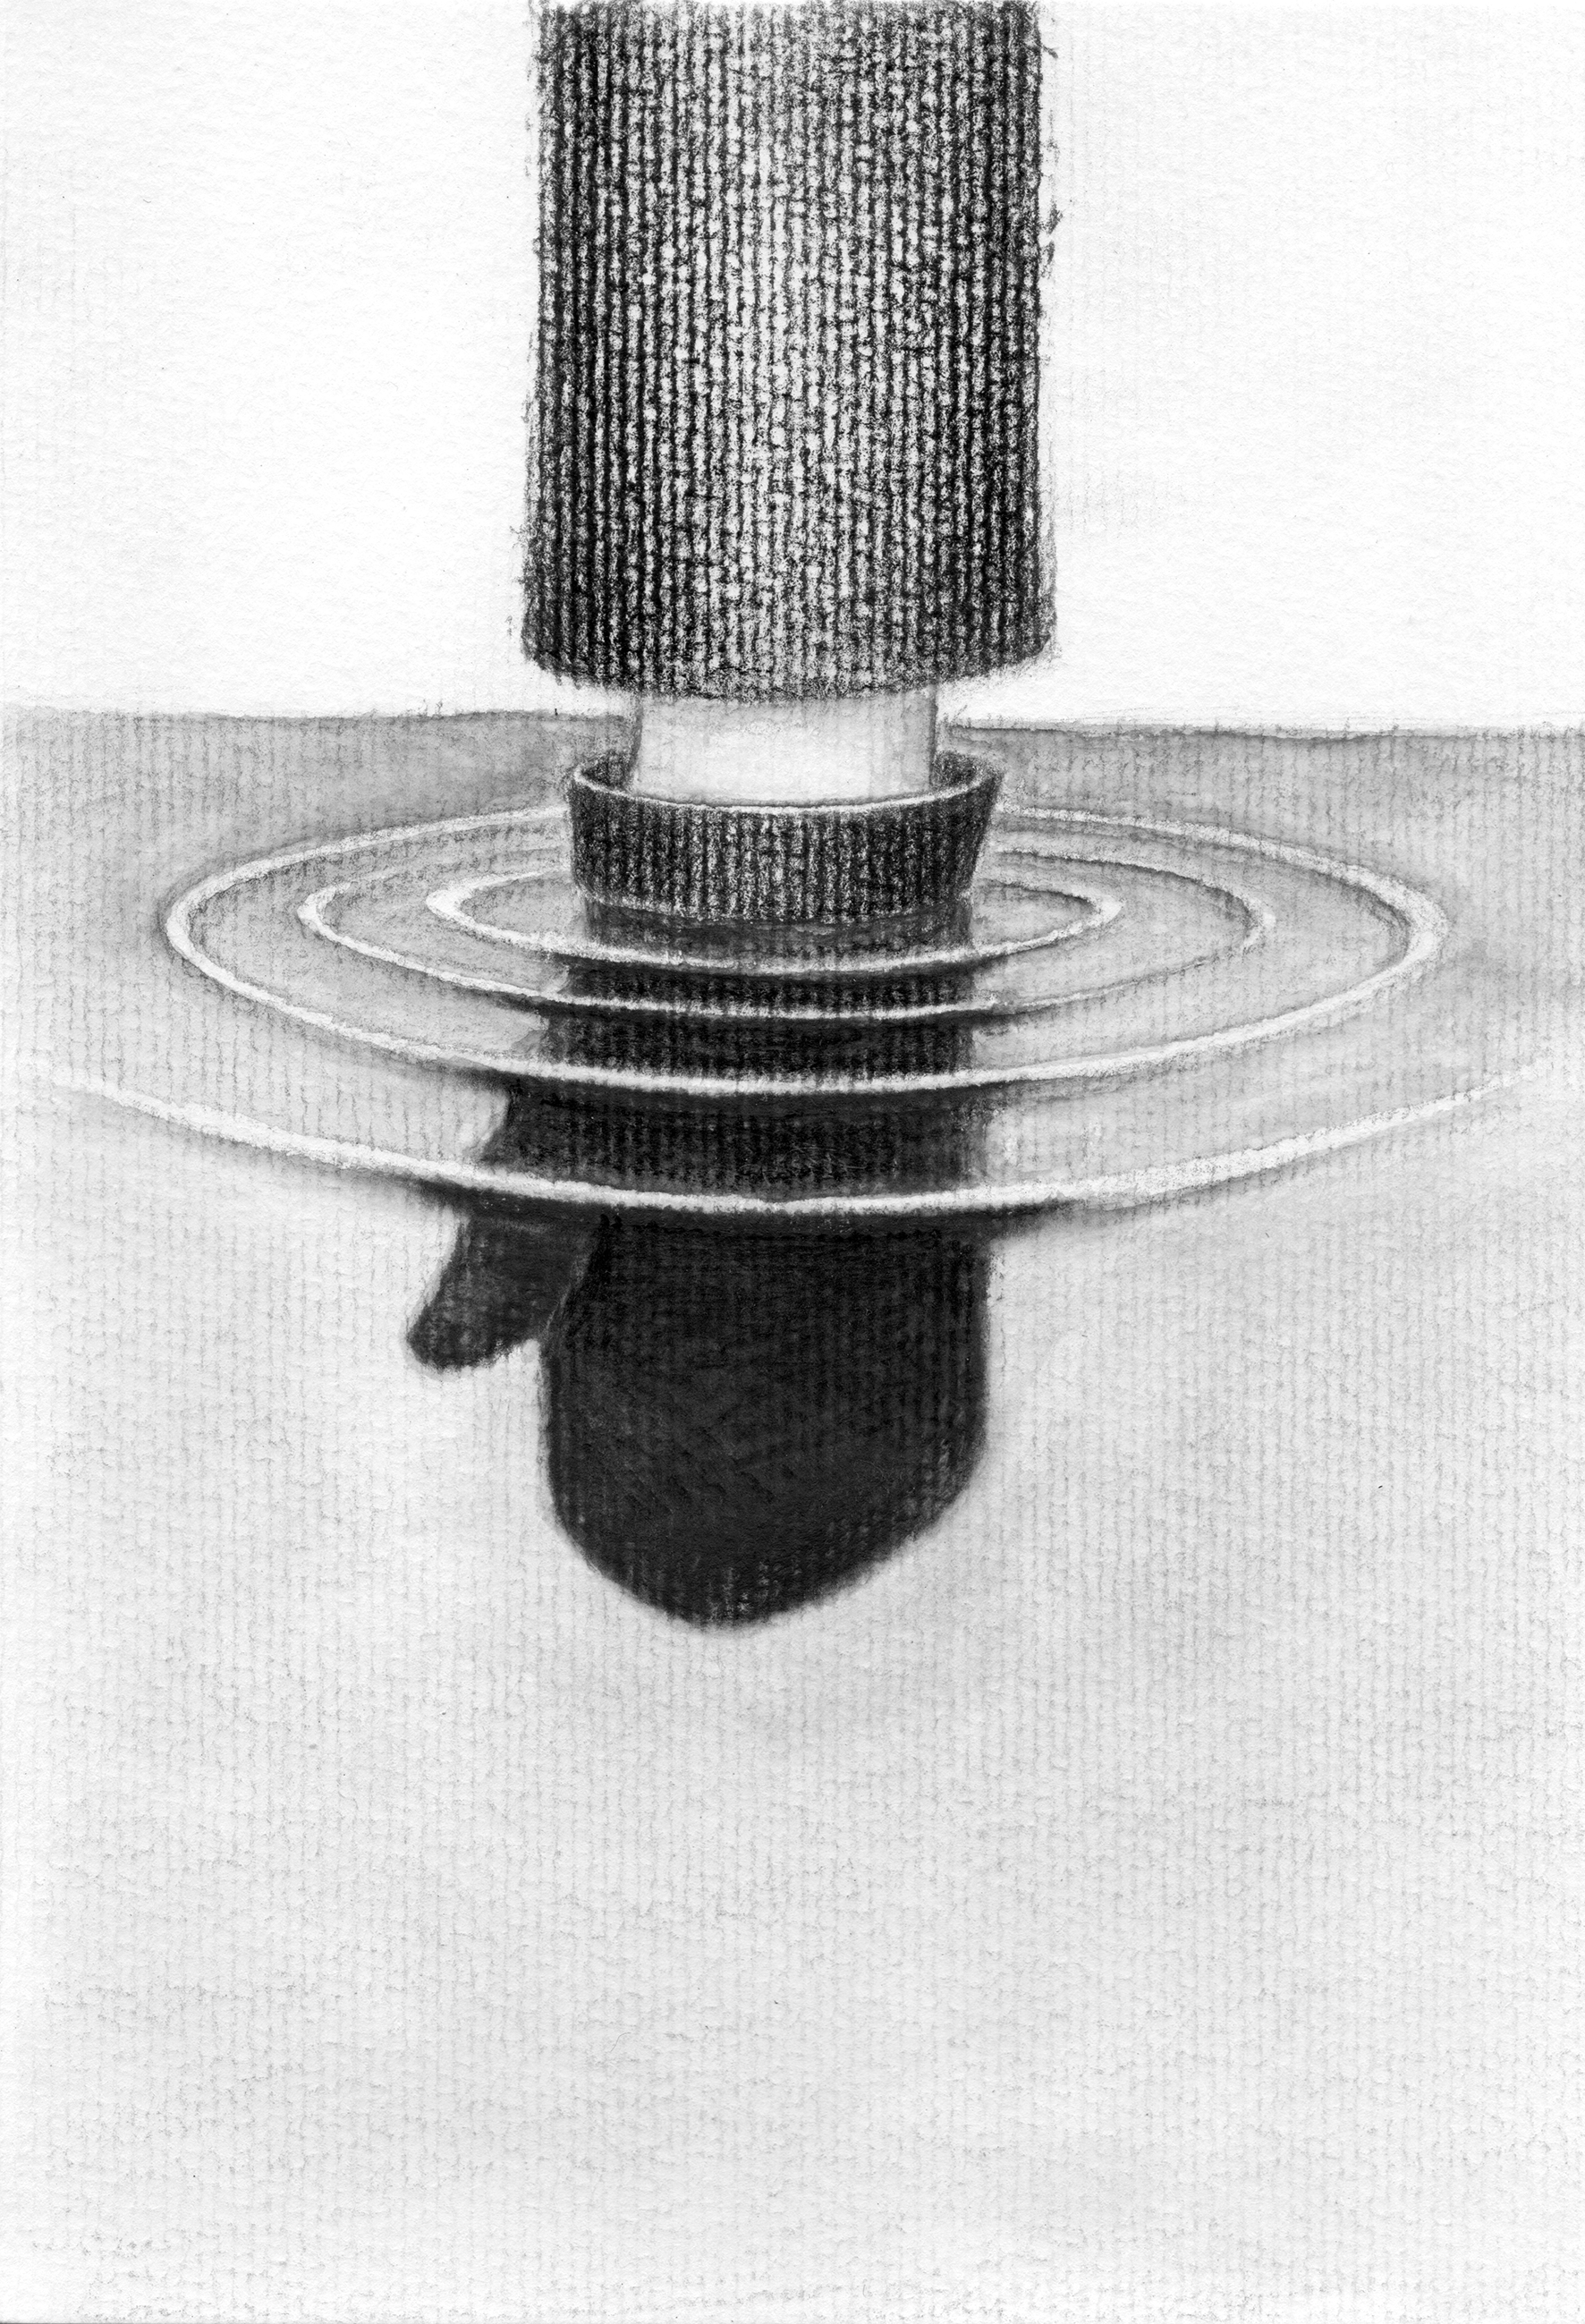
\includegraphics[width=155mm]{./imgs/4.pdf}
\end{figure}

\chapter{A batalha}

Nikita e Michka tomaram o caminho mais curto para a aldeia, através do
jardim e da lagoa. Na lagoa, onde o vento soprara a neve do gelo, Michka
se deteve por um minuto, sacou um canivete e uma caixinha de fósforos,
agachou"-se e, aspirando ruidosamente o ar, começou a picar o gelo
azulado onde havia uma bolha branca embaixo. Essas ``bolhas'',
que chamavam de ``gatos'', eram formadas por gases do pântano que emergiam
da lagoa e congelavam no gelo. Depois de picar o gelo até chegar à
bolha, Michka acendeu um fósforo e o aproximou do buraco; o ``gato'' se
inflamou e sobre o gelo ergueu"-se uma língua de fogo, uma chama
silenciosa e amarela.

--- Olhe lá, nem um pio a ninguém sobre isso --- disse Michka ---, na
semana que vem iremos pôr fogo nos ``gatos'' da lagoa de baixo; eu
conheço um lá que é enorme, ele vai passar um dia inteiro queimando.

Os garotos correram pela lagoa, passaram para o outro lado pelo matagal
de juncos amarelos caídos e chegaram à aldeia.

Nesse inverno caiu muita neve. Nos quintais, onde o vento podia soprar
livre, a neve era pouca, mas por entre as isbás, que ficavam uma de
frente para a outra, formavam"-se no meio da rua montes mais altos do que
os telhados.

A pequena isbá do tolo Savoska, um camponês sem"-terra, ficou toda
soterrada pela neve, apenas com a chaminé aparecendo sobre o gelo.
Michka disse que fazia três dias que o Savoska tinha sido desenterrado
por todos da aldeia, que usaram pás para resgatá"-lo, e que ele, o tolo,
enquanto a nevasca caía à noite, acendera o fogão e cozinhara uma sopa
rala de repolho, então a tomara e subira na estufa para dormir. Assim,
ainda sonolento, encontraram Savoska no leito, despertaram"-no e lhe
deram um puxão de cabelo por sua tolice.

A aldeia estava deserta e silenciosa, de algumas chaminés saía fumaça. O
sol, já baixo e cheio de nuvens, iluminava a planície branca e as
medas e os telhados cobertos de neve. Nikita e Michka chegaram até a
casa de Artamon Tiúrin, um mujique assustador, temido por todos na
aldeia, tal era a fama que tinha de forte e bravo; Nikita viu pela
janela a barba ruiva de Artamon, parecida com uma vassoura --- ele
estava sentado à mesa e bebia de uma caneca de madeira. De outra janela
três garotos sardentos espiavam, achatando os narizes contra o vidro, os
filhos de Artamon: Siomka, Lionka e o pequeno Artamon.

Michka se aproximou da casa e assobiou; Artamon se virou e, com sua
enorme boca mastigando, ameaçou o menino com a colher. Os três garotos
desapareceram da janela e de súbito reapareceram nos degraus da entrada,
fechando com cordões seus casacos de pele.

--- Ah, vocês --- começou Michka, derreando o chapéu para uma
orelha ---, ah, não passam de garotinhas\ldots{} Ficaram em casa, estão com
medo.

--- Não temos medo de nada --- respondeu Siomka, um dos sardentos.

--- Nosso pai disse que não era para usar as botas de feltro --- disse
Lionka.

--- Agora há pouco eu saí e fui chamar os garotos do outro lado, mas
eles nem ligaram --- disse o pequeno Artamon.

Michka derreou de novo o chapéu, agora para a outra orelha, fez um
``hum'' e disse em tom decidido:

--- Vamos lá mexer com eles. Eles vão ver!

Os irmãos sardentos responderam: ``Está bem'', e todos juntos escalaram
um enorme monte de neve que atravessava a rua --- ali, depois da isbá de
Artamon, começava o outro lado da aldeia.

Nikita pensava que no ``outro lado'' haveria uma multidão
agitada de garotos, mas estava deserto e silencioso; somente duas
meninas com lenços enrolados na cabeça subiram no monte de neve puxando um trenó,
onde depois sentaram; estendendo os pés com botas de feltro, agarraram a
corda do trenó e começaram a gritar de forma estridente, então passaram
deslizando pela rua diante do celeiro, depois pela margem
íngreme do rio, indo até suas águas congeladas.

Seguido pelos irmãos sardentos e por Nikita, Michka começou a gritar do
monte de neve:

--- Ei, vocês do outro lado!

--- Vocês vão ver!

--- Se esconderam, covardes!

--- Saiam, vamos bater em vocês!

--- Vamos um contra um, ei! --- gritava Michka, batendo as
\emph{golitsas} uma contra a outra.

Do lado oposto, sobre um monte de neve, surgiram quatro garotos do outro
grupo. Batendo palmas, passando as mãos enluvadas nos flancos e
ajeitando os chapéus, eles também se puseram a gritar:

--- Estamos morrendo de medo!

--- Agora mesmo se acovardaram!

--- Caras de sapo, croac"-croac!

Do lado de cá, no monte de neve subiram os camaradas Aliochka, Nil,
Vanka Orelhas Pretas, Petruchka --- sobrinho de Savoska --- e ainda um
garoto pequenino com uma baita pança e vestindo um lenço de sua mãe,
amarrado em cruz no peito. Do outro lado, chegaram uns cinco ou seis
garotos. Eles gritavam:

--- Ei, sardentos, venham para cá, nós vamos arrancar essas sardas!

--- Ferreiros zarolhos, colocam ferraduras em ratos! --- gritava de cá
Michka Koriachónok.

--- Caras de sapo!

Os dois lados juntaram uns quarenta garotos. Mas começar mesmo não
começavam, estavam todos com medo. Atiravam neve, torciam o nariz. Do
outro lado gritavam: ``Caras de sapo!'', deste: ``Zarolhos!''. Os grupos
eram igualmente grosseiros. De repente, entre os garotos de lá, apareceu
um não muito alto, de peito largo e nariz arrebitado. Ao afastar os
camaradas aos empurrões, desceu do monte de neve balançando levemente o
corpo, apoiou as mãos na cintura e gritou:

--- Caras de sapo, apareçam, vamos um contra um!

Era ele o famoso Stiopka Karnaúchkin, o do punho enfeitiçado.

Os meninos de lá jogavam os chapéus para cima, assobiavam com
estridência. Os de cá ficaram em silêncio. Nikita lançou o olhar para
trás. Os rivais estavam de cenho franzido. Aliochka e Vanka Orelhas
Pretas deram uns passos em marcha a ré, o pequenino com o lenço da mãe
arregalou os olhos redondos ao ver Karnaúchkin e estava prestes a
chorar. Michka Koriachónok resmungava, apertando o cordão abaixo da
barriga:

--- Já derrubei melhores do que esse, grande coisa. Não gosto de
começar, mas, se eu ficar zangado, acerto"-lhe uma que fará o chapéu dele voar
duas braças para cima.

Stiopka Karnaúchkin, vendo que ninguém queria lutar com ele, levantou e
baixou a mão revestida com a \emph{golitsa}, acenando para os seus:

--- Avancem, rapaziada!

E eles, com gritos e assobios, começaram a saltar do monte de neve.

Os irmãos sardentos tremeram; atrás deles correram Michka, Vanka Orelhas
Pretas e, finalmente, todos os garotos --- inclusive Nikita. O pequenino
de lenço sentou"-se na neve e começou a chorar.

Os do nosso lado passaram correndo diante dos quintais de Artamon e de
Tchernoúkhov e subiram num monte de neve. Nikita olhou para
trás. Viu que Aliochka, Nil e mais cinco camaradas jaziam sobre a neve;
uns tinham caído, outros tinham se deitado por conta própria, de medo
--- era proibido bater em quem estivesse deitado.

Nikita sentiu até vontade de chorar, de tão magoado e envergonhado:
acovardaram"-se, não enfrentaram a batalha. Ele parou, apertou os punhos
e imediatamente viu correr em sua direção Stiopka Karnaúchkin, de nariz
arrebitado, boca grande, com uma madeixa escapando do chapéu de pele de
carneiro.

Nikita abaixou a cabeça e, dando um passo ao encontro de Stiopka, bateu
no peito dele com toda a força. Stiopka balançou a cabeça, deixou cair o
chapéu e sentou na neve.

--- Ei, chega --- disse ele\ldots{}

Os garotos de lá imediatamente pararam. Nikita avançou contra
eles, que saíram correndo. Ultrapassando Nikita e gritando: ``Os nossos
estão ganhando!'', os de cá, como se fossem um sólido muro, atacaram os
do outro lado. Estes deram no pé. Correram por uns cinco quintais, até
todos se renderem.

Ao voltar para o seu lado, Nikita estava excitado, esquentado, ainda
procurando contra quem lutar. Alguém o chamou. Stiopka Karnaúchkin
estava atrás do celeiro. Nikita foi até ele. Stiopka fitava"-o por
debaixo das sobrancelhas franzidas:

--- Você me deu uma boa surra --- disse ---, quer ser meu amigo?

--- Claro que quero --- Nikita respondeu sem titubear.

Os garotos olhavam um para o outro, sorrindo. Stiopka disse:

--- Vamos fazer uma troca.

--- Vamos.

Nikita pensou no que de melhor poderia oferecer, e a Stiopka deu um
canivete de quatro lâminas. Stiopka enfiou"-o no bolso e tirou de lá uma
soqueira, ou seja, um osso com chumbo derretido dentro: \enlargethispage{\baselineskip}

--- Pegue. Não perca, custa os olhos da cara.

\begin{figure}
\vspace*{-2.65cm}
\hspace*{-2.85cm}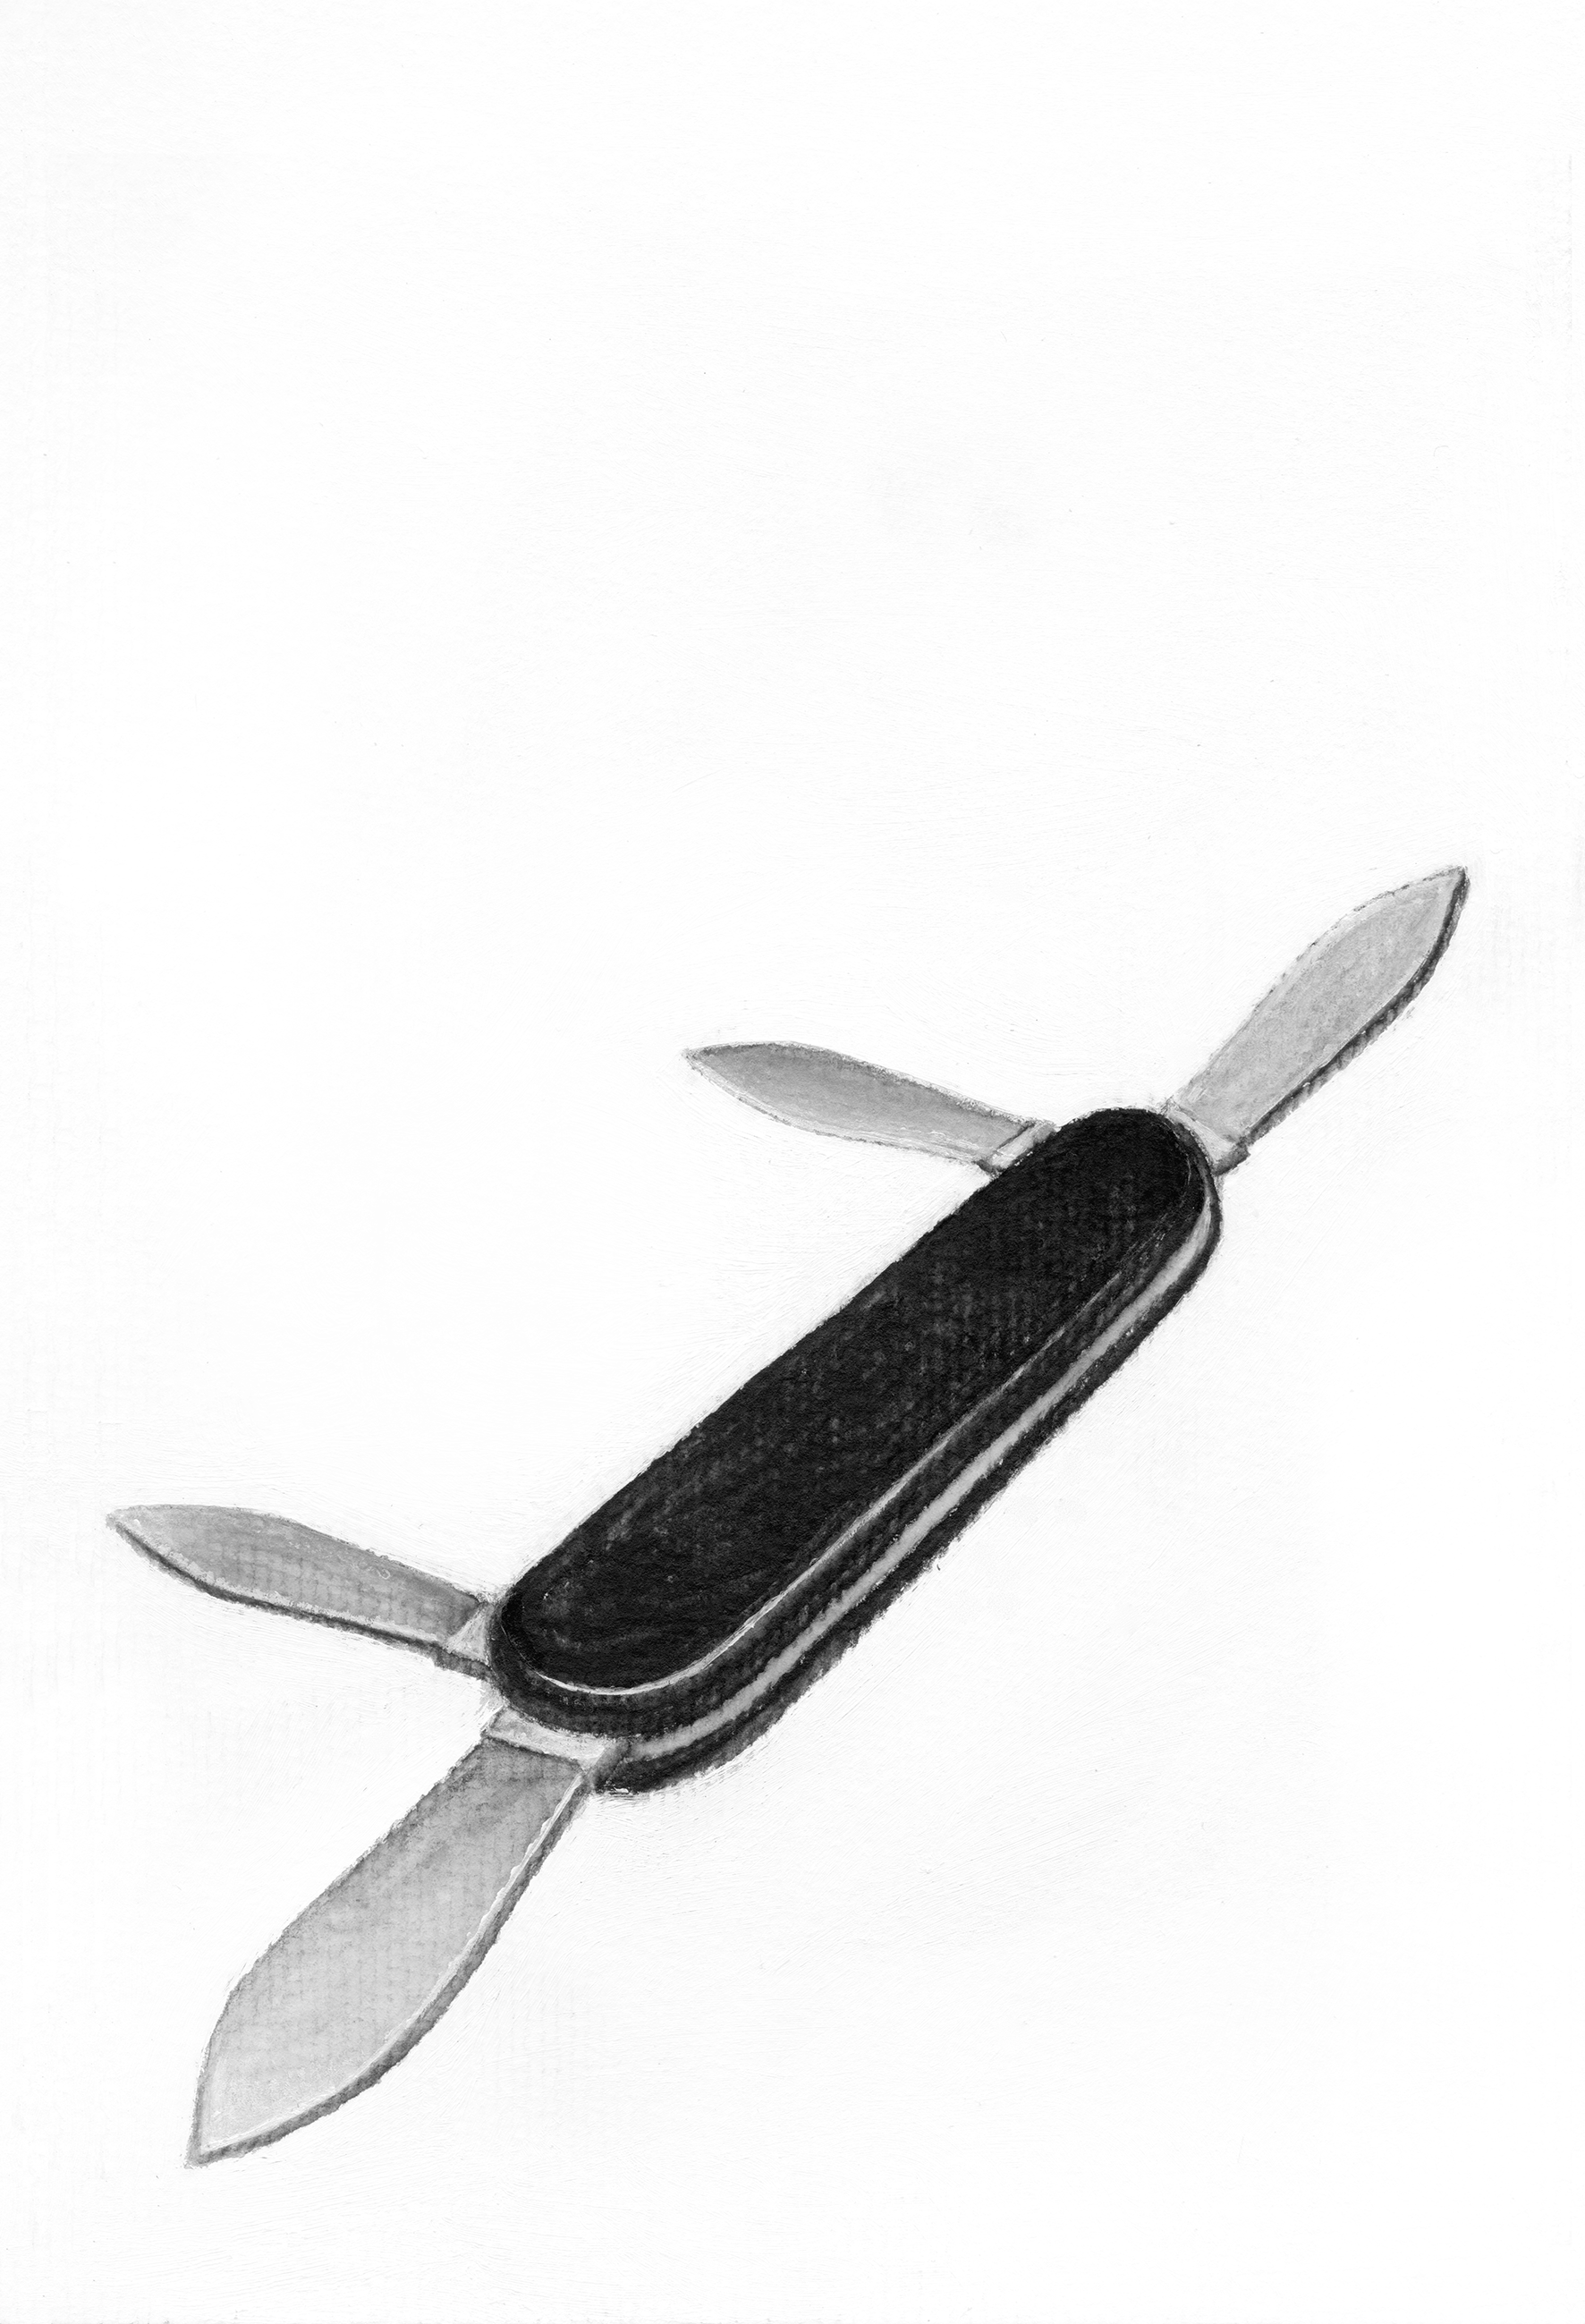
\includegraphics[width=155mm]{./imgs/2.pdf}
\end{figure}

\chapter{Como terminou uma noite tediosa}

À noite Nikita examinava as ilustrações da revista \emph{Niva}\footnote{\emph{Niva}
  (\emph{Seara})\emph{,} revista ilustrada de São Petersburgo cujos
  suplementos literários eram muito populares na época. Foi editada de
  1870 até 1918.} e lia suas explicações. Pouca coisa lá era
interessante.

Eis uma ilustração: uma mulher na entrada de uma casa com os braços nus
até o cotovelo; flores em seus cabelos dourados; sobre os ombros e aos
pés dela, viam"-se pombos. Do outro lado da cerca, um sujeito de rifle
nas costas com os dentes arreganhados.

O mais tedioso nessa ilustração era não ser possível compreender para
que ela fora desenhada. Na explicação estava escrito:

``Quem já não viu pombos domesticados, verdadeiros amigos do homem?
(Nikita pulou o que mais haviam escrito sobre os pombos.) Quem, de manhã, não
gosta de jogar grãozinhos a esses pássaros? Um talentoso pintor alemão,
Hans Wurst, retratou um desses momentos. A jovem Elza, filha de um
pastor, foi para a entrada de sua casa. Os pombos viram sua predileta e
alegremente se dirigiram aos pés dela. Vejam --- um pousou no ombro
dela, outros bicavam comida de sua mão. Um jovem vizinho, caçador,
admirava furtivamente a cena''.

Nikita imaginou que Elza alimentava os pombos, depois os alimentava de
novo e de novo, e não tinha nada mais para fazer além disso --- que
tédio. Seu pai, o pastor, também estava em algum lugar no recinto,
sentado numa cadeira, bocejando de tanto tédio. E o jovem vizinho, o que
arreganhou os dentes como se estivesse com dor de barriga, saía pela
estrada assim mesmo, com os dentes arreganhados, munido de um rifle que,
como era de se esperar, não atirava. O céu da imagem era cinzento, a luz
do sol era cinzenta.

Nikita lambeu a ponta do lápis e desenhou bigodes na filha do pastor.

A figura seguinte retratava a vista da cidade de Buzuluk:\footnote{Buzuluk,
  cidade ao sul da Rússia, hoje parte da província de Samara.} um poste
demarcador de distância, uma roda quebrada de carroça à margem da
estrada e, ao longe, casinhas de madeira, uma igrejinha e a chuva caindo
inclinada de uma nuvem.

Nikita bocejou, fechou a revista \emph{Niva} e, apoiando as costas na
cadeira, aguçou o ouvido. Do sótão vinham assobios e uivos prolongados.
Então se ouviu uma voz de baixo --- uuuuuuuuu ---, ela se arrastava,
enervava"-se, baforava. Depois, com um trinado, a voz ficava fina e
queixosa, assobiando por uma narina, martirizando"-se por ser fina como
um fiozinho. E voltava a descer para o baixo, baforando.

Sobre a mesa redonda estava acesa a lâmpada de um abajur branco de
porcelana. Alguém passou pesadamente pelo corredor do outro lado da
parede --- provavelmente o foguista --- e sob a lâmpada os cristais
tilintaram suavemente.

A mãezinha inclinou a cabeça sobre o livro, os cabelos dela eram
cinzentos, finos e se enrolavam na têmpora, onde havia uma marca de
nascença parecida com um grão de cevada. De tempos em tempos, cortava
as folhas com a agulha de tricô. O livro tinha capa cor de tijolo. O
armário do escritório do pai estava cheio de livros como aquele, todos
se chamavam \emph{Mensageiro da Europa}.\footnote{\emph{Mensageiro da
  Europa} (\emph{Viéstnik Evropy}), revista liberal político"-literária
  de Petersburgo publicada de 1866 a 1918.} É surpreendente como adultos
gostam de tudo o que é tedioso: ler um livro assim é como empilhar
tijolos.

Sobre os joelhos da mãe dormia um ouriço domesticado, Akhilka, com o
narizinho molhado de porco apoiado sobre as patinhas. Quando as pessoas
se recolhiam, ele, depois de dormir o dia todo, passava a noite andando
pelo quarto, batendo com as unhas, grunhindo, farejando em todos os
cantos, espiando nos buraquinhos dos ratos.

O foguista, atrás da parede, ressoou ao fechar a portinha de ferro, e
foi possível ouvir como ele remexia na estufa. O quarto cheirava a
reboco aquecido, a piso lavado. Era tedioso, mas aconchegante. E algo no
sótão tentava assobiar: ``iuu"-iuu"-iuu"-iuu"-iu''.

--- Mamãe, quem está assobiando? --- perguntou Nikita.

A mãezinha ergueu as sobrancelhas, sem parar de ler; já Arkádi
Ivánovitch, que pautava um caderno, de imediato, como se estivesse
esperando por essa oportunidade, falou sem titubear:

--- Quando nós falamos de algo inanimado, é necessário usar o pronome
``quê''.

``Buuuuuuuu'' --- ouviu"-se um uivo no sótão. A mãezinha levantou a
cabeça, prestou atenção, encolheu os ombros e cobriu"-os com o xale de
lã. O ouriço acordou e começou a fungar.

Então Nikita imaginou como, no sótão frio e escuro, a neve havia se acumulado
na claraboia. Entre as vigas gigantescas do teto, manchadas de sujeira
de pombos, encontravam"-se velhas cadeiras, poltronas e restos de sofás
com molas à mostra. Em uma dessas poltronas, ao lado da chaminé,
sentava"-se o ``Vento'': peludo, coberto de poeira e de teias de aranha.
Estava sentado calmamente e, apoiando as bochechas nas mãos, uivava:
``Que tédiooooo''. A noite longa, o sótão frio, e ele lá completamente
sozinho, uivando.

Nikita levantou"-se da cadeira e sentou perto da mãe. Ela, sorrindo\,carinhosamente,\,puxou"-o\,e\,o\,beijou\,na\,cabeça.

--- Não está na hora de você dormir, menino?

--- Não, mais meia hora, por favor.

Nikita encostou a cabeça no ombro da mãe. No fundo do quarto a porta
rangeu e apareceu o gato Vaska,\footnote{Vaska é apelido de Vassíli.}
de rabo para cima, com aparência dócil e bondosa. Abrindo a boca rosada,
ele miou, quase inaudível. Arkádi Ivánovitch perguntou, sem tirar os
olhos do caderno:

--- Vassíli Vassílievitch, veio a propósito de quê?

Vaska, aproximando"-se da mãezinha, fitou"-a com os olhos estreitos,
verdes e dissimulados, e miou mais alto. O ouriço voltou a fungar.
Nikita teve a impressão de que Vaska sabia de algo e veio contar.

O vento no sótão uivou desesperadamente. E, nesse momento, do lado de
fora, soaram um grito baixinho, um ranger de neve, um murmúrio de vozes.
A mãezinha se levantou rapidamente da cadeira. Akhilka, grunhindo, rolou
de seus joelhos.

Arkádi Ivánovitch correu até a janela e, olhando atentamente, exclamou:

--- Chegaram!

--- Meu Deus! --- disse a mãezinha, agitada. --- Será que é Anna
Apollóssovna?\ldots{} Nesta tempestade de neve\ldots{}

Minutos depois, Nikita, que estava no corredor, viu como a porta forrada
de feltro abriu"-se com dificuldade, trazendo uma lufada gelada, e
apareceu uma mulher alta e corpulenta, com duas peliças e um xale, toda
em neve. Ela segurava pela mão um menino de sobretudo cinza com
botões brilhantes e um \emph{bachlyk}. Atrás dele, batendo as botas de
feltro cobertas de gelo, entrou um cocheiro com barba de neve, pingentes amarelos
de gelo no lugar do bigode, e sobrancelhas peludas brancas. Em
seus braços, estava deitada uma menina vestida de uma peliça branca de
pele de cabra com o forro aparente. Com a cabeça reclinada no ombro do
cocheiro, ela estava com os olhos fechados e tinha um rostinho meigo e
astuto.

Ao entrar, a mulher alta exclamou, numa voz de timbre grave e forte:

--- Aleksandra Leóntievna, venha receber suas visitas --- e, levantando
as mãos, começou a desenrolar o xale. --- Não se aproxime, não se
aproxime, irá resfriar"-se. Mas essas suas estradas, devo dizer, são
terríveis\ldots{} Já perto de casa entramos em uns arbustos\ldots{}

Essa era a amiga da mãezinha, Anna Apollóssovna Bábkina, que sempre
morou em Samara. Seu filho, Víktor, esperando o momento de lhe tirarem o
\emph{bachlyk}, olhava para Nikita de rabo de olho. A mãezinha pegou do
cocheiro a menina adormecida, tirou"-lhe o chapéu de pele --- os cabelos
dourados se soltaram imediatamente --- e a beijou.

--- Lília, queridinha, chegaram.

A menina suspirou, abriu os grandes olhos azuis e suspirou mais uma vez,
despertando.

\chapter{Víktor e Lília}

Nikita e Víktor Bábkin acordaram de manhã bem cedo no quarto de Nikita
e, sentados em suas camas, franzindo o cenho, olhavam um para o outro.

--- Eu me lembro de você --- disse Nikita.

--- E eu também me lembro muito bem de você --- imediatamente respondeu
Víktor ---, uma vez você ficou na nossa casa, em Samara, e comeu tanto
pato com maçã que lhe deram óleo de rícino.

--- Bem, disso eu não me lembro.

--- Mas eu lembro.

Os meninos ficaram em silêncio. Víktor bocejou de propósito. Nikita
disse com desdém:

--- Eu tenho um preceptor, Arkádi Ivánovitch, terrivelmente severo, que
me sufoca com os estudos. Ele consegue ler qualquer livro em meia hora.

Víktor sorriu.

--- Eu estou no ginásio, no segundo ano. Nosso ginásio é tão severo que
me deixam constantemente sem almoço.

--- Isso não é nada --- disse Nikita.

--- Não é nada para você. Embora eu seja capaz de ficar mil dias sem
comer.

--- Ah é? --- disse Nikita. --- Você já experimentou?

--- Não, ainda não. Minha mãe não deixa.

Nikita bocejou e se espreguiçou:

--- Mas eu, sabe, anteontem derrotei Stiopka Karnaúchkin.

--- Quem é esse Stiopka Karnaúchkin?

--- O maioral da aldeia. Eu lhe acertei uma e ele caiu. Dei para ele um
canivete com quatro lâminas e ele me deu uma soqueira --- depois
mostrarei para você.

Nikita levantou"-se da cama e começou a se vestir, sem se apressar.

--- Olhe, eu consigo levantar o dicionário Makárov com uma mão --- disse
Víktor, com voz trêmula de despeito, mas era evidente que estava a ponto
de desistir.

Nikita aproximou"-se da estufa azulejada com leito, pulou nele sem
apoiar as mãos e de lá, dobrando a perna, saltou ao piso com um pé só.

--- Se mexer os pés rapidamente, a gente pode voar --- disse fixando os
olhos em Víktor.

--- Isso não é nada. Na nossa classe, muitos meninos voam.

Os dois se vestiram e foram para a sala de jantar, onde cheirava a pão
quente e a panquecas doces, e o samovar claro e bem polido exalava tanto
vapor que as janelas ficaram embaçadas.

Perto da janela estavam sentados a mãezinha, Arkádi Ivánovitch e a
menina da véspera, de nove anos, a irmã de Víktor, Lília. Do outro
quarto se ouvia o bramido grave de Anna Apollóssovna: ``Dê a toalha''.

Lília estava de vestido branco, com uma fita azul"-clara de seda amarrada
em um grande laço atrás. Em seus cabelos claros e ondulados havia outro
laço azul"-claro, em forma de borboleta.

Nikita, aproximando"-se dela, corou e fez uma reverência. Lília se virou
na cadeira, estendeu a mão e disse muito seriamente:

--- Bom dia, menino.

Quando ela disse isso, seu lábio superior se levantou.

Nikita tinha a impressão de que ela não era uma menina de verdade, por
ser assim tão bonitinha, especialmente os olhos --- azuis e mais
brilhantes do que a fita --- e os cílios --- que pareciam de seda. Assim
que Lília o cumprimentou, deixou de prestar atenção nele e pegou com as
duas mãos uma grande xícara de chá, abaixando o rosto. Os garotos
sentaram"-se à mesa lado a lado. Deu"-se que Víktor tomava chá como um
bebê --- curvando"-se sobre a xícara, sorvia o chá esticando os lábios
compridos para dentro dela. Às escondidas, colocava mais açúcar, até a
xícara ficar melada; então, com voz lânguida, pedia para diluir o chá
com água. Cutucando Nikita com o joelho, ele cochichou:

--- Você gosta da minha irmã, não é?

Nikita não respondeu e um rubor se espalhou pelo seu rosto.

--- Você deve tomar cuidado com ela --- sussurrou Víktor ---, a menina
se queixa de tudo para minha mãe.

Enquanto isso, Lília, terminando de tomar o chá, limpou a boca com o
guardanapo, desceu da cadeira sem pressa e, aproximando"-se de Aleksandra
Leóntievna, disse, educada e cuidadosamente:

--- Agradeço, tia Sacha.

Em seguida foi até a janela, subiu com os pés em uma enorme poltrona
marrom e, tirando do bolso uma caixinha com agulhas e linhas, começou a
costurar. Nikita agora via somente o grande laço em forma de borboleta,
duas madeixas pendentes e, entre elas, a pontinha exposta de sua
língua, que se movimentava --- ela ajudava Lília a costurar.

Nikita estava desconcertado. Ele quis mostrar a Víktor como saltar pelo
encosto da cadeira, mas Lília nem virou a cabeça, e a mãezinha disse:

--- Crianças, vão fazer barulho no quintal.

Os meninos se vestiram e saíram para o quintal. O dia estava brando e
enevoado. O sol avermelhado pairava baixo sobre nuvens compridas em
camadas, lembrando campos nevados. No jardim, as árvores estavam rosadas
e cobertas de geada. Sombras imprecisas na neve foram impregnadas pela
mesma luz quente. Fazia um silêncio fora do comum; apenas dois
cachorros, Charók e Katók, que estavam perto da entrada dos fundos,
rosnavam com as cabeças viradas uma para a outra. Ficaram muito tempo
rosnando, arreganhando os dentes e engasgando, até que um trabalhador de
passagem lhes jogou uma luva; então, tossindo de raiva, levantaram"-se
nas patas traseiras e brigaram tanto que pelo chegou a voar. Eles tinham
medo de outros cachorros, odiavam pedintes e, de noite, em vez de vigiar
a casa, dormiam debaixo da cocheira.

--- O que vamos fazer? --- perguntou Víktor.

Nikita olhou para um corvo desgrenhado e insatisfeito que voava da eira
ao curral. Não queria brincar e estava triste, sem saber por quê. Queria
sugerir que fossem à sala de estar e ficassem lá, sentados no sofá,
lendo alguma coisa, mas Víktor disse:

--- Ah, você só quer brincar com meninas.

--- Por quê? --- perguntou Nikita, enrubescendo.

--- Você sabe por quê.

--- Não me amole. Eu não sei de nada. Vamos até o poço.

Os garotos foram até o poço ao qual vacas, atravessando os portões, iam
beber água. Ao longe, Michka Koriachónok, estalando, como um estouro de
rifle, o chicote gigantesco de pastor, de repente gritou:

--- O Baian, o Baian, cuidado, Nikita!

Nikita olhou para trás. Separando"-se da manada, Baian, um touro comprido
cinza"-rosado, de testa larga com pelos encaracolados e chifres curtos,
foi na direção dos meninos.

``Mu"-u'' --- Baian mugia com voz entrecortada, batendo o rabo nos
flancos.

--- Víktor, corrа! --- gritou Nikita e, pegando"-o pela mão, correu na direção de
casa.

O touro, trotando, lançou"-se contra os meninos. ``Mu"-uuu!''

Víktor olhou para trás, gritou, caiu na neve e cobriu a cabeça com as
mãos. Baian já estava a cinco passos dele. Então Nikita se deteve e, instantaneamente
vermelho de raiva, correu até o touro, tirou o chapéu e
começou a bater na cara de Baian com ele:

--- Passe, passe!

O touro parou, abaixou os chifres. De um lado vinha correndo Michka
Koriachónok, estalando o chicote. Então Baian mugiu queixosamente,
deu"-lhe as costas e recuou para o poço. Nikita, de tão agitado, ficou com os
lábios trêmulos. Colocou o chapéu e se virou. Víktor já estava perto de
casa e de lá acenava com a mão. Nikita olhou sem querer para a janela
--- a terceira à esquerda da entrada principal. Viu dois olhos azuis
surpresos e sobre eles um laço azul"-claro em forma de borboleta. Lília,
subindo no peitoril da janela, olhou para Nikita e de repente sorriu.
Nikita imediatamente se virou. E não se voltou de novo para a janela.
Sentiu"-se alegre e gritou:

--- Víktor, vamos descer a montanha de trenó, rápido!

``Quando eu voltar para casa e passar pela janela, devo ou não devo
olhar para ela? Não, não vou olhar.''

\begin{figure}
\vspace*{-2.65cm}
\hspace*{-2.85cm}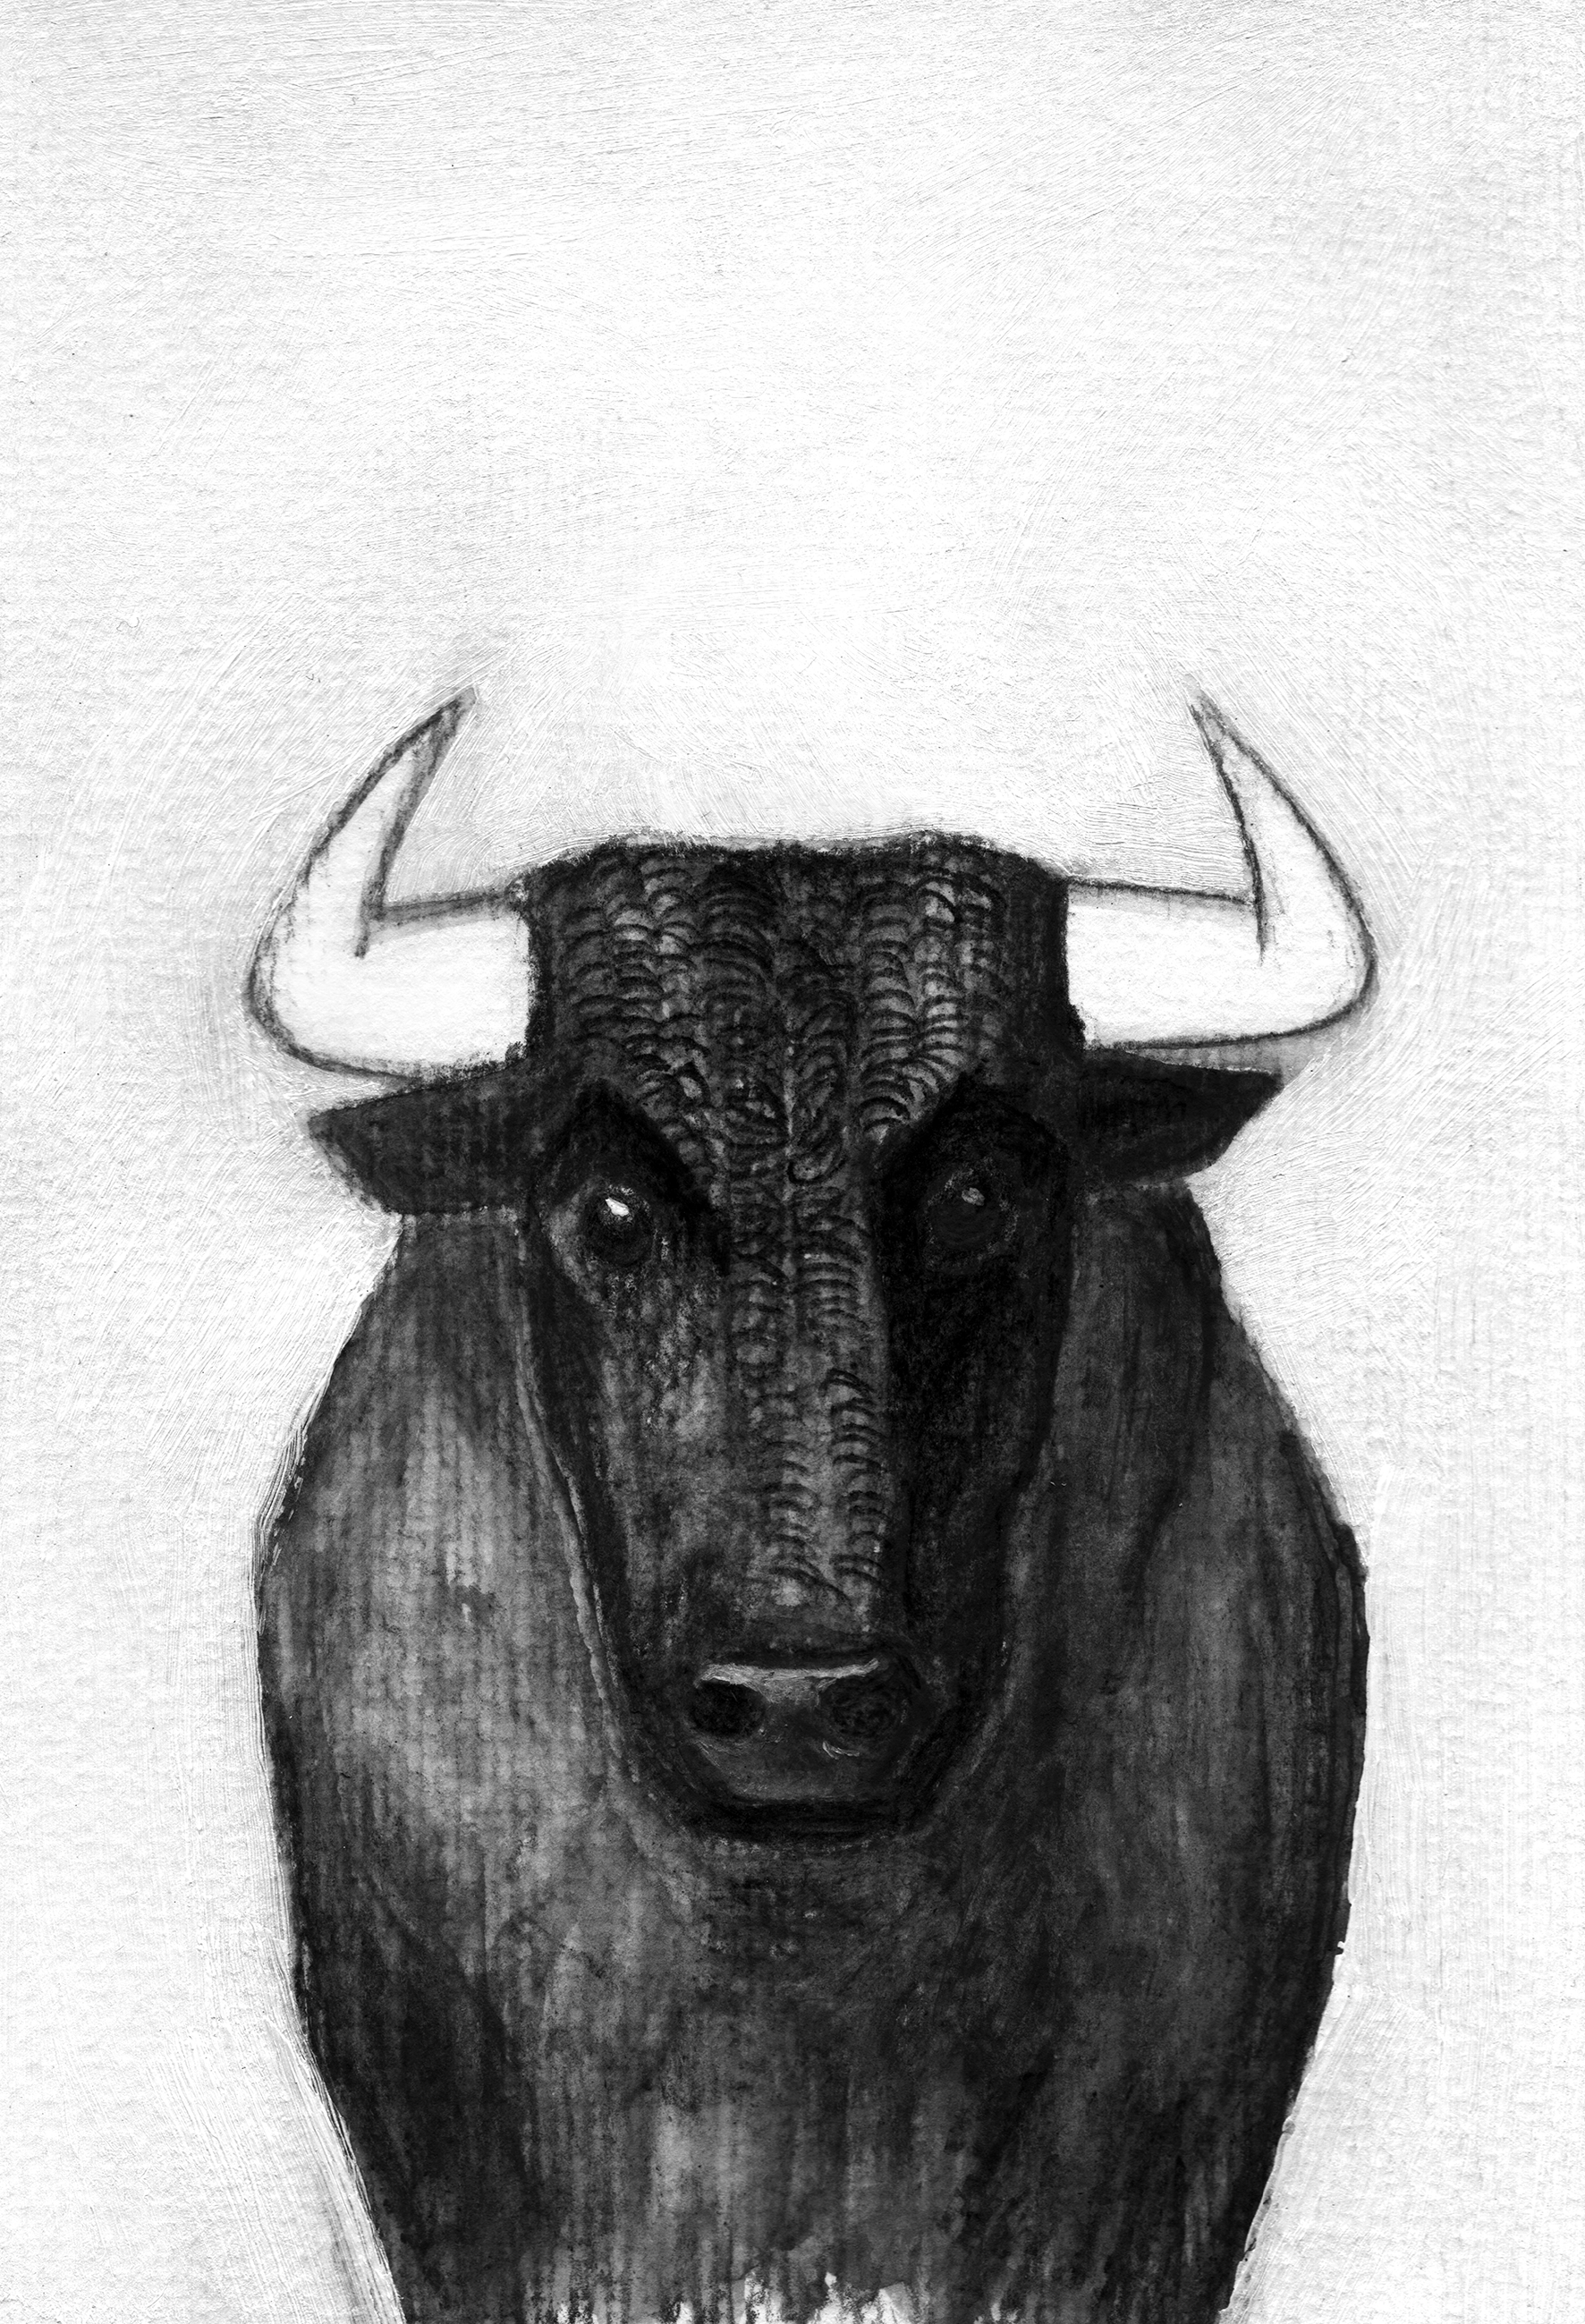
\includegraphics[width=155mm]{./imgs/8.pdf}
\end{figure}

\chapter{A caixinha da árvore de Natal}

Durante o almoço, Nikita tentava não olhar para Lília, mas, mesmo que
não tentasse, daria na mesma, porque entre ele e a menina estava sentada
Anna Apollóssovna, que, vestindo um colete de veludo vermelho e abanando
as mãos, falava com a voz tão alta e tão grossa que os pingentes de
vidro sob a lâmpada tilintavam.

--- Não e não, Aleksandra Leóntievna --- bramia ela ---, eduque seu
filho em casa. No ginásio há tantas desordens horrorosas que minha
vontade é pegar com as próprias mãos o diretor e o pôr porta afora\ldots{}
Víktor --- exclamou repentinamente ---, não é de sua conta o que sua mãe
está dizendo sobre adultos, você deve respeitar os superiores.
Aleksandra Leóntievna, veja nossos professores --- não passam de
parvalhões. Um mais tolo do que o outro. E o professor de geografia?
Qual é o sobrenome dele, Víktor?

--- Sinítchkin.

--- Mas eu digo que não é Sinítchkin, mas Siniávkin. Esse professor é
tão tolo que uma vez, na antessala, saindo de uma casa que havia
visitado, em vez do chapéu, pegou um gato que estava dormindo sobre um
baú e o colocou na cabeça\ldots{} Víktor, isso é modo de segurar o garfo e a
faca?\ldots{} Então, Aleksandra Leóntievna, o que mesmo eu queria lhe
dizer?\ldots{} Sim, eu trouxe uma mala cheia de todo tipo de quinquilharias
para a árvore de Natal\ldots{} Amanhã vamos pôr as crianças para fixar os
enfeites.

--- Mas eu acho --- disse a mãezinha --- que é necessário começar a
fixá"-los ainda hoje, senão não dará tempo de colar tudo.

--- Pois bem, faça como quiser. Eu vou escrever cartas. Obrigada pelo
almoço, minha amiga.

Anna Apollóssovna limpou os lábios com o guardanapo, afastou a cadeira
com estrondo e dirigiu"-se ao dormitório com a intenção de escrever
cartas, mas, um minuto depois, as molas da cama estalaram terrivelmente
no quarto, como se um elefante tivesse caído sobre elas.

Tiraram a toalha da grande mesa da sala de jantar. A mãezinha trouxe
quatro tesouras e começou a fazer cola. Fez assim: de um armarinho de
canto, onde ficava a farmacinha de casa, ela pegou um vidro de amido,
tirou uma colher de chá dele e verteu"-a num copo, onde despejou duas
colheres de água fria e começou a mexer a mistura até que virasse uma
pasta. Então verteu ali água fervente do samovar, continuando a mexer
intensamente, até que a pasta ficasse transparente como geleia --- e
finalmente conseguiu uma cola excelente.

Os meninos trouxeram a mala de couro de Anna Apollóssovna e colocaram"-na
sobre a mesa. A mãezinha abriu a mala e começou a tirar de lá folhas de
papel dourado liso com desenhos em relevo, folhas de papel prateado,
azul, verde e laranja, cartolinas, caixinhas com velas e castiçais para
árvore de Natal enfeitados com peixinhos e galos dourados, uma caixinha
com esferas ocas de vidro introduzidas em um pedaço de linha e outra
caixinha com esferas de alcinhas prateadas em cima e estampas pintadas
em cada quadrante de uma cor, depois uma caixa com petardos, maços de
fios dourados e prateados para bordado, lanterninhas com janelas
coloridas de mica e uma grande estrela. A cada nova caixinha as crianças
gritavam de alegria.

--- Lá ainda tem outras coisas boas --- disse a mãezinha, colocando as
mãos na mala ---, mas ainda não vamos desembrulhar tudo. Agora vamos
colar essas.

Víktor pôs"-se a colar as correntes de papel e Nikita os cones para
balas, enquanto a mãezinha cortava papel e papelão. Lília perguntou com
voz educada:

--- Tia Sacha, posso colar a caixinha?

--- Queridinha, pode colar o que quiser.

As crianças começaram a trabalhar em silêncio, respirando ruidosamente
pelo nariz, limpando as mãos sujas\,de cola na roupa. A mãezinha, nesse
meio"-tempo, contava que antigamente não existiam enfeites para árvore de
Natal e que tudo precisava ser feito com as próprias mãos. Por isso
havia pessoas capazes de criar para a árvore --- ela mesma chegara a ver
isso --- um verdadeiro castelo com torres, escadas espiraladas e pontes
levadiças. Diante do castelo ficava um lago feito de espelho cercado por
musgo. No lago flutuavam dois cisnes atrelados a um barquinho dourado.

Lília, ouvindo tudo, trabalhava calmamente e não dizia nada, apenas se
servia da língua nos momentos mais difíceis. Nikita deixou os cones de
papel e olhou para ela. A mãezinha havia saído. Víktor distribuía uns
dez \emph{archins} de correntes coloridas entre as cadeiras.

--- O que a senhorita está colando? --- perguntou Nikita.

Lília, sem levantar a cabeça, sorriu, recortou uma estrelinha de papel
dourado e a colou em uma tampa azul.

--- Para que precisa dessa caixinha? --- perguntou Nikita a meia voz.

--- Esta caixinha é para luvas de boneca --- respondeu Lília seriamente
---, como é menino, não vai entender --- então ergueu a cabeça e com
seus olhos azuis sérios encarou Nikita.

Ele começou a corar de maneira intensa e finalmente ficou roxo.

--- Como está vermelho --- disse Lília ---, parece uma beterraba.

E de novo se inclinou sobre a caixinha. Seu rosto tornou"-se astuto.
Nikita parecia grudado à cadeira. Não sabia o que dizer e não conseguia
sair do quarto de modo algum. A menina ria dele, mas ele não ficou
magoado nem zangado, e somente a admirava. De repente, Lília, sem
levantar os olhos, fez uma pergunta com outra voz, como se entre os dois
houvesse um segredo sobre o qual discutiam:

--- Gosta desta caixinha?

Nikita respondeu:

--- Sim, gosto.

--- Eu também gosto --- disse ela e meneou a cabeça, fazendo balançar
seu laço e suas madeixas. Queria acrescentar algo, mas, nesse momento,
Víktor se aproximou e, enfiando a cabeça entre Lília e Nikita, disse
rapidamente:

--- Que caixinha? Onde está, deixe ver?\ldots{} Que bobagem, é uma caixinha
comum. Como essa posso fazer quantas quiserem.

--- Víktor, palavra, eu vou dizer para mamãe que você não me deixa colar
--- queixou"-se Lília com voz trêmula. Ela pegou a cola e o papel e os
levou para o outro lado da mesa.

Víktor piscou para Nikita.

--- Eu disse que com ela tem que ter cuidado: é dedo"-duro.

Tarde da noite, Nikita, deitado na cama, no quarto escuro, cobrindo a
cabeça, perguntou debaixo do cobertor, com voz abafada:

--- Víktor, está dormindo?

--- Ainda não\ldots{} Não sei\ldots{} Que é?

--- Escute, Víktor\ldots{} Eu preciso contar um segredo terrível\ldots{} Víktor\ldots{}
Mas não durma\ldots{} Víktor, escute\ldots{}

--- A"-hã --- fiuiu --- respondeu Víktor.

\chapter{O que foi trazido na carroça separada}

Ainda de madrugada, durante o sono, Nikita ouviu alguém revolver as
estufas da casa e bater a porta no fim do corredor --- era o foguista
trazendo um feixe de lenha e tijolos de esterco e palha para o fogo.

Nikita acordou de felicidade. A manhã estava clara e gelada.

As janelas foram cobertas por uma camada densa de gelo dos galhos em
forma de garras. Víktor ainda estava dormindo. Nikita jogou"-lhe o
travesseiro, e o outro, resmungando, puxou o cobertor por cima da
cabeça. De felicidade, Nikita livrou"-se rapidamente do cobertor, se
vestiu e pensou --- aonde ir? E correu para o quarto de Arkádi
Ivánovitch.

Arkádi Ivánovitch acabara de acordar e, ainda deitado, lia aquela mesma
carta que já lera trinta vezes. Vendo Nikita, levantou os pés junto com
o cobertor, deixo"-os cair na cama e gritou:

--- Que acontecimento extraordinário! Levantou"-se antes de todos!

--- Arkádi Ivánovitch, que dia agradável.

--- O dia, irmãozinho, está formidável.

--- Arkádi Ivánovitch, queria perguntar uma coisa --- Nikita mexeu com o
dedo no batente ---, o senhor gosta dos Bábkin?

--- De qual Bábkin exatamente?

--- Das crianças.

--- Sim, sim\ldots{} E de qual criança exatamente você quer que eu goste?

Arkádi Ivánovitch disse isso com imensa rapidez, apesar do tom
corriqueiro. Apoiava a mão no travesseiro e dirigia o olhar a Nikita; é
verdade que não sorria, mas olhava"-o com bastante atenção. Ele também,
era evidente, sabia de alguma coisa. Nikita de repente se virou, saiu
correndo do quarto, pensou um pouco e foi ao quintal.

Uma fumaça azul elevava"-se em colunas sobre a ala dos criados, sobre a
casa de banhos na ravina e mais adiante, atrás do campo branco, sobre
toda a aldeia. Durante a noite, a geada baixou mais densa sobre as
árvores, e os enormes álamos negros da lagoa penderam completamente seus
galhos de neve, que podiam ser distinguidos com clareza no céu azul
gelado. A neve brilhava e estalava. O nariz pinicava e os cílios
grudavam.

Perto da entrada de serviço, ao lado de um monte de cinzas fumegantes,
Charók e Katók rosnavam um para o outro. Atolando na neve, Michka
Koriachónok, com um bastão na mão, atravessava o quintal, indo na
direção de Nikita --- pretendia fazer uns lançamentos de
\emph{kotiáchi}\footnote{\emph{Kotiáchi,} bolinhas feitas de uma mistura
  de esterco de vaca, palha e terra e então congeladas na neve.} no
gelo. Nesse ínterim, na estrada à direita da aldeia, apareceram carroças
de carga. Uma atrás da outra, subiam lentamente a ravina e se arrastavam
sobre a neve, baixinhas e escuras, ao longo da lagoa de baixo, rumo ao
dique.

Michka Koriachónok, encostando o dedão da luva no nariz, assoou"-se e
disse:

--- Nosso comboio está vindo da cidade, trouxeram presentes.

As carroças agora andavam sobre o dique, sob a abóboda gigantesca dos
salgueiros nevados, e já se podia ouvir o estalo da neve, o ranger dos
patins dos trenós e a respiração dos cavalos.

O primeiro a entrar no quintal, à frente do comboio, como sempre
ocorria, foi o trabalhador"-chefe, Nikífor, conduzindo uma grande égua
ruiva, Viesta. Nikífor, um velho atarracado, andava a passos lentos, ao
lado do trenó, vestindo botas de feltro cobertas de gelo enroladas com
uma corda. Seu casaco estava aberto, a gola de pele de carneiro
levantada, e o chapéu, a barba e as sobrancelhas cheios de neve. Viesta,
suja de suor, ofegava inflando os flancos e tinha vapor no hálito. Ao
andar, Nikífor se virou e, com a voz rouca e forte, gritou para as
carroças de trás:

--- Ei, virem para os celeiros. Escutem! A última carroça, siga para
casa.

Ao todo, no comboio havia dezesseis trenós. Os cavalos andavam
animadamente, exalando um cheiro forte de suor, os patins dos trenós
rangiam, os chicotes estalavam, vapor erguia"-se sobre o comboio.

Quando a última carroça deixou o dique e se aproximou, Nikita não
entendeu de imediato o que havia nela. Era algo de formato estranho,
verde, com uma faixa vermelha comprida. O coração dele acelerou. Sobre
um trenó com um segundo trenozinho acoplado atrás, um barco para
dois remos de proa afiada rangia e balançava. Ao lado, havia dois remos
verdes e um mastro com topo de cobre.

\textls[-15]{Então era esse o presente prometido na carta misteriosa!}

\chapter{A árvore de Natal}

Levaram uma grande árvore de Natal congelada para a sala de estar.
Pakhom ficou muito tempo martelando e aparando a árvore com um machado
para arrumá"-la numa base em forma de cruz. Finalmente, a árvore foi
levantada e se revelou tão alta que a pontinha superior, de um verde
suave, dobrou"-se perto do teto.

Ela exalava frio, mas aos poucos os galhos grudados descongelaram,
endireitaram, afofaram, e o cheiro da folhagem de abeto espalhou"-se pela
casa. As crianças trouxeram para a sala de estar uma porção de correntes
de papel e de caixinhas com enfeites, colocaram as cadeiras ao redor da
árvore e começaram a enfeitá"-la. Mas logo se verificou que não havia
enfeites o suficiente. Foram obrigados a sentar de novo para colar cones
de papel, deixar as nozes douradas, amarrar cordões prateados nos bolos
de mel e nas maçãs da Crimeia. Entretidas com esse trabalho, ficaram
sentadas a noite toda, até que Lília, abaixando a cabeça e amassando o
laço no cotovelo, dormiu na mesa.

Chegou a véspera de Natal. Terminaram de enfeitar a árvore,
envolveram"-na em uma teia dourada, penduraram as correntes e colocaram
velas em prendedores coloridos. Quando tudo estava pronto, a mãezinha
disse:

--- Agora, crianças, vão embora e até a noite não podem bisbilhotar
aqui.

Nesse dia, almoçaram tarde e às pressas, e as crianças só comeram bolo
de maçã. A casa estava agitada. Os meninos vagavam pela casa e
importunavam todo mundo perguntando: quando a noite vai começar? Até
Arkádi Ivánovitch, vestindo uma sobrecasaca de abas longas e uma camisa
engomada que de tão dura ficava em pé, não sabia o que fazer --- andava
de janela em janela e assobiava. Lília foi ficar com sua mãe.

O sol se arrastava até a terra com terrível lentidão, ficava rosado e
cobria"-se de nuvens escuras, e a sombra lilás do poço sobre a neve se
alongava. Finalmente, a mãezinha mandou que fossem se vestir. Nikita
achou sobre a cama uma camisa de seda azul, com bordados de abeto na
gola, na barra e nas mangas, um cinto torcido com borlas e bombachas de
veludo. Ele se vestiu e correu até a mãezinha. Ela alisou"-lhe o cabelo
com um pente, fazendo uma risca, pegou"-o pelos ombros, fitou"-o
atentamente no rosto e levou"-o até uma grande penteadeira de madeira
vermelha.

No espelho, Nikita viu um menino bem vestido e educado. Será que era
ele mesmo?

--- Ah, Nikita, Nikita --- disse a mãezinha, beijando"-o na cabeça ---,
se você fosse sempre assim.

Nikita saiu na ponta dos pés para o corredor e viu uma menina imponente,
de branco, vindo ao seu encontro. Ela estava com um lindo vestido de
sainhas de musselina e um grande laço branco no cabelo, e seis madeixas
caíam"-lhe sobre os ombros magrinhos, ladeando seu rosto, agora
irreconhecível. Aproximando"-se, Lília olhou com uma careta para Nikita.

--- Você achou que eu era um fantasma? --- perguntou ela. --- Com que se
assustou? --- e passou para o escritório, sentando"-se com os pés no
sofá.

Nikita foi atrás dela e também se sentou no sofá, na outra ponta. No
quarto, o fogo da estufa estava aceso, lenhas estalavam, desfazendo"-se
em carvões. Uma luz avermelhada iluminou as costas das poltronas de
couro, um canto de uma moldura dourada na parede e o busto de Púchkin\footnote{Aleksándr Púchkin (1799--1837), poeta e prosador que deu início à moderna literatura russa. Figura emblemática no país, morrera num duelo com o francês Georges Charles d’Anthès (1812--1895), depois de este haver cortejado Natália Gontcharova (1812--1863), esposa do escritor.}
entre os armários.

Lília estava sentada, imóvel. Era encantador quando a claridade do fogo
iluminava suas bochechas e seu narizinho empinado. Víktor apareceu de
uniforme azul com botões brilhantes e gola com galão, tão apertada que
era difícil até conversar.

Ele sentou"-se na poltrona e ficou em silêncio. Ao lado, na sala de
estar, ouviam a mãezinha e Anna Apollóssovna desembrulharem pacotes,
colocando algo no chão, e conversarem a meia voz. Víktor queria espiar
pelo buraco da fechadura, mas, do outro lado, o buraco estava tapado por
um papel.

Depois, no corredor, a porta bateu no batente e ouviram"-se vozes e
repetidos passos miúdos. Eram as crianças que tinham vindo da aldeia.
Nikita precisava correr para recebê"-las, mas não conseguia se mexer. Uma
luz azulada iluminou as ramagens de gelo da janela. Lília disse numa voz
fininha:

--- Uma estrela subiu.

Nesse momento as portas do escritório se abriram. As crianças saltaram
do sofá. Na sala de estar, a árvore de Natal resplandecia do chão até o
teto, com velas e mais velas. Parecia uma árvore de fogo, reluzia como
ouro, como faíscas e raios compridos. Emanava uma luz densa e quente com
cheiro de abeto, de tangerinas e de bolos de mel.

As crianças estavam paralisadas, atônitas. Abriram"-se as portas externas
para a sala de estar e, apertando"-se contra as paredes, entraram as
meninas e os meninos da aldeia. Todos tinham tirado as botas de feltro e
vestiam meias de lã, camisas vermelhas, cor"-de"-rosa, amarelas, lenços
amarelos, vermelhos e brancos.

A mãezinha começou a tocar uma polca no piano. Ao tocar, virava para a
árvore de Natal o rosto sorridente e cantava:


\begin{quotation}
Cegonhas de pernas largas

Não achavam a estrada\ldots{}
\end{quotation}

Nikita estendeu a mão para Lília. Ela lhe deu a sua, sem desviar os
olhos azuis das velas, e em cada olho dela se refletia uma árvore. As
crianças estavam imóveis. Arkádi Ivánovitch foi até o grupo de meninos e
meninas, pegou"-os pelas mãos e correu a galope com eles ao redor do
abeto. As abas de sua sobrecasaca tremulavam. Na corrida, pegou mais
dois, depois Nikita, Lília e Víktor, e finalmente toda a criançada
contornava numa dança de roda a árvore de Natal.

\begin{quotation}
O ouro eu vou esconder, esconder,

A prata eu vou esconder, esconder\ldots{}
\end{quotation}

\noindent{}--- cantavam as crianças da aldeia.

Nikita arrancou um petardo da árvore e rasgou sua embalagem: nele
havia um chapéu"-cone com uma estrela. Na hora estampidos se ouviram,
cheiro de pólvora se espalhou, e os cones de papel"-arroz começaram a
farfalhar.

A Lília coube um avental de papel com bolsinhos. Ela o vestiu. Suas
bochechas ficaram vermelhas como maçãs, os lábios estavam sujos de
chocolate. Ela ria o tempo todo, espiando uma enorme boneca colocada embaixo da árvore sobre um cesto com um enxoval de boneca.

Lá também, embaixo da árvore, estavam os pacotes de presentes, embalados em lenços coloridos, para as crianças da aldeia.
Víktor ganhou um regimento de soldados, com canhões e tendas. Nikita uma
verdadeira sela de couro, com rédeas e chicote.

Agora se podia ouvir como quebravam as nozes, estalando as cascas sob os
pés, e como as crianças, ofegantes, desembrulhavam os presentes.

Novamente a mãezinha se pôs a tocar e em volta da árvore
formaram uma roda, cantando, mas as velas já estavam se extinguindo e
Arkádi Ivánovitch, dando saltinhos, apagava"-as. A árvore de Natal
escureceu. A mãezinha fechou o piano e pediu que todos fossem tomar chá
na sala de jantar.

Mas nem assim Arkádi Ivánovitch sossegou --- formou uma corrente humana,
com ele à frente e vinte e cinco criancinhas atrás, correndo pelo
corredor até a sala de jantar.

Na antessala, Lília se separou da corrente e parou para recuperar o
fôlego, fitando Nikita com os olhos risonhos. Eles estavam perto dos
cabideiros com peliças penduradas. Lília perguntou:

--- Por que você está rindo?

--- É você que está rindo --- respondeu Nikita.

--- Por que você está olhando para mim?

Nikita enrubesceu, mas chegou mais perto de Lília e, sem que ele mesmo
compreendesse como tudo aconteceu, inclinou"-se na direção dela e a
beijou. Ela de pronto respondeu, numa fala apressada:

--- Você é um bom menino, eu não disse isso antes porque não era para
ninguém saber, é um segredo --- virou"-se e correu para a sala de jantar.

Depois do chá, Arkádi Ivánovitch organizou um jogo das
prendas,\footnote{No jogo das prendas (\emph{igrá v fánty}), cada
  participante, numa variação da brincadeira, deve colocar um objeto
  pessoal (um relógio, um lenço, uma pulseira, etc.) em uma sacola ou um
  chapéu. Um dos objetos é sorteado e um desafio é proposto ao seu dono
  para que ele possa recuperar sua prenda.} mas as crianças cansaram,
comeram muito e não entenderam bem o que era necessário fazer. Por fim,
um menininho de camisa de bolinhas adormeceu, caiu da cadeira e começou
a chorar sonoramente.

A mãezinha anunciou que a festa da árvore de Natal tinha acabado. As
crianças foram para o corredor, ao longo do qual estavam as botas de
feltros e os casaquinhos de pele. A turma toda se vestiu e foi junta
para o frio congelante.

Nikita acompanhou as crianças até o dique. Quando ele voltava sozinho
para casa, no alto do céu a lua reluzia num círculo pálido e matizado.
As árvores no dique e no jardim eram enormes e brancas e parecia terem
crescido sob a luz da lua. À direita um deserto branco se dirigia para
uma escuridão insondável de gelo. Ao lado de Nikita caminhava uma sombra
comprida com a cabeça grande.

Nikita tinha a impressão de caminhar dormindo por um reino encantado.
Somente em um reino encantado acontece algo tão estranho e ao mesmo
tempo tão alegre.

\chapter{A infelicidade de Víktor}

Nos últimos dias, Víktor fez amizade com Michka Koriachónok e ia com ele
até a lagoa de baixo para pôr fogo nos ``gatos''. Um dia queimaram um
``gato'' de tal jeito que o fogo que saiu do gelo ultrapassou a altura
de um homem. Depois, numa vala atrás do dique, construíram uma fortaleza
--- uma torre de gelo com um muro ao redor, ameias e portão. Então
Víktor escreveu uma carta aos meninos do outro lado:

``Vocês, do outro lado, ferreiros zarolhos que colocam ferraduras em
ratos, vamos dar uma surra em todos que nunca vão esquecer. Venham,
estamos esperando na fortaleza.

Víktor Bábkin, comandante e aluno do segundo ano''.

Esta carta foi pregada a uma vara que Michka Koriachónok levou para a
aldeia e cravou em um monte de neve, perto da isbá de Artamon. Siomka,
Lionka e o pequeno Artamon, Aliochka, Vanka Orelhas Pretas e Petruchka,
o sobrinho do camponês sem"-terra, subiram no monte de neve perto da vara
e ficaram muito tempo ameaçando os meninos do outro lado e atirando
bolinhas de esterco e palha em sua direção; depois foram até Michka
Koriachónok e tomaram lugar na fortaleza.

Víktor mandou que fizessem bolas e bolinhas de neve. Distribuíram tudo
ao longo dos muros da fortaleza, no interior, fixaram com um punhado de
juncos a vara na torre e ficaram à espera.

Nikita veio, examinou a fortificação e colocou as mãos nos bolsos:

--- Ninguém virá, a fortaleza não serve para nada; eu não quero brincar
com vocês, vou para casa.

--- O cavalheiro encontrou uma mocinha --- gritou Víktor do muro.

Os filhos de Artamon riram sonoramente. Vanka Orelhas Pretas assobiou
enfiando os dedos na boca. Nikita disse:

--- Se eu quisesse, derrubaria todos vocês, junto com essa fortaleza,
mas não quero sujar as mãos --- mostrou a língua para Víktor e foi para
casa cruzando a lagoa.

Algumas bolas de neve voaram atrás de Nikita, mas ele nem se virou. Os
que estavam na fortaleza não ficaram muito tempo esperando: por trás de
medas nevadas, vindos do outro lado da aldeia, apareceram os rivais.
Dirigiam"-se à fortaleza, com neve pelos joelhos. Eram uns quinze
meninos.

Fungando pelo nariz vermelho de frio, Víktor dizia que faria deles lenha
para queimar. Os olhos dele se agitavam. Os de lá aproximaram"-se e
assumiram posições diante do portão da fortaleza; alguns sentaram na
neve. Também vinha se arrastando com eles o menininho com o lenço da
mãe. Eram conduzidos por Stiopka Karnaúchkin. Examinando a
fortaleza, ele chegou pertinho do muro e disse:

--- Entreguem o garoto de botões brilhantes, nós vamos esfregar as
orelhas dele com neve\ldots{}

Víktor fungou, preocupado. Michka sussurrou: ``Jogue um belo torrão
nele, jogue!''. Víktor pegou uma bola de neve, arremessou"-a e errou o
alvo. Karnaúchkin recuou e ficou perto dos seus. Os garotos do outro
lado saltaram e começaram a fazer bolas de neve. Da fortaleza voaram
torrões na direção deles. Os filhos de Artamon atiravam com destreza.
Eles logo derrubaram o menininho com o lenço da mãe. Os de lá
retrucaram. Bolas de neve voavam de ambos os lados, como uma nuvem. A
vara com o emblema tombou na torre. Vanka Orelhas Pretas caiu do muro e
se entregou. De repente, derrubaram o boné de Víktor e, com outro
torrão, acertaram o rosto dele. Os garotos rivais uivaram, deram
gritos agudos, assobiaram e iniciaram o ataque\ldots{}

Abrindo uma brecha no muro, os defensores da fortaleza fugiram
correndo através do junco e pela lagoa congelada.

\chapter{O que havia no vasinho\break sobre o relógio de parede}

O próprio Nikita não entendia por que sentia tanto tédio ao brincar com
os garotos. Ele voltou para casa, tirou o casaco e, passando pelos
quartos, ouviu Lília dizendo:

--- Mamãe, pode me dar um pano limpinho, por favor? Minha boneca nova,
Valentina, está com dor na perna; estou preocupada com a saúde dela.

Nikita se deteve e de novo, como em todos aqueles dias, sentiu"-se
feliz. Uma felicidade tão grande que parecia que dentro dele havia uma
caixinha de música girando e tocando algo terno e alegre.

Nikita foi ao escritório, sentou"-se no sofá --- naquele mesmo lugar onde,
na antevéspera, Lília se sentara --- e dirigiu os olhos semicerrados
para as janelas desenhadas pelo frio. As ramagens tenras e
esmeradas pareciam de um reino encantado, do lugar onde a caixinha
mágica tocava, inaudível. Eram desenhos de galhos, folhas, árvores, de
estranhas figuras de animais e pessoas. Olhando para eles, Nikita teve a
impressão de que as palavras se juntavam sozinhas, cantando, e por isso,
por causa dessas palavras e desses cantos inquietantes, sentiu uma
coceirinha no cocuruto.

Ele desceu cuidadosamente da cadeira, achou na mesa do pai um quarto de
folha de papel e começou a escrever um verso com letras grandes:

\begin{quotation}
Ah, tu, bosque, meu bosque,

Meu encantado bosque,

Cheio de aves e animais

E feras joviais\ldots{}

Eu te amo, meu bosque\ldots{}

Como te amo, bosque\ldots{}
\end{quotation}

De repente continuar a escrever sobre bosques tornou"-se difícil. Nikita
roía a caneta, olhava para o teto. As palavras que escreveu também não
eram as que agora mesmo cantavam sozinhas, que pediam para serem livres.

Nikita releu os versos e continuou gostando deles. Dobrou o papelzinho
oito vezes, colocou"-o no bolso e foi à sala de jantar, onde Lília estava
costurando sentada perto da janela. A mão que segurava o papel no bolso
ficou suada, e ele hesitou em mostrar os versinhos.

Víktor chegou em casa ao entardecer, azul de frio e com o nariz inchado.
Anna Apollóssovna bateu palmas, irritada:

--- Quebraram o nariz dele de novo! Com quem você brigou? Responda já.

--- Não briguei com ninguém, o nariz inchou sozinho --- respondeu
sombriamente Víktor; em seguida, foi para seu quarto e deitou"-se na
cama.

Nikita foi atrás dele e se postou na frente da estufa. No céu
esverdeado, iam surgindo, como picadas de agulhas, estrelinhas. Nikita
disse:

--- Vou ler um versinho sobre o bosque, quer?

Víktor deu de ombros, apoiou os pés no encosto da cama e disse:

--- É bom você dizer a esse Stiopka Karnaúchkin que não apareça na minha
frente.

--- Sabe --- disse Nikita ---, esses versos descrevem certo bosque. É o
tipo de bosque que não se pode ver, mas que todo mundo conhece\ldots{} Se
você estiver triste, basta ler sobre esse bosque e tudo passa. Ou é
como, às vezes, quando você vê algo num sonho que é terrivelmente bom,
você não sabe o que é, mas é bom --- então você acorda e não consegue se
lembrar do que é\ldots{} Entende?

--- Não, não entendo --- respondeu Víktor ---, e não quero ouvir seus
versos.

Nikita suspirou, deteve"-se um momento em frente da estufa do quarto e
saiu. A grande antessala era iluminada pela estufa acesa, Lília estava
diante dela sentada sobre um baú coberto de pele de lobo e olhava o fogo
dançando.

Nikita se sentou no baú ao lado dela. A antessala emanava o calor do
fogo, o cheiro dos casacos que lá estavam pendurados e um aroma triste e
adocicado das tralhas abandonadas nas gavetas de uma enorme cômoda.

--- Vamos conversar --- disse Lília, pensativa ---, conte alguma coisa
interessante.

--- Quer que eu conte um sonho que tive não faz muito tempo?

--- Sim, conte o sonho.

Nikita começou a contar o sonho que tivera com o gato, contou dos retratos
que ganhavam vida, de como ele voava e o que vira voando sob o teto.
Lília ouvia atentamente, mantendo nos joelhos sua boneca na qual aplicou uma compressa.

Quando a história terminou, Lília se virou para ele, com os olhos
abertos de medo e de curiosidade, e perguntou sussurrando:

--- O que tinha no vasinho?

--- Não sei.

--- Lá devia ter alguma coisa de interessante.

--- Mas era um sonho.

--- Ah, tanto faz, devia ter olhado. Você é um menino, não entende nada.
Diga, o tal vasinho existe de verdade?

--- O relógio existe de verdade, mas do vasinho eu não me lembro. O
relógio está no escritório do meu avô, quebrado.

--- Vamos lá ver.

--- Lá está escuro.

--- Podemos pegar uma lanterninha da árvore de Natal. Vá, traga uma de
lá, por favor.

Nikita correu para a sala de estar, tirou da árvore uma lanterninha com
janelas coloridas de mica, acendeu"-a e voltou para a antessala.

Lília jogou sobre os ombros um grande xale de lã. As crianças foram em
surdina até o corredor e passaram rapidamente para a parte da casa
ocupada no verão. Em uma sala alta e escura, uma geada densa cobrira as
janelas e nelas a lua lançava sombras de galhos. Estava fresco,
cheirava a maçãs podres. As duas folhas da porta que dava para o quarto
escuro ao lado estavam entreabertas.

--- O relógio está aí? --- perguntou Lília.

--- Mais para a frente, no terceiro quarto.

--- Nikita, você não tem medo de nada?

Ele puxou uma porta, que rangeu queixosamente, e o ruído ressoou nos
quartos vazios. Lília agarrou a mão de Nikita. A lanterninha tremulou e
raios vermelhos e azuis correram pelas paredes.

As crianças entraram no quarto vizinho na ponta dos pés. A lua que
atravessava as janelas caía sobre o assoalho de quadrados azul"-claros.
Poltronas listradas estavam encostadas na parede, no canto ficava um sofá de
pés tortos. A cabeça de Nikita girava: já tinha visto aquele quarto,
exatamente como via agora.

--- Eles estão olhando para nós --- sussurrou Lília, apontando para os
dois quadros escuros pendurados na parede, o velhinho e a velhinha.

As crianças cruzaram o quarto correndo e abriram uma segunda porta. O
escritório estava inundado pela luz da lua. As portinhas de vidro das
estantes e o ouro das encadernações brilhavam. Sobre a lareira, a dama
com roupa de montaria, toda iluminada, fitava os que entraram, sorrindo
misteriosamente.

--- Quem é? --- perguntou Lília, encostando"-se em Nikita.

Ele respondeu sussurrando:

--- É ela.

Lília acenou positivamente com a cabeça e, de repente, olhando ao redor,
exclamou:

--- O vasinho, olhe, Nikita, o vasinho!

No fundo do escritório, em cima do antigo relógio de madeira vermelha
com um pêndulo imóvel, havia entre dois ornatos em caracol um vasinho de
bronze com a cara de um leão. Por algum motivo, Nikita nunca o havia
notado, mas agora o reconheceu: era o vasinho do seu sonho. Ele encostou
a cadeira no relógio, subiu nela, levantando"-se na ponta dos pés, enfiou o dedo
no vasinho e, apalpando"-o, sentiu poeira e algo duro.

--- Encontrei! --- exclamou apertando alguma coisa no punho e dando um
salto para o chão.

Nesse momento, algo bufou para ele debaixo do armário, olhos lilás
reluziram, e o gato Vassíli Vassílievitch, que estava caçando ratos na
biblioteca, saiu em disparada.

Lília agitou os braços e pôs"-se a correr e Nikita correu atrás dela,
muito assustado --- parecia que a mão de alguém tinha tocado o cabelo
dele. Ultrapassando as crianças, Vassíli Vassílievitch, de rabo baixo,
passou silenciosamente sobre os quadrados do assoalho iluminados pela
lua.

As crianças entraram correndo na antessala, sentaram no baú perto do
fogo, recuperando"-se do susto e retomando o fôlego. As bochechas de
Lília ardiam. Fitando Nikita diretamente nos olhos, ela disse:

--- Então?

Ele abriu os dedos. Na palma de sua mão havia um anel delicado com uma
pedrinha azul. Lília ficou sem palavras e ergueu os braços, surpresa.

--- Um anel!

--- Ele é mágico --- disse Nikita.

--- Escute, o que vamos fazer com ele?

Nikita, franzindo o cenho, pegou a mão dela e colocou o anelzinho no
dedo indicador. Lília disse:

--- Não, mas por que o deu para mim? --- ela olhou para a pedrinha,
sorriu, suspirou e, enlaçando Nikita pelo pescoço, beijou"-o.

Nikita enrubesceu tanto que foi obrigado a se afastar da estufa. Ainda
teve presença de espírito e disse:

--- Isso também é para a senhorita --- tirou do bolso o papelzinho
amassado, dobrado oito vezes, em que tinha escrito os versos sobre o
bosque, e o entregou à Lília.

Ela desdobrou"-o, começou a lê"-lo, movendo os lábios, depois disse,
pensativa:

--- Agradeço, Nikita, eu gosto muito dos seus versos.

\begin{figure}
\vspace*{-2.65cm}
\hspace*{-2.85cm}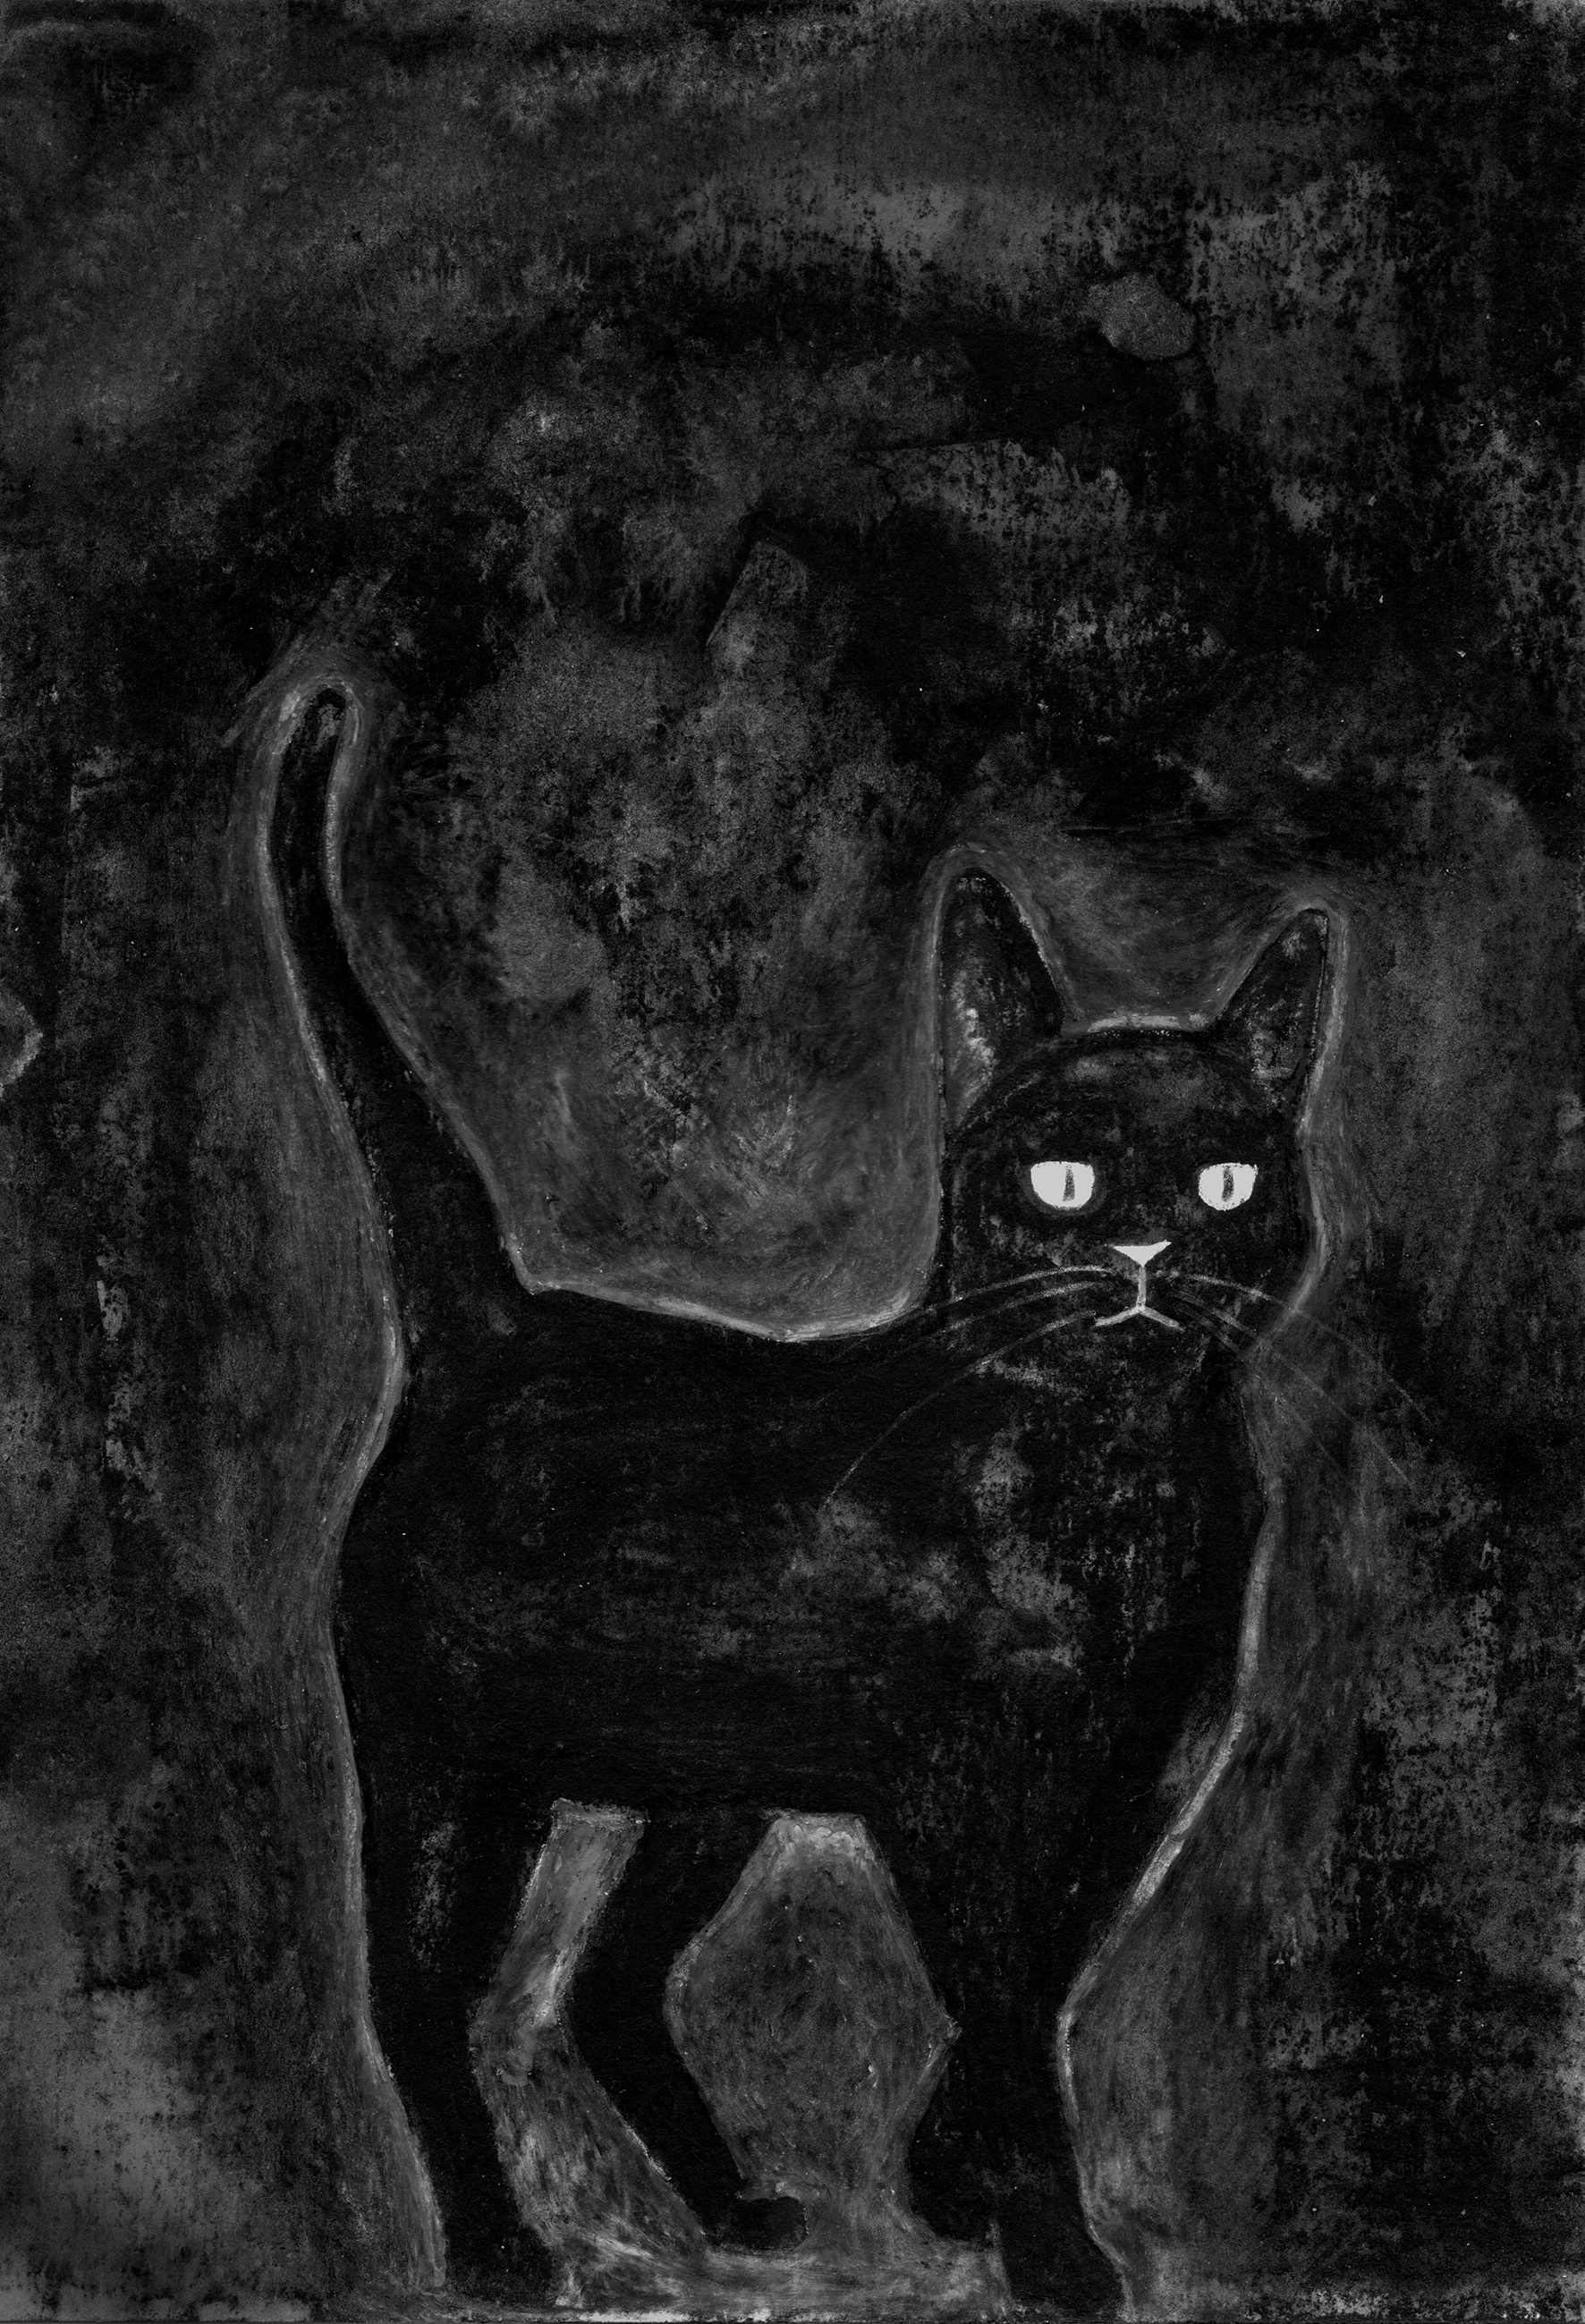
\includegraphics[width=155mm]{./imgs/6.pdf}
\end{figure}

\chapter{A última noite}

À noite, durante o chá, a mãezinha trocou alguns olhares com Anna
Apollóssovna e deu de ombros. Arkádi Ivánovitch, cujo rosto nada
expressava, estava sentado com a cabeça enfiada no copo, passando a
impressão de que, mesmo se o torturassem, ele não diria uma palavra.
Anna Apollóssovna, terminando a quinta xícara de chá com nata e
panquecas doces quentes, abriu um espaço na mesa bem à sua frente,
retirando todas as xícaras, pratinhos e migalhas, colocou sobre a toalha
a sua mão grande, com a palma voltada para baixo, e disse com voz
grossa:

--- Não, não e não, minha cara Aleksandra Leóntievna. Quando eu digo
algo, é definitivo; nada em exagero é bom. Escutem, crianças --- ela se
virou e tocou nas costas de Víktor com o dedo indicador, para que ele
não se curvasse ---, amanhã é segunda"-feira e vocês certamente se
esqueceram disso. Terminem de tomar o chá e vão dormir imediatamente. Ao
raiar do sol, nós partiremos.

Víktor silenciosamente projetou os lábios para a frente até que
passassem do nariz. Lília baixou os olhos rapidamente e se curvou sobre
a xícara. Os olhos de Nikita se nublaram e raios saíram do pavio da
lâmpada. Ele se virou e começou a olhar para Vassíli Vassílievitch.

O gato estava estirado no chão lavado, lambia a pata de trás esticada,
que nessa posição parecia uma pistola, e apertava os olhos. Não estava
entediado nem alegre, não precisava ter pressa para nada --- ``amanhã'',
pensava ele, ``vocês, humanos, terão um dia corriqueiro, voltarão a
resolver problemas de aritmética e a escrever ditados, mas eu, o gato,
que não celebrei as festas, não escrevi versos, não beijei a menina,
amanhã também estarei bem''.

Víktor e Lília terminaram de tomar o chá. Olhando para as sobrancelhas
grossas da mãe, que já começavam a menear, despediram"-se e saíram da
sala de jantar acompanhados por Nikita. Anna Apollóssovna gritou atrás
deles:

--- Víktor!

--- O que, mamãe?

--- Isso é jeito de andar?

--- O que tem?

--- Você anda como se estivesse sendo puxado por uma corda. Ande com
vontade. Não fique em zigue"-zague pelo quarto, aí está a porta.
Endireite as costas\ldots{}

As crianças saíram. Na antessala aquecida e a meia luz, onde deveriam
virar à direita, Nikita se deteve diante de Lília e, mordiscando os
lábios, disse:

--- A senhorita virá nos visitar no verão?

--- Isso depende da minha mãe --- respondeu Lília, com vozinha fina, sem
levantar os olhos.

--- Vai me escrever?

--- Sim, vou escrever cartas para você, Nikita.

--- Então, adeus.

--- Adeus, Nikita.

Lília acenou com o laço, estendeu a mão, as pontinhas dos dedos, e foi
para o seu quatro, sem se virar; ela caminhava bem aprumada, com passo
firme. Não era possível perceber nada apenas olhando para ela. ``Tem o
caráter muito reservado'', era o que Anna Apollóssovna dizia a seu
respeito.

Víktor, resmungando, colocava livros e brinquedos em um cesto, descolava
figuras e as guardava em uma caixinha e, arrastando"-se debaixo da mesa,
procurava seu canivete, ao passo que Nikita não disse uma palavra;
rapidamente tirou a roupa, cobriu"-se com o cobertor até a cabeça e
fingiu dormir.

Ele tinha a impressão de que o mundo havia acabado. Nos olhos tomados
pelo sono, surgiu pela última vez, como uma sombra na parede, um enorme
laço que ele agora lembrará pelo resto da vida. Ao dormir, ouvia vozes,
alguém se aproximava de sua cama, e as vozes se afastavam. Viu galhos
tépidos em forma de garras, grandes árvores, uma estrada avermelhada
atravessando com facilidade um matagal que se abria diante dela. Era
surpreendentemente agradável ficar nessa floresta estranha, matizada de
vermelho, e dava vontade de chorar de uma tristeza nunca sentida. De
repente, a cabeça de um selvagem de pele vermelha e óculos dourados
apareceu entre folhas de bardana: ``Ah, você ainda está dormindo!'',
gritou com voz troante.

Nikita abriu os olhos. Sobre seu rosto caía a luz quente da manhã.
Diante da cama estava Arkádi Ivánovitch, que, tocando repetidamente na
ponta do próprio nariz, dizia:

--- Levante, gaiato, levante.

\chapter{Separação}

Em janeiro, o pai de Nikita, Vassíli Nikítievitch, enviou uma carta.

``\ldots{} Já estou em desespero porque o processo da herança ainda está me
retendo, querida Sacha --- está claro que serei obrigado a ir até Moscou
para cuidar disso. Em todo caso, na quaresma estarei com vocês\ldots{}''

A mãezinha se entristeceu ao ler a carta e à noite mostrou"-a a Arkádi
Ivánovitch, dizendo:

--- Que essa herança vá com Deus se ela traz tantos desgostos; passamos
o inverno todo separados. Tenho até a impressão de que Nikita começou a
esquecer o pai.

Ela se virou e se pôs a olhar para a janela escura coberta de gelo. Do
lado de fora, a noite era erma e gelada, no jardim as árvores estalavam
tão fortemente que tudo estremecia em casa, as vigas do sótão trincavam
e, de manhã, veriam pardais mortos na neve. A mãezinha limpou levemente
os olhos com o lenço.

--- Sim, separação, separação --- disse Arkádi Ivánovitch, pensativo,
talvez se referindo à sua própria separação, e esticou a mão no bolso
atrás da carta.

Enquanto isso, Nikita desenhava o mapa da América do Sul --- tivera
nesse dia uma longa conversa com a mãezinha, que estava inquieta e
tentava mostrar que durante as festas ele ficara preguiçoso e
relaxado, e estava se preparando, pelo visto, para se tornar um escrivão
de povoado ou um telegrafista da estação Bezentchuk.\footnote{Bezentchuk,
  localidade pertencente ao distrito de Samara.} ``À noite, em vez de
figuras bobas'', disse ela, ``vai desenhar a América do Sul para mim.''

Nikita desenhava a América e se perguntava --- teria realmente se
esquecido do pai? Não. Em vez do rio Amazonas, lá, onde se cruzam a
latitude e a longitude, ele viu o rosto alegre do pai, de bochechas
vermelhas, olhos e dentes brilhantes, a barba escura dividida em duas
partes, a voz sonora e o riso solto. Era possível ouvi"-lo falar por
horas, morrendo de rir das histórias que contava. A mãezinha
frequentemente o repreendia por ser despreocupado e imprudente, mas isso
ocorria por ele ter um caráter muito vivo. Por exemplo, um dia lhe
passou pela cabeça a ideia de que as rãs, que abundavam nas três lagoas
da propriedade, morriam inutilmente; e por noites a fio ele falou sobre
como as rãs deviam ser alimentadas, cultivadas, tratadas e enviadas em
barris a Paris. ``Você está rindo'', dizia ele à mãezinha, que ria até
as lágrimas ouvindo essas histórias, ``mas me verá enriquecer com essas
rãs''. O pai mandou instalar gaiolas de pesca nas lagoas, cozinhou uma
mistura para alimentá"-las e trouxe rãs experimentais para casa, até que
a mãezinha anunciou: ``ou eu, ou as rãs'', disse que as temia com medo
mortal e que tinha nojo de morar numa casa cheia dessa imundície. Uma
vez, o pai viajou à cidade e enviou de lá, num comboio de carroças,
velhas portas e caixilhos de carvalho e uma carta: ``Querida Sacha,
consegui comprar a um preço vantajoso um lote de caixilhos e de portas.
Foi mais do que oportuno, já que você, como deve lembrar, sonhava em
construir um pavilhão na colina dos álamos. Eu já falei com um
arquiteto, que nos aconselha a construir um pavilhão de inverno, para
podermos morar nele também no frio. Já estou empolgado com a ideia, pois
a nossa casa fica num barranco, sem vista nas janelas''. A mãezinha caiu
no choro; o salário de Arkádi Ivánovitch não era pago já pelo terceiro
mês, e de repente novos gastos\ldots{} Recusou categoricamente a construção
do pavilhão, e os caixilhos e as portas ficaram para apodrecer num
galpão. Então o pai foi tomado por outra febre --- melhorias agrícolas
---, um novo fracasso: ele encomendou máquinas da América e as trouxe
pessoalmente da estação; zangava"-se ao ensinar os trabalhadores a
operá"-las, gritando para todos: ``Tomem cuidado, canalhas, tomem
cuidado!''.

Depois de um tempo, a mãezinha perguntou ao pai:

--- Então, como está sua incrível ceifadeira?

--- O que tem? --- o pai tamborilava no vidro da janela. --- Uma máquina
magnífica.

--- Eu a vi, está lá parada no galpão.

O pai deu de ombros e rapidamente alisou a barba dividida em duas
partes. A mãezinha perguntou docilmente:

--- Ela já quebrou?

--- Esses americanos idiotas --- disse o pai, fungando ---, inventam
máquinas que quebram a todo instante. Não tenho nada com isso.

Ao desenhar o rio Amazonas com seus afluentes, Nikita pensava no pai com
amor e ternura. Sua consciência estava tranquila --- fora à toa que a
mãezinha dissera que ele o havia esquecido.

De repente, a parede deu um estalo, como o de uma pistola. A mãezinha
deu um grito e deixou cair o tricô no chão. Debaixo da cômoda, o ouriço
Akhilka grunhiu e bufou de raiva. Nikita olhou para Arkádi Ivánovitch,
que fingia estar lendo, mas na realidade seus olhos estavam fechados,
embora não estivesse dormindo. Nikita tinha pena de Arkádi Ivánovitch:
pobrezinho, sempre pensando em sua noiva, Vassa Nílovna, uma professora
na cidade. É isso que separação quer dizer!

Nikita apoiou a bochecha na palma da mão e começou a pensar na sua
própria separação. Nesse canto da mesa costumava se sentar Lília, mas
ela não estava mais lá. Que tristeza --- ela estava, e agora não está.
Eis a manchinha na mesa onde ela derramara goma"-arábica. E nessa parede
a sombra do laço dela se refletia. ``Os dias felizes ficaram para
trás.'' Ele sentiu um comichão na garganta por causa dessas palavras
de tristeza incomum que tinha acabado de inventar. Para não esquecê"-las,
anotou"-as embaixo da América: ``Os dias felizes ficaram para trás'', e,
continuando a desenhar, conduziu o rio Amazonas para o lado errado,
passando pelo Paraguai e pelo Uruguai para desembocar na Ilha da Terra
do Fogo.

--- Aleksandra Leóntievna, acho que a senhora tem razão: esse menino
está se preparando para ser telegrafista da estação Bezentchuk --- com
uma voz calma de dar arrepio, falou Arkádi Ivánovitch, que já havia
algum tempo que observava o que Nikita fazia com o mapa.

\chapter{Dia a dia}

O frio ficou mais forte. Ventos cortantes cobriam as árvores de geada. A
neve se revestiu de uma crosta dura de gelo, e por ela lobos famintos e
com frio, sozinhos ou em dupla, aproximavam"-se de noite da propriedade.

Pressentindo cheiro de lobo, Charók e Katók começaram a ganir de
tristeza, a uivar baixinho, então meteram"-se embaixo da cocheira e
uivaram de lá, com vozes agudas e nauseantes: u"-u"-u"-u"-u\ldots{}

Os lobos atravessaram a lagoa e ficaram no meio do junco, farejando o
cheiro de uma casa habitável. Ao tomar coragem, passaram às escondidas
para o jardim, sentaram"-se na clareira nevada diante da casa, fitando
com olhos brilhantes as janelas escuras cobertas de gelo, ergueram as
fuças para a escuridão gelada e começaram a uivar, primeiro baixo, como
um resmungo, depois mais alto, num crescendo, ávidos, sem respirar, até
ficarem estridentes.

Por causa dos gritos dos lobos, Charók e Katók enfiaram a cara na palha e
se deitaram quase sem sentidos sob a cocheira. Na ala dos criados, o
carpinteiro Pakhom se virou no leito sobre a estufa, cobrindo"-se com uma
peliça de carneiro, e balbuciou, meio dormindo:

--- Oh, Senhor, como são pesados os nossos pecados.

Em casa os dias eram corriqueiros. Todos se levantavam muito cedo,
quando, do outro lado das janelas azul"-escuras, transpareciam no céu as
faixas rubras do amanhecer, e os vidros com uma penugem de neve aos
poucos começavam a clarear e a azular na parte de cima.

Em casa, ouviam"-se as portinhas das estufas baterem. Na cozinha, a
lâmpada de lata a querosene ainda estava acesa. Cheirava a samovar e a
pão quente. Não demoravam no café da manhã. A mãezinha logo limpava a
mesa de refeições e colocava a máquina de costura sobre ela. Aparecia a
costureira da casa, que tinha sido trazida da vila Pestravka, Sônia ---
manca e bexiguenta, com os dentes da frente gastos de tanto roer linhas
de costura ---, e costurava com a mãezinha roupas do dia a dia.
Durante o trabalho, conversavam em voz baixa e rasgavam chita fazendo
estalidos. A costureira Sônia era moça muito maçante --- parecia ter
ficado escondida atrás de um armário por anos, depois a encontraram,
limparam"-na um pouco e a colocaram para costurar.

Arkádi Ivánovitch, nesses dias, acelerou os estudos e deu --- como
gostava de se expressar --- um salto: começou a ensinar a álgebra, uma
matéria sem graça em alto grau.

Ao estudar aritmética, pelo menos era possível pensar em várias coisas
inúteis e curiosas: em tanques enferrujados com ratos mortos para onde a
água fluía em três canos; no eterno ``alguém'' vestindo sobrecasaca de
oleado, de nariz comprido, que misturava três tipos de cafés ou que
comprava tantos \emph{zolotniks}\footnote{\emph{Zolotnik}, medida russa de
  peso equivalente a 4,26 gramas.} de cobre; ou naquele lojista infeliz
com suas duas peças de tecido. Quanto à álgebra, não havia em que se
agarrar, não havia nada de vivo nela, pelo menos a brochura tinha cheiro
de cola de marceneiro e, quando Arkádi Ivánovitch explicava as regras,
inclinando"-se sobre a cadeira de Nikita, seu rosto redondo como uma
jarra refletia"-se no tinteiro.

Ao dar aulas de história, ficava de costas para a estufa. Contrastando
com o branco dos azulejos, sua sobrecasaca preta, a barba ruiva e os
óculos dourados sobressaíam lindamente. Contando como Pepino, o
Breve,\footnote{Pepino \textsc{iii}, o Breve ou o Moço (c.a. 714--768), filho
  mais novo de Carlos Martel, foi rei dos francos (751--768) e pai de
  Carlos Magno.} em Soissons, uma vez partira uma caneca com a mão,
Arkádi Ivánovitch, com um rápido movimento, cortou o ar com a mão.

--- Você deve entender --- dizia a Nikita --- que pessoas como Pepino, o
Breve se destacavam pela vontade inabalável e pelo caráter destemido.
Elas não se esquivavam do trabalho como alguns aqui, não ficavam a cada
instante olhando o tinteiro em que não há nada escrito, nem conheciam
palavras vergonhosas como ``não consigo'' e ``estou cansado''. Essas
pessoas nunca davam de enrolar o cabelo na testa, em vez de aprender a
álgebra. Por isso --- ele levantou o livro e colocou o dedo no meio dele
--- elas até hoje nos servem de exemplo.

Depois do almoço a mãezinha, como de costume, disse a Arkádi Ivánovitch:

--- Se hoje fizer menos vinte graus de novo, Nikita não vai passear.

Arkádi Ivánovitch, como de costume, aproximou"-se da janela e bafejou o
vidro na direção do termômetro fixado do lado de fora.

--- Vinte um e meio, Aleksandra Leóntievna.

--- Eu imaginei --- disse a mãezinha ---, Nikita, vá se ocupar com
alguma coisa.

Nikita, como de costume, foi ao escritório do pai, subiu no sofá de couro perto da estufa e abriu um livro mágico de Fenimore Cooper.

O escritório aquecido estava tão silencioso que nos ouvidos soava um
tinido quase inaudível. Que histórias extraordinárias podemos inventar
quando estamos sozinhos num sofá ao som desse tinido. Uma luz branca
jorrava dos vidros congelados. Nikita lia Cooper; depois, franzindo o
cenho por muito tempo, sem início nem fim, imaginava a si mesmo nas
pradarias amplas e verdejantes com ondas de capim, farfalhando ao vento;
mustangues malhados relinchando ao saltar e virando a cara alegre para
ele; os desfiladeiros escuros das Cordilheiras; uma queda d'água
prateada e sobre ela o chefe dos hurões, um indígena adornado de penas,
que tinha um rifle comprido e estava parado no alto de um penhasco que
lembrava um pão de açúcar. Numa floresta densa, entre as raízes de uma
árvore gigantesca, sentava"-se numa pedra ele próprio, Nikita, com a
bochecha apoiada no punho. A seus pés brilhava uma fogueira. Na floresta
estava tão silencioso que se ouvia um tinido nos ouvidos. Ele estava ali
à procura de Lília, que havia sido covardemente raptada. Realizava
várias façanhas, muitas vezes conduzia Lília no dorso de um mustangue
selvagem, subia pelos desfiladeiros, com um tiro certeiro derrubava do
pico do pão de açúcar o chefe dos hurões, que sempre reaparecia no mesmo
lugar; Nikita raptava e salvava Lília, e a raptava e a salvava de novo,
sem início nem fim.

Quando o frio e a mãezinha permitiam que colocasse o nariz para fora de
casa, Nikita saía para vaguear sozinho pelo quintal. As antigas brincadeiras
com Michka Koriachónok eram agora enfadonhas para ele, e ultimamente
Michka passou a ficar mais na ala dos criados entretendo"-se com o baralho --- ``o
jogo do nariz'' ou ``o jogo do sabichão'', em que o perdedor era puxado
pelo cabelo.

Uma vez Nikita se aproximou do poço e lembrou: vira dali, na janela de casa, um
laço azul"-claro que não existia igual no mundo. Agora a janela estava
vazia. Ali, perto da cocheira, Charók e Katók desenterraram da neve uma
gralha morta --- era a mesma gralha que Lília vira e, agachando"-se perto
dela, dissera: ``Que dó, Nikita, olhe, um passarinho morto''. Nikita
tirou o pássaro dos cachorros, levou"-o para trás da casinha da adega e
lá o enterrou.

Passando pelo dique, Nikita se lembrou de como, depois da festa de Natal, andara ali à noite ao longo de salgueiros enormes, translúcidos à luz da lua,
com sua própria sombra deslizando ao lado. Por que, naquela época,
valorizara tudo isso tão pouco? Devia ter fechado os olhos e sentido
como era feliz. Mas, agora, um vento lacerante zunia através dos
salgueiros escuros e congelados, na lagoa o morro de gelo pelo qual ele
e Lília tinham descido de trenó estava repleto de neve. Lília
semicerrava os olhos, em silêncio, agarrando"-se fortemente às laterais
do trenó. Todos os rastros tinham sido encobertos pela neve.

Nikita caminhou pela crosta de gelo ainda firme para além do quintal,
para onde o vento do Norte juntara montes de neve da altura dos telhados
de palha. Dali era possível ver o campo plano e branco --- um deserto
que se unia ao céu através da bruma gelada. Um vento rasteiro soprava
como fumaça. Levantava a barra de seu casaco de pele de carneiro. A neve
salpicava do topo de um monte. Ele próprio não sabia por que sentia
desejo de ficar olhando para aquele deserto.

A mãezinha começou a notar que Nikita estava triste e conversou a esse
respeito com Arkádi Ivánovitch. Decidiram parar com as aulas de álgebra,
mandar Nikita dormir mais cedo e ``rolar nele'', como Arkádi Ivánovitch
disse de forma não muito arguta, óleo de rícino.

Todas as medidas foram tomadas. Segundo observações de Arkádi
Ivánovitch, Nikita ficou mais alegre. Mas a verdadeira cura veio depois
de três semanas: um vento forte e úmido do Sul envolveu os campos, o
jardim e a propriedade em uma bruma cinzenta de nuvens vazadas que
corriam furiosas rente à terra.

\begin{figure}
\vspace*{-2.65cm}
\hspace*{-3.25cm}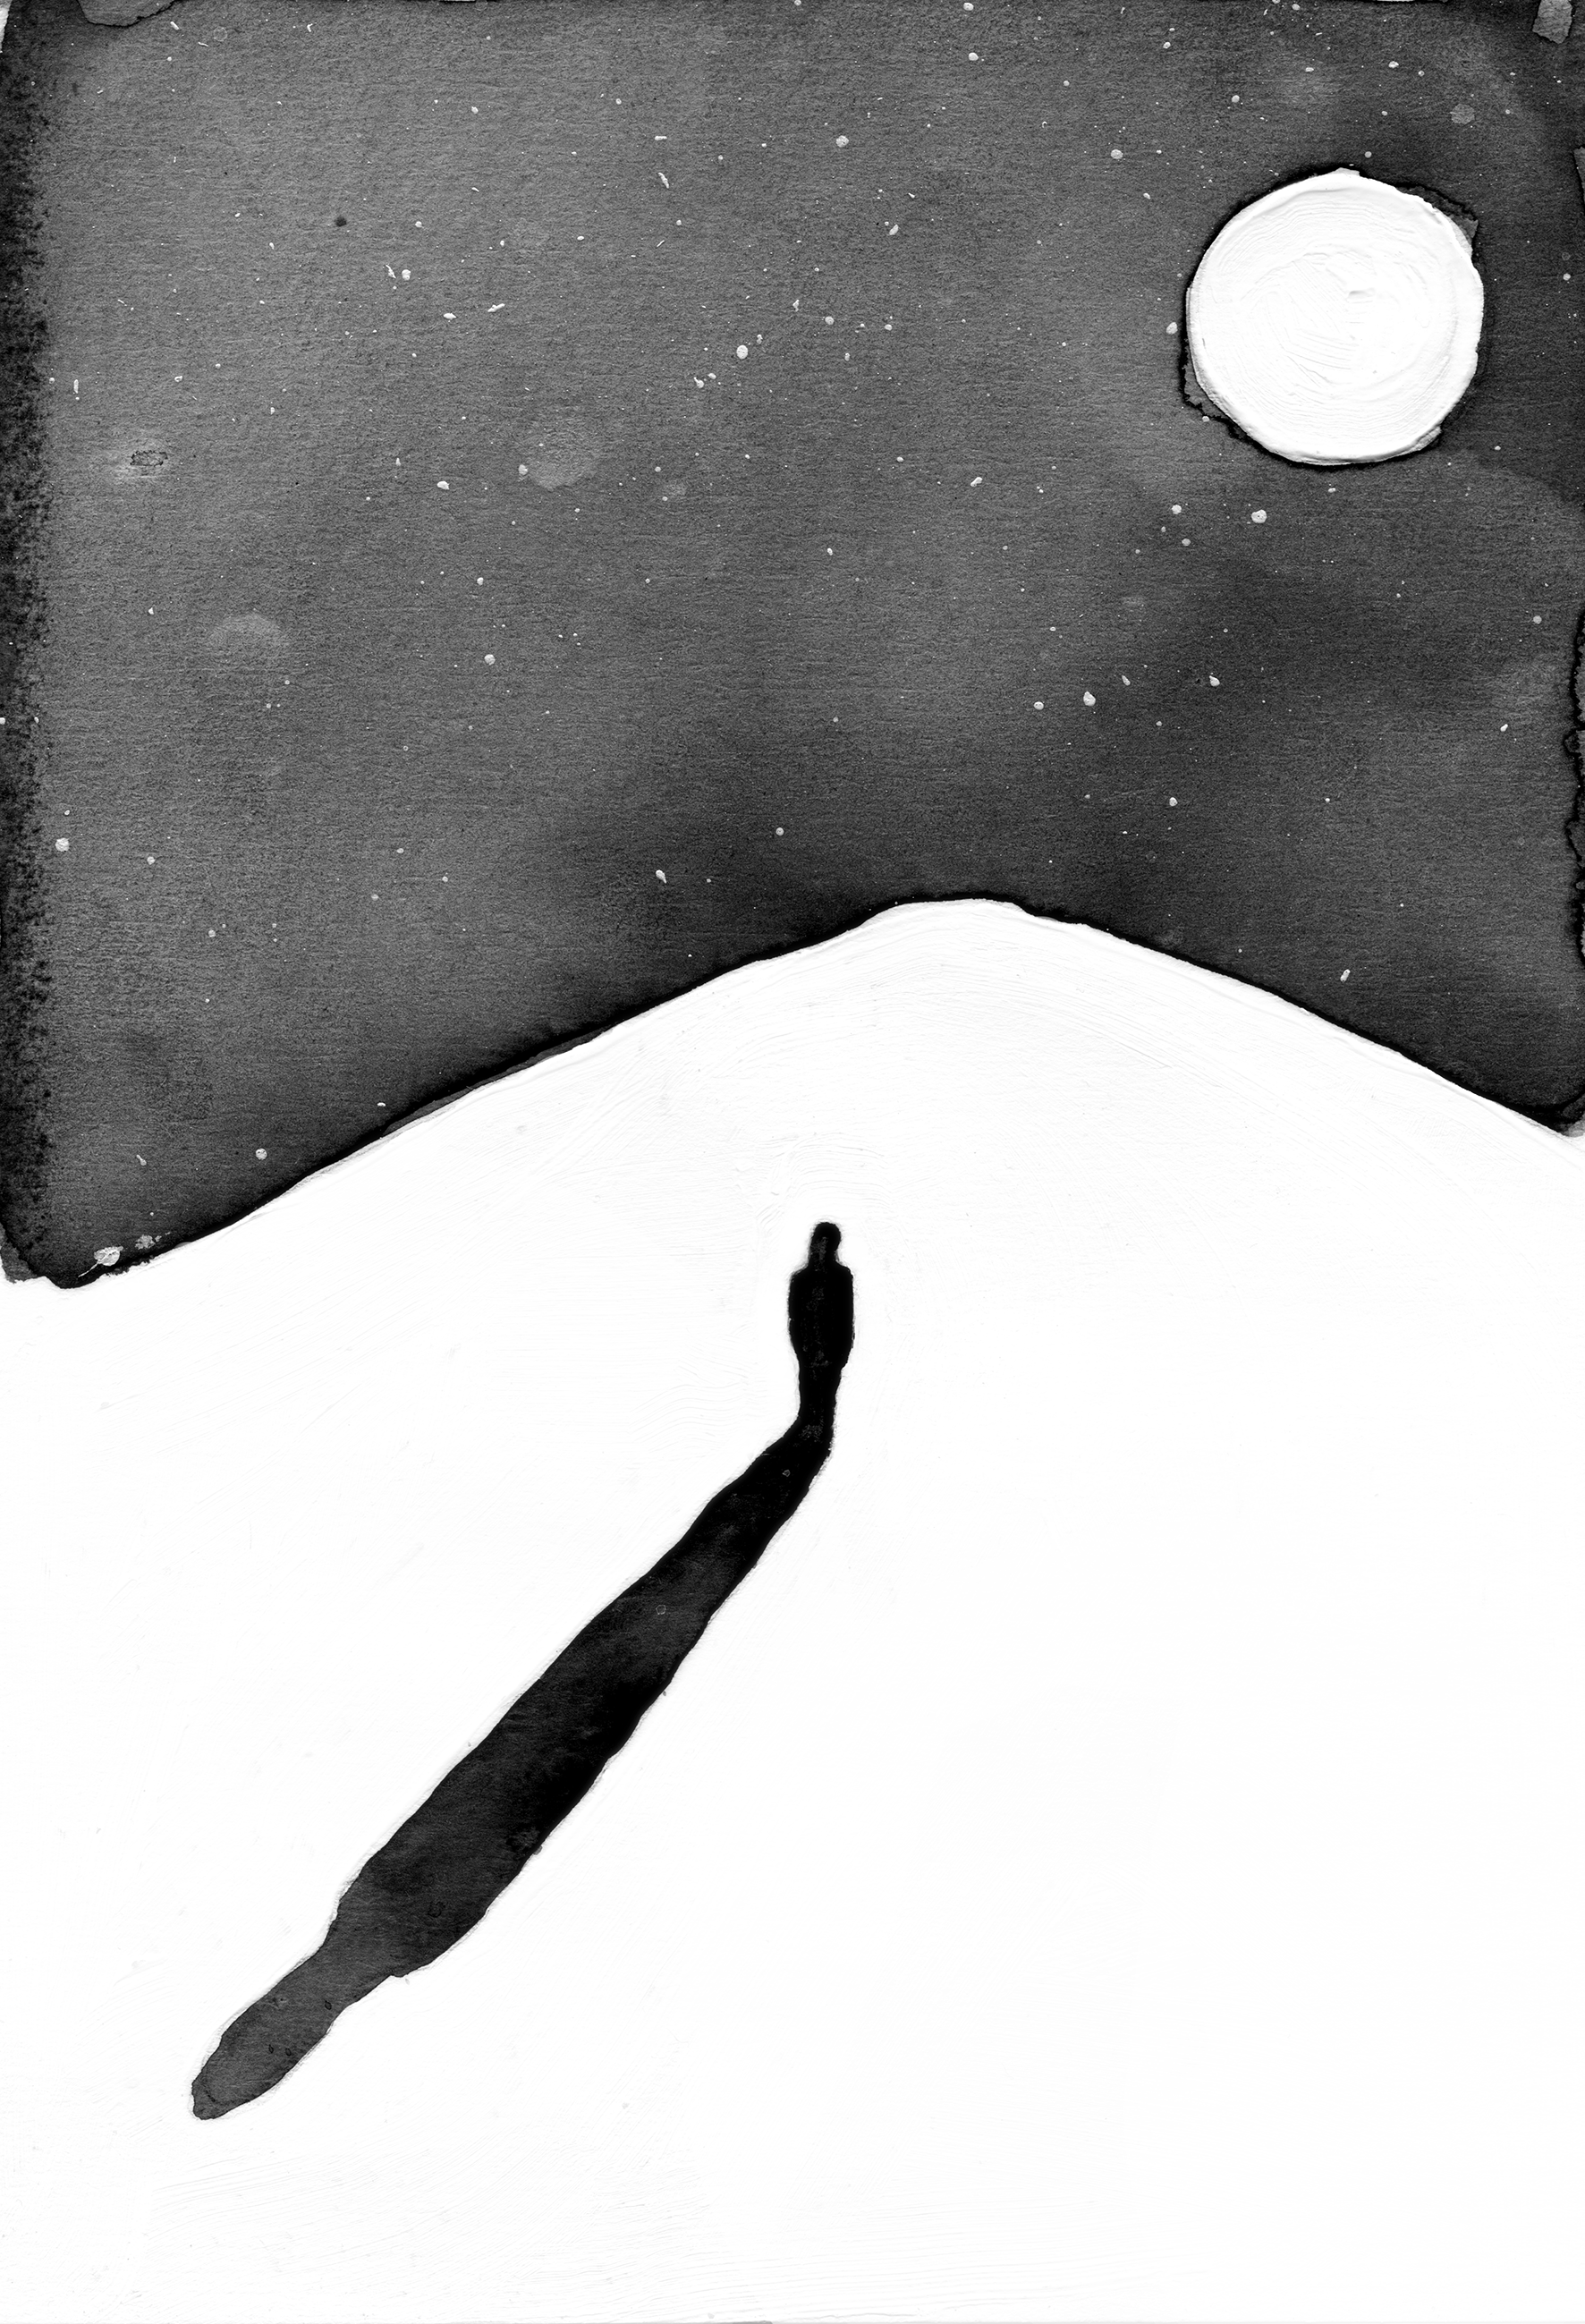
\includegraphics[width=155mm]{./imgs/9.pdf}
\end{figure}

\chapter{As gralhas}

Num domingo, jogavam baralho na ala dos criados: Vassíli --- um
trabalhador ---, Michka Koriachónok, Lióksia --- ajudante de pastor ---
e Artiom --- um mujique altíssimo, curvado e de pernas compridas e
arqueadas. Artiom era um homem sem"-terra e sem cavalo, passara a vida na
lavoura e sempre tivera vontade de casar, mas as moças não se
interessavam por ele. Fazia dias que observava Dúnia, uma jovem corada,
bonita, que cuidava do leite. Ela corria o dia todo dos estábulos para a
casinha da adega ou para a cozinha, ressoava com baldes de zinco,
exalava sempre cheiro bom de leite fresco e, quando nevava, flocos caíam
chiando em suas bochechas. Ela era uma moça risonha. Artiom, seja lá o
que estivesse fazendo --- tirando a moinha da eira ou limpando a
manjedoura das ovelhas ---, ao ver Dúnia, fincava o forcado e ia atrás
dela andando com as pernas compridas feito um camelo. Ao aproximar"-se,
tirava o chapéu e a cumprimentava, inclinando a cabeça:

--- Bom dia, Dúnia.

--- Bom dia --- ela apoiava os baldes no chão e tapava a boca com o
avental.

--- Sempre cuida do leite, Dúnia?

Nesse momento, ela se abaixava, impotente pelo cômico da situação,
pegava os baldes e corria por uma estradinha coberta de neve até a
casinha da adega, então largava os baldes com força no chão e logo ia
dizendo à governanta Vassilissa: ``Minha cara, esse camelo de novo me
pediu para casar com ele, acho que eu morreria!'' --- e ria tão alto que
dava para ouvir no quintal todo.

Nikita foi à ala dos criados. Como nesse dia cozinhavam sopa de cabeça
de carneiro, sentia"-se um cheiro agradável de carne de carneiro e também
de pão assado. Junto à porta de entrada, onde sobre uma tina penduravam
a jarra de barro do lavatório, acumulara"-se neve úmida trazida
da rua. Num banco perto da estufa estava sentado Pakhom, cujos cabelos
pretos caíam na testa bexiguenta e nas sobrancelhas zangadas. Ele
remendava o cano de sua bota: furava cuidadosamente o couro com um
furador, levando a cabeça para trás, semicerrava os olhos, enfiava uma
cerda de porco na ponta do linhol, transpassava o furo com ela e,
apertando o cano entre os joelhos, puxava a linha pelas duas pontas.
Olhou enviesado para Nikita, por debaixo das sobrancelhas: brigara com a
cozinheira e estava zangado --- em vez de secar, ela queimara os panos
para enrolar nos pés.

Os jogadores, por ser domingo, estavam à mesa de camisa limpa e cabelos
penteados com óleo. Somente Artiom estava desgrenhado e vestia um cafetã
furado: não havia ninguém que cuidasse dele e lavasse suas camisas. Os
homens produziam estalidos com as cartas pegajosas e mal cheirosas e
diziam:

--- Cubro e aposto mais dez.

--- Cubro e aposto mais cinquenta.

--- Viu isso?

--- E você, viu?

--- Sabichão!

--- Ah!

--- Então, Artiom, aguente essa!

--- Como assim? --- dizia Artiom, olhando surpreso para as cartas. ---
Não está certo, é um erro.

--- Mostre o nariz.

Artiom pegou uma carta em cada mão e cobriu os olhos com elas.

O trabalhador Vassíli, hesitante, começou a bater com três cartas no
nariz comprido dele. Os outros jogadores olhavam, contavam as
pancadinhas no nariz e gritavam bravamente para que Artiom não se
mexesse.

Nikita sentou"-se para jogar e imediatamente perdeu --- aplicaram"-lhe
quinze cartas no nariz. Nesse instante, Pakhom, colocando a bota e a
ferramenta de sapateiro embaixo do banco, disse severamente:

--- Enquanto uns devem estar voltando da missa, estes nem fizeram o sinal
da cruz e já pegaram as cartas. Estão de olho na comida dos dias
gordos\ldots{} Stepanida --- gritou ele, levantando"-se e indo ao lavatório ---,
arrume o almoço!

A cozinheira, Stepanida, de susto deixou cair uma tampa de ferro na
cozinha. Os trabalhadores juntaram as cartas. Vassíli virou"-se para o
canto onde estava um ícone de papel com marcas de barata e fez o sinal
da cruz.

Stepanida entrou trazendo uma tigela de madeira com miolos de carneiros
da qual saía um vapor aromático que lhe cobria o rosto esquivado.
Os trabalhadores sentaram à mesa em silêncio, com expressão
séria, e pegaram as colheres. Vassíli começou a cortar o pão em fatias
compridas, distribuindo uma para cada, e bateu na tigela, dando sinal
para a refeição começar. Como era saborosa a sopa de cabeça de carneiro.

Pakhom não se sentou à mesa, somente pegou uma fatia de pão e voltou
para o banco perto da estufa. A cozinheira trouxe"-lhe batatas quentes e
um saleiro de madeira. Ele jejuava na quaresma.

--- Os panos para enrolar nos pés --- disse a ela Pakhom, partindo
cuidadosamente uma batata fumegante e mergulhando a metade dela no
saleiro ---, você queimou os panos de novo, mulher tola. Pois é\ldots{}

Nikita saiu para o quintal. O dia estava nublado. Soprava um vento úmido
e pesado. Sobre a neve cinzenta e grossa como sal transparecia esterco
amarelo. A estrada para trenós que dava no dique, coberta de estrume e de
poças, era mais alta que a neve ao redor. Os muros de troncos dos
quintais, os telhados de palha escurecidos, as árvores nuas, uma casa de
madeira sem pintura --- tudo era cinzento, escuro, perceptível.

Nikita foi até o dique. Ao longe se ouvia o ruído de árvores molhadas,
como se, em lugar distante, a água rumorejasse ao passar por comportas.
Os cumes oscilantes dos salgueiros estavam envolvidos por nuvens vazadas
e baixas. Nas nuvens, no meio de galhos trêmulos, pássaros pretos
ganhavam voo, rodopiavam, gritavam com vozes roucas e inquietas.

Nikita estava com a cabeça virada para o alto e a boca aberta. Aqueles
pássaros pareciam ter surgido do vento úmido e denso, como que trazidos
pelas nuvens, e, agarrando"-se aos salgueiros ruidosos, gritavam sobre
algo angustiante, assustador e alegre --- Nikita respirava com
dificuldade, seu coração batia acelerado.

Eram as gralhas que retornavam com a primeira tempestade da primavera
para seus antigos lares, para seus ninhos destruídos. Chegou a
primavera.

\chapter{A casinha sobre rodas}

Um vento úmido soprou durante três dias, engolindo a neve. Nos morros, a
terra arada com seus sulcos escuros foi descoberta. O ar cheirava a neve
derretida, a esterco e gado. Quando abriram os portões dos estábulos,
vacas saíram para o poço, empurrando"-se, tocando"-se com os chifres e
mugindo alto. O touro Baian urrava ferozmente, farejando o vento da
primavera. Michka Koriachónok e Lióksia, cada um com um chicote, a muito
custo conseguiram colocar o gado de volta nos estábulos entulhados de
esterco. Abriram os portões do curral, e cavalos de pelo escurecido e
desbotado, de crinas sujas e caídas e barrigas inchadas, saíram
sonolentos, como bêbados. A égua Viesta estava parindo na baia ao lado
da estribaria. Gralhas molhadas voavam sem rumo, agitando"-se e gritando
sobre os telhados. Nos fundos, atrás da casinha da adega, corvos
circundavam uma carniça surgida debaixo da neve. Árvores farfalhavam com
ruídos pesados e inquietantes. Sobre o dique, entre nuvens e salgueiros,
gralhas voavam crocitando.

Nikita, durante esses dias, esteve com dor de cabeça. Sonolento, aflito,
ele vagava pelo quintal, por estradas alagadas, ia até a eira, onde as
pilhas de moinha cheiravam a poeira de cereais e a ratos. Ele se sentia
perturbado e inquieto, como se algo terrível estivesse para acontecer,
algo que não poderia ser compreendido nem perdoado. Tudo para ele --- a terra, os
animais, o gado, os pássaros --- parou de ser compreensível e familiar
e se tornou alheio, hostil, ameaçador. Algo aconteceria,
algo incompreensível e pecaminoso, e aconteceria sem falta. Mesmo assim,
mesmo sonolento e atordoado pelo vento, pelo cheiro de carniça, de
cascos de cavalos, de esterco e neve fofa, ele era tomado por uma
curiosidade que o atraía a tudo isso.

Quando voltou para casa, molhado, parecendo um selvagem e cheirando a
cachorro, a mãezinha olhou fixamente para ele com repreensão e sem
afeto. Nikita não entendeu por que ela ficara zangada e isso o
perturbava ainda mais, fazendo"-o sofrer. Nos últimos dias, ele não tinha
feito nada de errado, mas se sentia ansioso como se fosse culpado de
algum grande pecado que, sem motivo aparente, varria a terra inteira.

Nikita andava ao longo de uma meda, do lado protegido do vento. Nessa
meda ainda se distinguiam os espaços cavados por trabalhadores e moças
no outono tardio, quando debulharam os últimos amontoados de trigo. De
noite entravam nas cavidades, no fundo da meda, para dormir. Nikita se
lembrou das conversas que ouvia lá, na escuridão da palha quente e
cheirosa. A meda agora lhe parecia terrível.

Ele aproximou"-se de um casebre de lavrador perto da eira, no
campo --- uma casinha de tábuas sobre rodas. A porta balançava, presa a
uma dobradiça, e rangia desanimadamente. A casinha estava vazia. Nikita
entrou por uma escadinha de cinco vigas. Dentro havia uma janelinha de
quatro vidraças. No chão ainda se via neve. Embaixo do telhado, numa
pequena prateleira na parede, foram largados uma colher roída de madeira
do outono passado, uma garrafa de óleo de cozinha e um cabo de faca. O
vento sibilava sobre o telhado. Ali parado, Nikita pensava que agora
estava completamente sozinho, que ninguém o amava e todos estavam
zangados com ele. Tudo no mundo era úmido, sombrio, sinistro. Seus olhos
encheram"-se de lágrimas e ele sentiu um amargor: e não era para menos,
sozinho neste mundo, num casebre abandonado\ldots{}

--- Senhor --- disse Nikita em voz baixa, sentindo um calafrio nas
costas ---, permita que tudo fique bem de novo. Que mamãe me ame, que eu
obedeça a Arkádi Ivánovitch\ldots{} Que o sol apareça, que a grama cresça\ldots{}
Que as gralhas não gritem tão assustadoras\ldots{} Que eu não ouça mais o
rugido do touro Baian\ldots{} Senhor, permita que eu me sinta leve de novo\ldots{}

Dizendo isso, Nikita curvou"-se e fez o sinal da cruz apressadamente. E,
depois de fazer sua prece, olhando para a colher, a garrafa e o cabo de
faca, ele de verdade se sentiu mais leve. Ainda ficou algum tempo no
casebre mal iluminado por uma janelinha e foi para casa.

Realmente a casinha ajudou: na antessala, enquanto Nikita tirava o
sobretudo, a mãezinha, de passagem, fixou nele os olhos sérios e
cinzentos, como passou a fazer nos últimos dias, mas repentinamente sorriu
com ternura, afagou o cabelo dele e disse:

--- Então, cansou de correr? Quer tomar chá?

\chapter{O aparecimento extraordinário\break de Vassíli Nikítievitch}

À noite, finalmente desabou a chuva, um temporal que começou a bater tão
forte na janela e no telhado de ferro que Nikita acordou, sentou"-se na
cama e se pôs a ouvir, sorrindo.

O maravilhoso ruído da chuva noturna. ``Dorme, dorme, dorme'' --- ela
tamborilava apressadamente nos vidros, e na escuridão o vento arrancava
com ímpeto os álamos diante da casa.

Nikita virou o lado frio do travesseiro para cima, deitou"-se de novo e
revirou"-se na cama debaixo do cobertor de tricô, acomodando"-se da melhor
maneira. ``Tudo será bom, terrivelmente bom'' --- pensava e se largava
nas nuvens macias e quentes do sono.

Perto do amanhecer a chuva passou, mas o céu ainda estava encoberto por
nuvens pesadas, voando de Sul a Norte. Nikita olhou pela janela e disse
um ``ah''. Da neve não sobrara rastro. O amplo quintal foi coberto de
poças encrespadas pelo vento. Sobre elas e sobre a relva cinzenta e
amassada, estendia"-se um caminho de esterco ainda não de todo consumido
pelas chuvas. Os galhos encharcados lilás dos álamos sacudiam, alegres e
ágeis. Ao Sul, por entre nuvens vazadas, apareceu uma nesga do céu azul
ofuscante voando para a propriedade com grande rapidez.

Durante o chá, a mãezinha estava nervosa e olhava a cada instante para
as janelas.

--- Hoje é o quinto dia sem correspondência --- disse ela a Arkádi
Ivánovitch ---, não estou entendendo nada\ldots{} Ele esperou tanto que
chegaram as enchentes do degelo e agora as estradas ficarão imprestáveis
por duas semanas\ldots{} Que imprudência terrível!

Nikita compreendeu que a mãezinha falava do pai --- ele era esperado a
qualquer momento. Arkádi Ivánovitch foi conversar com o administrador
--- não seria possível mandar alguém a cavalo buscar a correspondência?
---, mas no ato retornou para a sala de jantar e disse em voz alta e com
uma entonação incomum:

--- Senhores, vejam o que está acontecendo!\ldots{} Venham cá --- ouçam o
barulho das águas.

Nikita escancarou a porta que dava para a entrada. O ar limpo e
penetrante estava repleto de ruídos agudos e fortes de água se
precipitando. Uma enormidade de córregos oriundos da neve jorrava por
todos os sulcos, valetas e escoadouros em direção às ravinas. Cheias até
a borda, as ravinas mandavam as águas da primavera para o rio. Ao quebrar
o gelo, o rio transbordava revirando blocos de gelo e arbustos
arrancados pela raiz, depois passava por cima do dique e escorria em
torvelinho.

A nesga azul que voava para a propriedade se rompeu e dispersou as
nuvens de chuva, uma luz azul refrescante derramou"-se do céu, as poças
do quintal matizaram"-se de um azul sem fundo, os arroios ganharam
reflexos brilhantes, e as enormes lagoas dos campos e as ravinas
transbordantes refletiram o sol com feixes de luz.

--- Deus, que ar delicioso! --- disse a mãezinha, apertando as mãos
contra o peito, sob o xale de lã. Seu rosto sorria e nos olhos azuis
havia faíscas verdes. Ao sorrir, ela se tornava a mãe mais linda do
mundo.

Nikita andou ao redor do quintal para ver o que estava acontecendo lá.
Por toda parte corriam filetes de água enfiando"-se por vezes sob
amontoados de neve cinza granulada que desapareciam sob os pés. Não
importa para onde se olhava, por toda parte se via água: a propriedade
parecia uma ilha. Nikita conseguiu chegar somente até a ferraria, que
ficava num morro. Ele correu para a ravina pelo declive, que ia secando.
Amassando a relva do ano passado, a água vinda da neve, perfumada e
cristalina, fluía e jorrava. Ele pegou um punhado e tomou.

Adiante, o fundo da ravina ainda estava coberto de neve, com manchas
amarelas e azuis. A água ora rompia da neve numa torrente, ora corria
acima dela, formando, como ali se dizia, o \emph{naslus} --- Deus livre
qualquer um de passar a cavalo nessa mistura de neve e água. Nikita ia
acompanhando o fluxo da água: como seria bom nadar nessas águas
primaveris, de uma ravina à outra, diante de margens amolecidas que iam
secando, nadar através das lagoas luminosas e encrespadas pelo vento da
primavera.

Do outro lado da ravina ficava um campo plano --- em alguns lugares
cinza"-amarronzado, em outros ainda nevado --- que reluzia com os filetes
ondulados de água. Ao longe, através do campo, cinco cavaleiros sem sela
galopavam lentamente. O da frente virou"-se e aparentemente gritou alguma
coisa gesticulando com um maço de cordas. Pelo cavalo malhado Nikita
reconheceu Artamon Tiúrin. O homem detrás apoiava uma vara no ombro. Os
cavaleiros passaram correndo na direção da aldeia de Khomiakоvka, que
ficava do outro lado do rio, depois das ravinas. Tudo isso era muito
estranho --- mujiques galopando fora da estrada no meio da enchente.

Nikita foi até a lagoa de baixo, para onde fluía pela neve amarelada uma
larga cortina de água vinda da ravina. A água cobria o gelo da lagoa e
formava ondas baixinhas. À esquerda salgueiros rumorejavam, degelados,
vastos, enormes. Gralhas, que se molharam durante a noite, pousaram
oscilantes no meio de galhos nus.

Sobre o dique, entre troncos retorcidos, apareceu um cavaleiro.
Batia com os calcanhares em um cavalo franzino, cambaleava e levantava
os cotovelos. Era Stiopka Karnaúchkin: ele gritou algo para Nikita
enquanto galopava sobre as poças; torrões de neve suja e respingos de
água voavam por baixo dos cascos do cavalo.

Estava claro que algo acontecera. Nikita correu para casa. Perto da
entrada de serviço o cavalinho de Karnaúchkin, movendo os flancos
inchados, sacudiu o focinho para ele. Mal  Nikita irrompeu em casa, ouviu
um grito curto e terrível da mãezinha. Ela apareceu no fundo do
corredor, seu rosto estava transtornado e os olhos esbranquiçados e
arregalados de horror. Atrás dela apareceu Stiopka e, da porta ao lado,
saiu rapidamente Arkádi Ivánovitch. A mãezinha não andava, mas
voava pelo corredor.

--- Rápido, rápido --- gritou ela, escancarando a porta da cozinha ---,
Stepanida, Dúnia, corram para a ala dos criados!\ldots{} Vassíli Nikítievitch
está se afogando perto da aldeia de Khomiakovka\ldots{}

O mais terrível era que ele estava ``perto da aldeia de Khomiakovka''. A
vista de Nikita toldou: do corredor veio de repente cheiro de cebola
frita. A mãezinha depois passou a contar como Nikita nesse momento
cerrou os olhos e gritou feito uma lebre. Mas ele mesmo não se lembrava
desse grito. Arkádi Ivánovitch o agarrou e o puxou para o quarto de
estudar.

--- Você não tem vergonha, Nikita, já é um rapazinho crescido ---
repetia ele apertando com toda a força os braços de Nikita, logo acima
dos cotovelos. --- Não é nada, não é nada\ldots{} Vassíli Nikítievitch logo
chegará\ldots{} Claro que simplesmente caiu numa vala, se molhou\ldots{} E esse
idiota do Stiopka assustou a sua mãe\ldots{} Dou minha palavra, vou dar um
puxão de orelhas nele\ldots{}

Mesmo assim, Nikita viu como os lábios de Arkádi Ivánovitch estavam
tremendo, e as pupilas de seus olhos eram como pontinhos.

Enquanto isso, a mãezinha correu somente de vestido para a ala dos
criados, apesar de os trabalhadores já saberem de tudo, agitarem"-se
perto da cocheira, atrelarem com estardalhaço o garanhão Negro, um
cavalo bravo e forte, a um trenó sem patins de ferro e laçarem os
cavalos de montaria do curral. Alguém tirava um croque de cima do
telhado de palha; um corria com uma pá; outro trazia um maço de
cordas; Dúnia vinha depressa de casa abraçando casacos de pele de
carneiro --- um com gola e forro de pele e outrо com mangas de pele
dobradas para fora. Pakhom aproximou"-se da mãezinha:

--- Faça um esforço, Aleksandra Leóntievna, mande Dúnia para a aldeia
comprar vodca. Assim que o trouxerem, precisa dar vodca para ele\ldots{}

--- Pakhom, eu vou com o senhor.

--- De jeito nenhum, vá para casa, ainda pegará um resfriado.

Pakhom sentou de lado no trenó, pegando fortemente as rédeas.
``Soltem!'', gritou para os rapazes que seguravam o cavalo pelo bridão.
Negro se abaixou nos tirantes, bufou, deu um arranco e puxou com
facilidade o trenó sobre a lama e as poças de água. Atrás dele galopavam
os trabalhadores, gritando e fustigando os cavalos que queriam se
amontoar. A mãezinha olhou demoradamente na direção deles, abaixou a
cabeça e foi devagar para casa. Na sala de jantar, de onde podiam ver, do outro lado do morro, o campo e os salgueiros de Khomiakovka,
a mãezinha sentou"-se em frente à janela e chamou Nikita. Ele veio correndo,
abraçou"-a pelo pescoço e encostou"-se em seu ombro, no xale de lã\ldots{}

--- Deus não permitirá, querido Nikita, que a desgraça nos atinja ---
disse a mãezinha em voz baixa e nítida e ficou muito tempo com os lábios
encostados nos cabelos do filho.

Volta e meia Arkádi Ivánovitch aparecia no quarto, ajeitava os óculos,
esfregava as mãos. Volta e meia a mãezinha ia até a entrada, para ver se
não estavam vindo, e de novo se sentava diante da janela, sem deixar
Nikita se afastar.

A luz do dia já se tingia do lilás de antes do pôr do sol; os vidros das
janelas, na parte de baixo da esquadria, cobriram"-se de uma camada fina
de gelo: à noite ainda geava. E, de súbito, perto de casa, ouviu"-se um
tropel de cascos, e apareceram Negro, com a cara coberta de espuma, е
Pakhom, sentado de lado na boleia do trenó, e, no próprio trenó, debaixo
de uma pilha de diferentes peliças e um tapete de feltro, no meio de uma
pele de carneiro, surgiu o rosto corado e sorridente de Vassíli
Nikítievitch, com dois pingentes de gelo no lugar do bigode. A mãezinha
deu um grito e levantou"-se depressa --- o rosto dela tremia.

--- Está vivo! --- gritou ela, e lágrimas saltaram de seus olhos
radiantes.

\chapter{Como eu me afoguei}

No quarto, numa grande poltrona de couro encostada à mesa redonda,
sentava"-se o pai, Vassíli Nikítievitch, vestindo um penhoar macio de
pelo de camelo e calçados de feltro. O bigode e a barba castanha úmida
estavam penteados para os lados, o alegre rosto vermelho refletia"-se no
samovar, que de um jeito especial, como tudo nessa noite, fervia
ruidosamente e estalava com as faíscas da grelha de baixo.

Vassíli Nikítievitch semicerrou os olhos de prazer pela vodca tomada,
seus dentes brancos brilhavam. A mãezinha, apesar de estar com o mesmo
vestidinho cinza e o mesmo xale de lã, não se parecia com ela mesma ---
não podia conter o sorriso, os lábios franziam, o queixo tremia. Arkádi
Ivánovitch colocou os óculos novos de tartaruga que usava em ocasiões
especiais. Nikita se ajoelhou em cima de uma cadeira e, apoiando a
barriga na mesa, parecia entrar na boca do pai. A todo momento Dúnia
aparecia correndo, ora para pegar algo, ora para trazer algo, com os
olhos esbugalhados fixos no patrão. Stepanida trouxe numa frigideira de
ferro grandes panquecas, ``feitas às pressas'', que chiavam com manteiga
ao serem servidas --- de dar água na boca! O gato Vassíli Vassílievitch,
de rabo levantado, não parava de andar e de girar perto da poltrona de
couro, onde esfregava as costas, os flancos e a nuca: miau"-miau --- ele
cantava alto e com afetação. O ouriço Akhilka olhava com sua fuça de
porco por debaixo do bufê, seus espinhos achataram da testa às costas:
sinal de que também estava contente.

O pai comeu uma panqueca quente com prazer --- muito bem, Stepanida!
---, comeu outra enrolando"-a como um tubinho --- muito bem Stepanida!
---, sorveu um grande gole de chá com nata, endireitou o bigode e
semicerrou um olho.

--- Pois bem --- disse ele ---, agora vocês vão ouvir como me afoguei
--- e começou a contar. --- Eu saí anteontem de Samara. Aconteceu o
seguinte, Sacha --- por um instante ele ficou sério ---, surgiu uma
oportunidade muito vantajosa para mim: Pozdiúnin começou a me
importunar, queria porque queria que eu comprasse seu garanhão baio,
Lorde Byron. ``Para que'', disse eu, ``preciso de seu garanhão?'' ``Vá e
apenas olhe'', ele falou. Assim que vi o garanhão, fiquei apaixonado.
Uma beleza de cavalo. Esperto. Olhou de soslaio para mim com os olhos
lilás, como que dizendo --- compre"-me. E Pozdiúnin me importunando ---
``compre sem falta também o trenó e os arreios\ldots{}''. Sacha, você não
está zangada comigo por essa compra, não é? --- o pai pegou a mão da
mãezinha. --- Bem, vá, perdoe --- a mãezinha até fechou os olhos: será
que nesse dia ela tinha o direito de zangar"-se, mesmo que ele tivesse
comprado o próprio Pozdiúnin, presidente do \emph{zemstvo}?\footnote{\emph{Zemstvo},
  uma organização rural de administração local, criada em 1864, que
  cuidava de assuntos de educação, saúde, comércio, transporte,
  tecnologia agrícola, etc. Os cargos administrativos eram eletivos.}
--- Pois bem, eu mandei levar Lorde Byron para minha propriedade e
fiquei pensando no que fazer com ele. Não queria deixar o cavalo sozinho
em Samara. Coloquei na mala presentes diversos --- o pai semicerrou
maliciosamente um olho ---, de madrugada atrelaram Lorde Byron para mim,
e eu parti sozinho de Samara. No início ainda havia um pouco de neve em
alguns lugares, mas depois a estrada se tornou tão lamacenta que meu
garanhão ficou todo coberto de espuma e começou a tropeçar. Eu decidi
pernoitar em Koldyban, com o pope Vozdvijénski. O pope me ofereceu um
salame --- coisa de outro mundo! Pois bem. Ele me disse: ``Vassíli
Nikítievitch, não conseguirá chegar, verá por si só --- as ravinas sem
falta vão desabar de noite''. Mas eu queria viajar de qualquer jeito.
Assim fiquei discutindo com o pope até meia"-noite. Ele me serviu licor
de cassis! Palavra, se levassem tal licor para Paris, os franceses
perderiam a cabeça\ldots{} Bem, sobre isso falaremos depois. Assim que me
deitei, caiu um pé"-d'água. Imagine, Sacha, como fiquei desgostoso: estar
a vinte verstas\footnote{Versta (\emph{verstá}), medida russa de
  distância equivalente a 1,06 km.} de vocês sem saber quando
conseguiria encontrá"-los\ldots{} Ah, que esse pope e seu licor vão com
Deus\ldots{}

\begin{figure}
\vspace*{-2.65cm}
\hspace*{-2.85cm}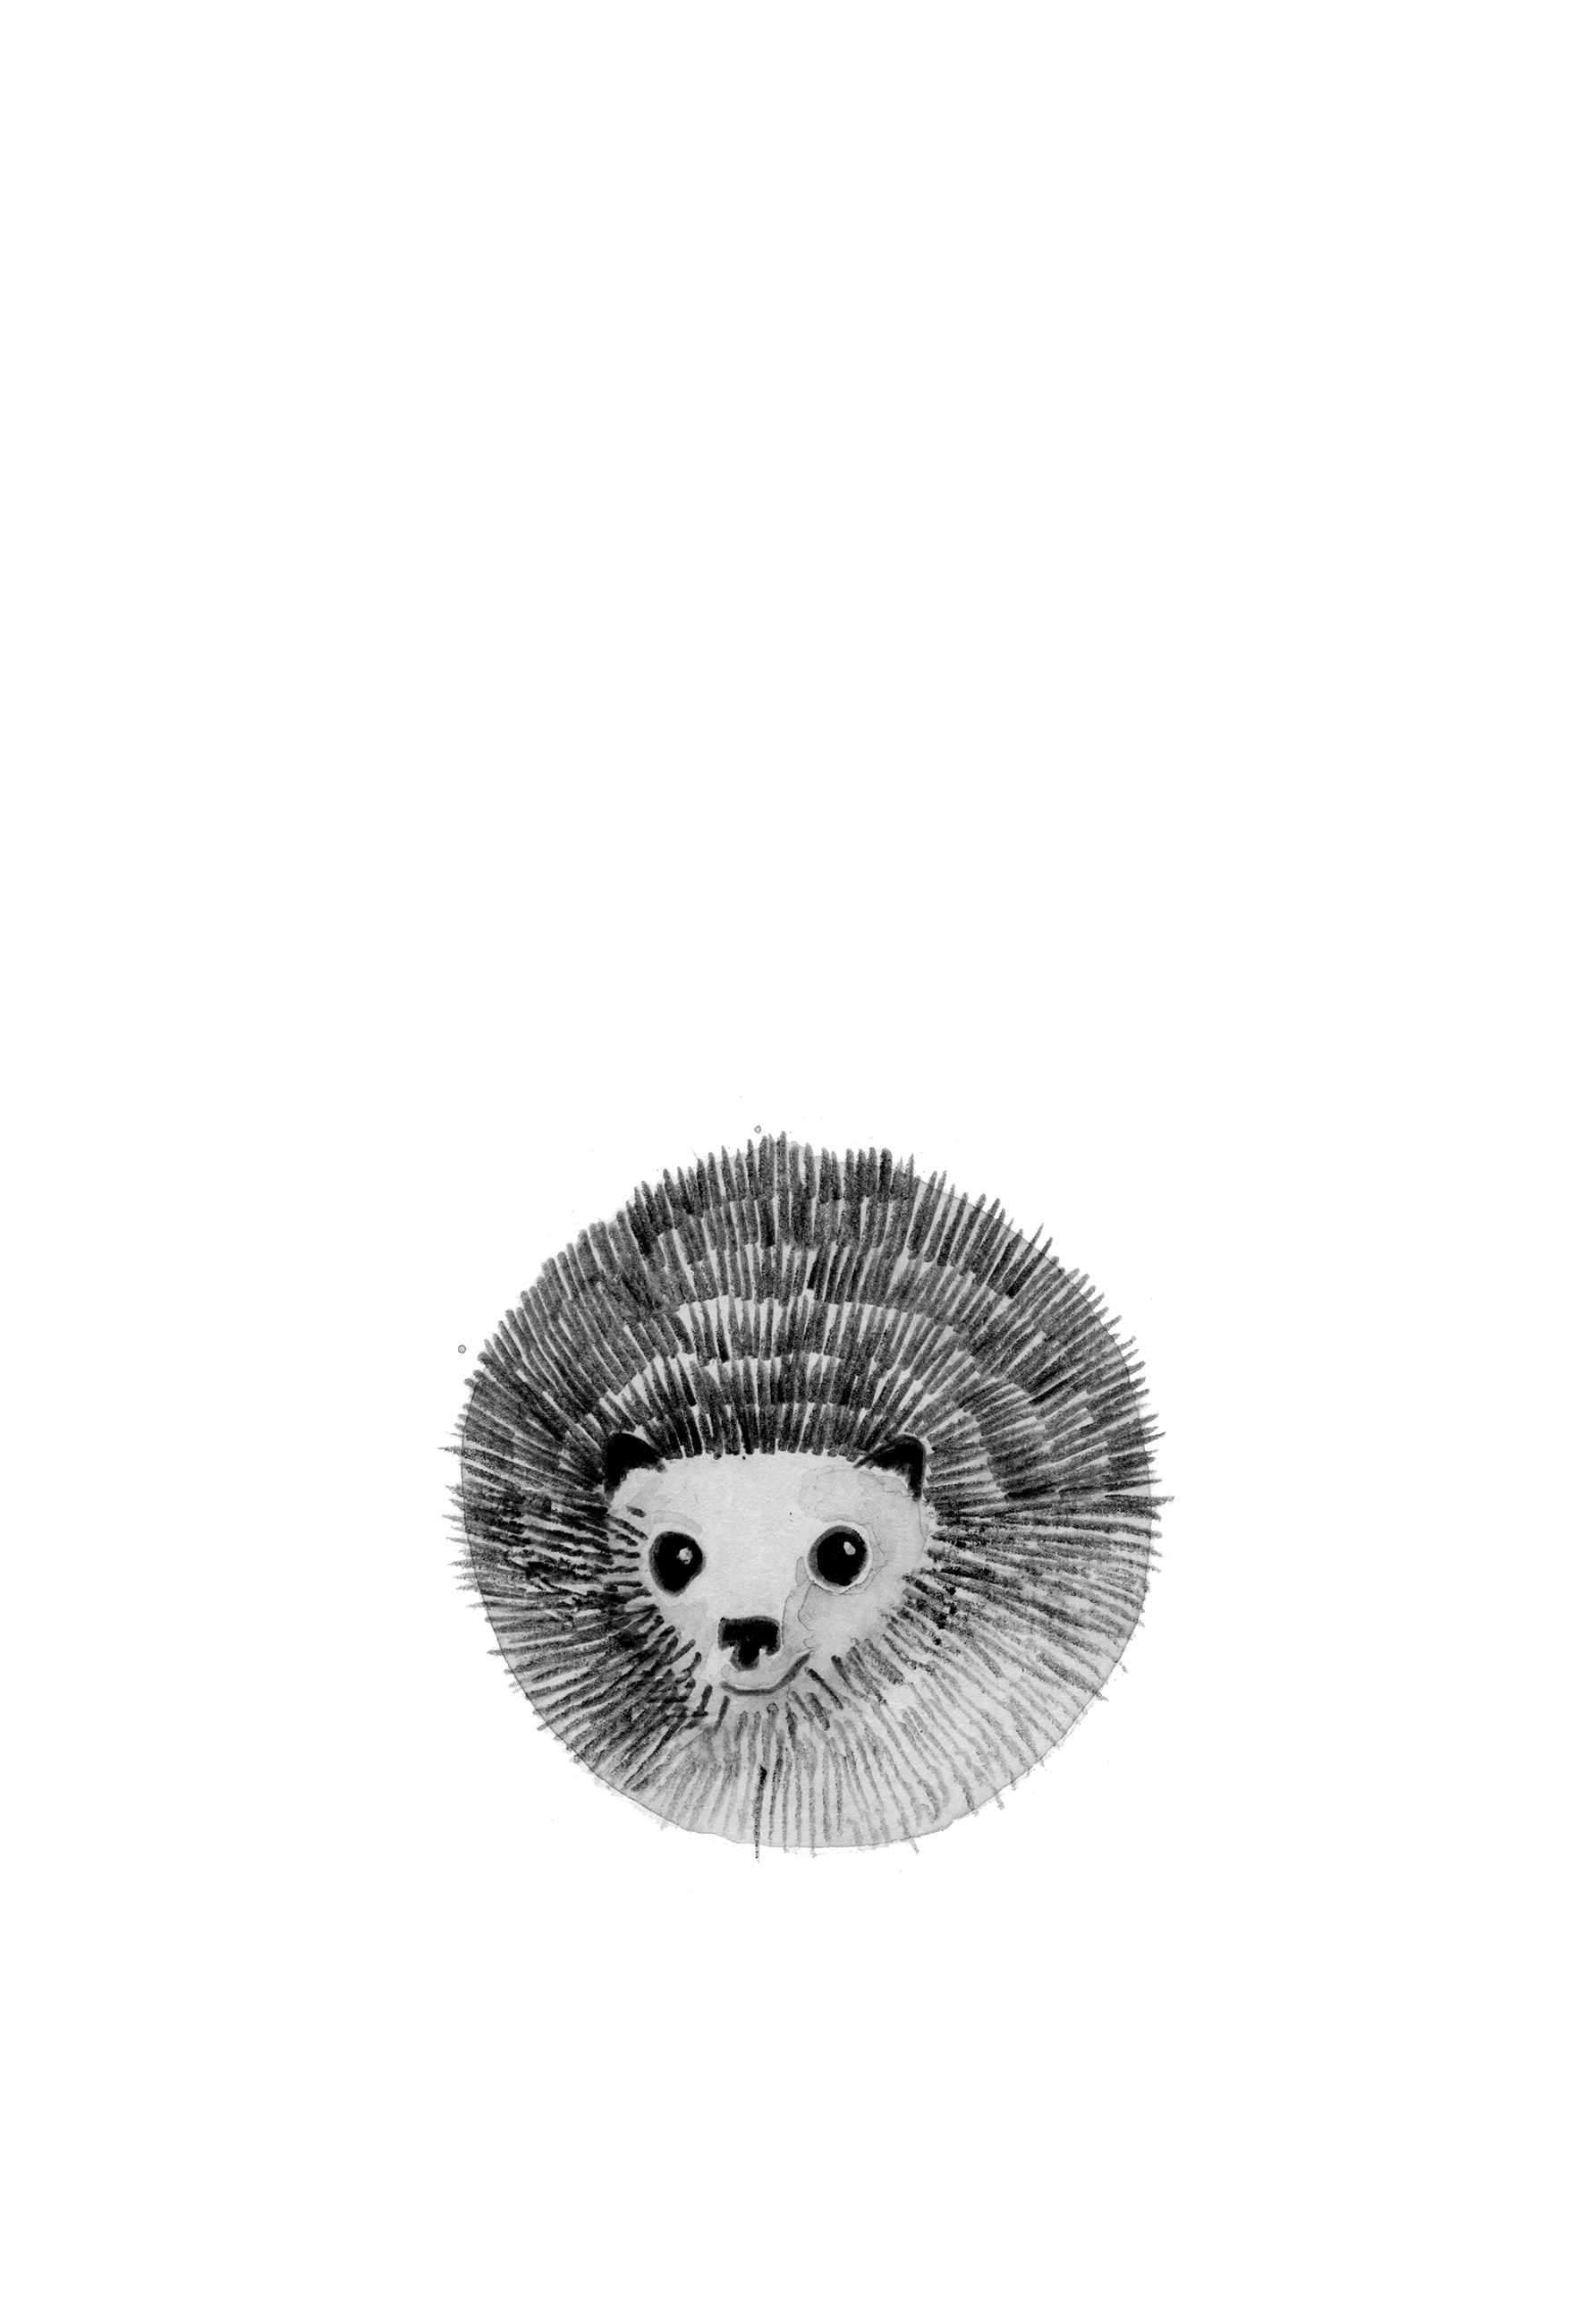
\includegraphics[width=155mm]{./imgs/5.pdf}
\end{figure}

--- Vassíli --- a mãezinha o interrompeu e olhou"-o com severidade ---,
peço seriamente que nunca mais se arrisque desse jeito\ldots{}

--- Você tem a minha palavra --- respondeu Vassíli Nikítievitch sem
hesitação. --- Pois bem, foi assim\ldots{} De manhã a chuvinha parou, o pope
foi à missa, eu mandei atrelar Lorde Byron e fui embora. Meu Pai!\ldots{} Ao
redor havia somente água. Mas para o garanhão ficou mais fácil. Nós
andávamos sem estrada, com a água até os joelhos, pelas lagoas\ldots{} Uma
beleza\ldots{} Sol, vento\ldots{} Meu trenó flutuava. Os pés se molharam. Eu me
sentia extraordinariamente bem! Finalmente vi de longe nossos
salgueiros. Aproximei"-me de Khomiakovka e comecei a experimentar onde
seria mais fácil atravessar o rio\ldots{} Ah, canalha! --- Vassíli
Nikítievitch bateu com o punho na mesa: --- Eu vou lhe mostrar, a esse
Pozdiúnin, onde se deve construir pontes! Fui obrigado a subir uma três
verstas acima de Khomiakovka e de lá atravessar o rio por um vau. O
valente Lorde Byron subiu rapidamente por uma margem íngreme. Bem,
pensei, o rio atravessamos, mas ainda temos três ravinas temerosas pela
frente. Mas eu já não tinha para onde ir. Aproximei"-me da primeira
ravina. Imagine, Sacha, o \emph{naslus,} toda aquela água misturada com
a neve nas margens. E a própria ravina, você bem sabe, tem umas três
braças de profundidade.

--- Que horror --- disse a mãezinha, empalidecendo.

--- Eu desatrelei o garanhão, tirei dele o peitoral e o cilhão e
coloquei"-os no trenó, só não pensei em tirar meu casaco de pele --- e
foi a minha ruína. Montei no Lorde Byron, que Deus o abençoe! O garanhão
no início refugou. Mas eu o acalmei, passando a mão nele. Ele farejou a
água e bufou. Deu marcha a ré e se jogou na ravina, direto no
\emph{naslus}. Afundou até o pescoço, lutava e não saía do lugar. Eu
desci dele e também afundei --- só a cabeça ficou de fora. Comecei a me
mover nesse lamaçal, ora nadando, ora me arrastando. E o garanhão,
percebendo que eu tinha saído de cima dele, relinchou queixosamente ---
não me abandone! ---, e começou a se debater e a saltar atrás de mim.
Alcançou"-me e bateu em minhas costas, no casaco aberto, com as patas da
frente, e me puxou para debaixo d'água. Debati"-me com todas as forças,
mas era empurrado mais e mais, e não havia fundo sob meus pés. A sorte
foi que o casaco estava aberto e, enquanto eu me debatia na água, ele
soltou"-se de mim. Deve estar lá no fundo da ravina\ldots{} Eu submergi,
respirei e fiquei estirado no lamaçal como uma rã, aí ouvi algo borbulhar.
Olhei para trás --- o garanhão tinha só metade da cara para fora e
soltava bolhas: ele tinha pisado no arreio. Eu tive que voltar. Soltei a
fivela, tirei o arreio. Ele ergueu a cabeça e olhou para mim com um
olhar humano. Assim ficamos, chafurdando no \emph{naslus} por mais ou
menos uma hora. Senti que não tinha mais forças, estava morrendo de
frio. O coração gelou. Nesse momento, percebi que o garanhão tinha
parado de saltar --- ele se virou e arrancou ---, então a muito custo
atingimos a água limpa. Ali o mais fácil seria boiar, e assim fomos
levados até a outra margem. Byron saiu primeiro para a relva, e eu fui
atrás. Peguei"-o pela crina e andamos lado ao lado --- ambos cambaleando.
Pela frente mais duas ravinas\ldots{} E, de repente, vi os mujiques
galopando\ldots{}

Vassíli Nikítievitch disse mais algumas palavras confusas e, de repente,
deixou tombar a cabeça. Seu rosto estava vermelho, os dentes batiam
rapidamente.

--- Não é nada, não é nada, estou apenas mole por causa do samovar ---
dizendo isso, encostou no respaldo da poltrona e fechou os olhos.

Começou a ter calafrios. Colocaram"-no na cama e ele passou a falar
disparates\ldots{}

\chapter{Semana Santa}

O pai ficou acamado por três dias com febre e, quando voltou a si, a
primeira coisa que fez foi perguntar se Lorde Byron ainda estava vivo. O
belo garanhão se achava com boa saúde.

O caráter vivo e alegre de Vassíli Nikítievitch logo o pôs de pé: não
era tempo de ficar de cama. Começava a agitação primaveril antes da
semeadura. Na ferraria, soldavam relhas, consertavam arados e colocavam
novas ferraduras nos cavalos. Nos celeiros, retiravam com pás o cereal
velho, incomodando os ratos e levantando uma nuvem de poeira. Sob o
alpendre, a tarara fazia ruído. Em casa, ocorria uma grande faxina:
limpavam janelas, lavavam pisos, tiravam teias de aranha dos tetos.
Levavam para a varanda tapetes, poltronas e sofás e com batidas
eliminavam o cheiro de inverno deles. Todas as coisas que tinham se
habituado a ficar em seus lugares no inverno foram importunadas, livres
de poeira, acomodadas de outro jeito. Akhilka, que não gostava de
agitação, de raiva foi morar na despensa.

A mãezinha limpava sozinha as baixelas de prata e as casulas de prata
dos ícones, abria os antigos baús, de onde vinha cheiro de naftalina, e
ali examinava as roupas de verão amassadas que, de tanto descansarem no
inverno, tornaram"-se novas. Na sala de jantar havia cestos com ovos
cozidos;\footnote{A Páscoa russa, mais popular no país que o Natal, está
  repleta de ritos e tradições. Uma delas são os ovos de galinha (e não
  de chocolate) pintados pelas crianças, que depois os distribuem.}
Nikita e Arkádi Ivánovitch, usando uma infusão de casca de cebola,
tingiam os ovos, que, depois de amarelos, eram embrulhados em papéis e
mergulhados em água fervente com vinagre; então os ovos, já com desenhos
coloridos, eram envernizados, dourados e prateados.

Na sexta"-feira, espalhou"-se por toda a casa cheiro de baunilha e
cardamomo --- começavam a assar os bolos com frutas e nozes. Para a
noite, sobre a cama da mãezinha, já descansavam debaixo de toalhas
limpas dez bolos de Páscoa, uns espichados, outros achatados.

Os dias dessa semana foram instáveis --- ora vinham nuvens escuras de
chuva e caíam grãozinhos de neve, ora a luz fresca da primavera jorrava
do céu limpo e profundamente azul, ora chegava uma tempestade de neve
molhada. De noite, as poças cobriam"-se de geada.

No sábado, a propriedade esvaziou: metade das pessoas da ala dos criados
e de casa foi para a vila Kolokoltsovka, a sete verstas de lá,
para ver as matinas.

A mãezinha, nesse dia, não estava se sentindo bem --- passara mal a
semana toda. O pai disse que iria dormir logo depois do jantar. Arkádi
Ivánovitch, que ficou dias a fio esperando uma carta de Samara que não
veio, estava trancado no seu quarto, sombrio como um corvo.

Propuseram a Nikita o seguinte: se quisesse ir para as matinas, deveria
procurar Artiom e pedir que atrelasse à charrete a égua Afrodite, que
tinha ferraduras nas quatro patas. Precisaria sair antes de anoitecer e
parar na casa de um velho amigo de Vassíli Nikítievitch, Piotr
Petróvitch Deviátov, que tinha uma mercearia em Kolokoltsovka. ``A
propósito, a casa dele está cheia de crianças, e você está sempre
sozinho, isso não faz bem'' --- disse a mãezinha.

Ao entardecer, Nikita sentou"-se numa charrete de duas rodas ao lado do
enorme Artiom, que usava uma faixa nova na cintura do seu cafetã furado.
Ele disse: ``Vamos lá, minha cara, dê uma força'', e a velha Afrodite de
pescoço caído e ancas largas partiu trotando devagar.

Passaram pelo quintal, diante da ferraria, atravessaram a ravina com água
até o tornozelo. Afrodite, por algum motivo, o tempo todo olhava para
trás, para Artiom, através dos tirantes da charrete.

A tarde azul se refletia em poças cobertas de gelo fino. Os cascos \enlargethispage{\baselineskip}
estalavam, a charrete chacoalhava. Artiom não dizia nada e, baixando o
nariz comprido, pensava no\,amor infeliz que sentia por Dúnia. Sobre uma
faixa pálida do pôr do sol,\,iluminava"-se\,uma\,estrela\,clara\,como\,um\,cristal\,de\,gelo.

\chapter{Os filhos de Piotr Petróvitch}

Uma lâmpada presa a um aro de ferro pendia do teto, e sua chama curta,
azul e fedorenta quase não iluminava o quarto. No chão, em dois colchões
de chita que infundiam um cheiro acolhedor à moradia e às crianças,
estavam deitados Nikita e os seis filhos de Piotr Petróvitch ---
Volódia, Kólia, Liochka, Lionka, o Chorão, e mais dois menorzinhos cujos
nomes não interessavam a ninguém.

Os maiores contavam histórias em voz baixa. Lionka, o Chorão, volta e
meia tomava uma bronca --- ora beliscavam"-lhe a orelha, ora puxavam"-lhe
os cabelos, para que parasse de choramingar. Os menores dormiam com os
narizes enfiados nos colchões.

A sétima criança de Piotr Petróvitch era uma menina, Anna, da mesma
idade de Nikita --- sardenta, com olhos redondos atentos como um
pássaro, tinha o narizinho escuro de sardas e nunca sorria. De
tempos em tempos ela vinha pelo corredor sem fazer ruído e aparecia na
porta do quarto. Então, um dos garotos dizia:

--- Anna, não entre, senão eu me levanto e vou atrás de você.

E ela desaparecia também sem fazer ruído. A casa estava em silêncio.

Piotr Petróvitch era estaroste da igreja e foi para o templo ainda antes
de clarear.

Maria Mirónovna, sua esposa, disse aos filhos:

--- Se fizerem barulho, levam um tabefe na cabeça\ldots{}

E deitou"-se para descansar antes das matinas. Os filhos também receberam
ordem de ficarem deitados, sem brincar. Liochka, com o rosto redondo e
os cabelos espetados e sem os dentes da frente, contava:

--- Na Páscoa passada, quando a gente brincou de montinhos,\footnote{Jogo
  dos montinhos (\emph{igrá v podkútchki}), brincadeira russa de Páscoa
  em que, conforme uma antiga versão, escondiam ovos em montes de palha que
  deveriam ser encontrados pelos participantes.} eu ganhei duzentos
ovos. Comi tanto que a barriga parecia que ia explodir.

Atrás da porta, temendo que Nikita acreditasse em Liochka, Anna disse:

--- É tudo mentira. Não acredite nele.

--- Juro por Deus, agora mesmo eu me levanto e vou atrás de você ---
ameaçou Liochka.

E atrás da porta se fez silêncio.

Volódia, o mais velho, um menino moreno de cabelos encaracolados, estava
de pernas cruzadas sobre o colchão e disse a Nikita:

--- Amanhã iremos ao campanário para repicar os sinos. Quando eu começo,
a torre inteira treme. Com a mão esquerda toco os sinos menores --- dim,
dim --- e com esta toco o maior --- bum. O sino maior pesa cem mil
\emph{puds}.\footnote{\emph{Pud,} medida de peso russa equivalente a
  16,3 kg.}

--- É tudo mentira --- alguém sussurrou atrás da porta.

Volódia virou"-se tão rapidamente que até seus cachos se levantaram.

--- Anna!\ldots{} Nosso pai é forte à beça --- disse ele ---, consegue
levantar um cavalo pelas patas da frente\ldots{} Claro que eu ainda não
consigo, em compensação no verão, Nikita, você virá nos visitar e iremos
até a lagoa. Nossa lagoa tem seis verstas. Eu consigo subir até o topo
de uma árvore e de lá pular de cabeça dentro da água.

--- E eu consigo --- disse Liochka --- ficar sem respirar debaixo d'água
enxergando tudo. No verão passado a gente estava nadando, daí apareceram
minhocas e pulgas na minha cabeça, e besouros --- desse tamanho aqui\ldots{}

--- É tudo mentira --- alguém suspirou quase inaudível atrás da porta.

--- Anna, vou puxar as suas tranças!\ldots{}

--- Que menina irritante --- disse Volódia, aborrecido ---, está sempre
se intrometendo, só faz nos chatear, depois vai se queixar para nossa
mãe e dizer que estamos batendo nela.

Atrás da porta alguém choramingou. O terceiro menino, Kólia, deitado de
lado e escorando"-se no punho, olhava o tempo todo para Nikita com olhos
bondosos e um pouco tristes. O rosto dele era comprido e modesto, com
uma distância grande entre a ponta do nariz e o lábio superior. Quando
Nikita se virava para ele, Kólia sorria com os olhos.

--- Você sabe nadar? --- perguntou Nikita.

Kólia sorriu com os olhos. E Volódia disse com desdém:

--- Ele só fica lendo livros. No verão mora no telhado, numa
choupana; é uma choupana que fica no telhado. Fica lá deitado, lendo.
Nosso pai quer mandá"-lo estudar na cidade. E eu vou cuidar dos assuntos
de casa. Liochka ainda é pequeno, pode correr por aí. Nossa desgraça é o
Chorão --- ele puxou Lionka pelo topete de galo que tinha no cocuruto
---, é um menino tão enjoado. Nosso pai diz que ele tem vermes.

--- Ele não tem coisa nenhuma, eu é que tenho vermes terríveis --- disse
Liochka ---, porque como folhas de bardana e vagens de acácia, e posso
comer até girinos.

--- É tudo mentiria --- de novo alguém gemeu atrás da porta.

--- Eu avisei, Anna, agora aguente --- e Liochka voou do colchão até a
porta, empurrando um dos bebês, que, sem acordar, choramingou. Mas como
uma folha ao vento Anna desapareceu pelo corredor, sem deixar vestígio,
e ao longe apenas se ouviu o ranger da porta. Liоchka disse, retornando:
--- Foi se esconder com a mãe. Mesmo assim, não escapa: vai levar um
castigo.

--- Deixe"-a em paz, Liochka --- disse Kólia ---, por que ficam atrás dela?

Nesse momento, Liochka, Volódia e até Liоnka, o Chorão, ralharam com
ele:

--- Nós não ficamos atrás dela! Ela é que fica atrás de nós. Se
corrêssemos mil verstas de distância e nos virássemos, lá estaria ela,
sem falta, atrás de nós\ldots{} E tudo para ela é insuportável --- quando
alguém diz uma mentira, quando faz o que é proibido\ldots{}

Liochka disse:

--- Eu uma vez fiquei um dia inteiro dentro d'água, nas moitas de junco,
somente para não vê"-la --- fui todo comido por sanguessugas.

Volódia disse:

--- Basta nos sentarmos para o almoço e ela começa a nos dedurar para a
mãe: ``Mamãe, Volódia pegou um ratinho, está no bolso dele''. Mas pode
ser que para mim esse ratinho seja a coisa mais valiosa do mundo.

Lionka, o Chorão, disse:

--- Sempre fica encarando, olha para você até você começar a chorar.

Ao se queixarem de Anna a Nikita, os garotos esqueceram"-se completamente
de que a ordem era ficar em silêncio, não conversar antes das matinas.
De repente, ao longe se ouviu a voz grossa e ameaçadora de Maria
Mirónovna:

--- Será que devo repetir mil vezes?\ldots{}

Os garotos imediatamente se calaram. Depois, sussurrando, empurrando"-se,
começaram a calçar as botas, vestiram peliças curtas, enrolaram
cachecóis no pescoço e correram para a rua.

Maria Mirónovna apareceu de casaco novo de pelúcia e xale estampado com
rosas. Anna, enrolada em um grande lenço, segurava a mão de sua mãe.

A noite estava estrelada. Cheirava a terra e a frio. Ao longo de uma
fila de isbás escuras, andavam em silêncio: camponesas, mujiques e
crianças pisavam sobre poças congeladas que estalavam sob seus pés e
refletiam as estrelas. Ao longe, na praça da feira, contra o céu escuro,
destacava"-se a cúpula dourada da igreja. Sob ela, viam"-se lamparinas
acesas em três camadas. Um ventinho soprava e acariciava suas pequenas
chamas.

\chapter{Firmeza de espírito}

Depois das matinas voltaram para casa, onde a mesa já estava posta e
decorada com rosas vermelhas de papel espalhadas entre os bolos e doces
de Páscoa e fixas no papel de parede. Um canário piava na gaiola, no vão
da janela, incomodado pela luz da lâmpada. Piotr Petróvitch, de
sobrecasaca comprida, sorrindo atrás do bigode tártaro --- como era
costume dele ---, serviu um cálice de licor de ginja a cada um. As
crianças, descascando ovos, lambiam as colheres. Maria Mirónovna, sem
tirar o xale, sentava"-se, tão cansada que nem podia tomar o desjejum,
somente esperava que a turma --- assim ela chamava os filhos ---
finalmente sossegasse.

Assim que Nikita se deitou no colchão debaixo da chama azul da lâmpada e
se cobriu com a peliça de pele de carneiro, em seus ouvidos soaram vozes
finas e frias: ``Jesus Cristo ressuscitou dos mortos, com a morte
reparou a morte\ldots{}''. E ele de novo viu as paredes de tábuas
brancas, pelas quais escorriam lágrimas, e as luzes de muitas velas
diante das casulas douradas, e distinguiu através das nuvens de incenso,
lá no alto, sob a cúpula azul da igreja com estrelas douradas, um pombo
de asas estendidas. Do outro lado das janelas gradeadas estava noite,
vozes cantavam, sentia"-se cheiro de pele de ovelha e de tecido de
algodão vermelho, luzes de velas refletiam"-se em milhares de olhinhos,
então as portas do lado oeste se abriram, e bandeiras com imagens de
santos, inclinando"-se, começaram a marcha. Tudo o que tinham feito de
ruim no ano seria perdoado nessa noite. Anna, com o narizinho sardento e
dois laços azul"-claros sobre as orelhas, tentava beijar os irmãos\ldots{}

O dia seguinte amanheceu cinzento e quente. Todos os sinos repicavam.
Nikita e os filhos de Piotr Petróvitch, mesmo os menores, foram ao
celeiro da aldeia que ficava em frente ao curral. Lá, o povo reunido
deixava tudo colorido e barulhento. Garotos se entretinham com o jogo do
tentilhão e o jogo dos pinos, \footnote{No jogo do tentilhão (\emph{igrá
  v ``tchíjika'')}, antiga brincadeira russa, há um pauzinho afiado dos
  dois lados, o ``tentilhão'', que, fincado num burаquinho do campo,
  deve ser arremessado pelo jogador com um bastão, e o adversário tenta
  rebater. No jogo dos pinos (\emph{igrá v} \emph{tchúchki} ou \emph{v
  gorodki}), lembrando o boliche, o jogador, arremessando um bastão,
  precisa derrubar pinos de madeira dispostos de formas variadas.}
montavam uns nas costas dos outros. As moças ficavam sentadas em toras,
junto à parede do celeiro, usando xales coloridos sobre vestidos de
chita novos e mal ajustados ao corpo. Cada uma tinha na mão um lencinho
com sementes de girassol, uvas"-passas, ovos. Petiscavam, olhavam ao
redor maliciosamente e sorriam.

O sedutor Pietka, filho de estaroste, estava debruçado sobre os troncos
do outro lado, com as pernas esticadas e botas de salto nos pés; sem
fixar os olhos em ninguém, tirava sons do acordeão, atacando de repente:
``Ah, por que tu, por que tu\ldots{}''.

Perto de outra parede, formaram uma roda para jogar cara ou coroa, e
cada jogador tinha na mão uma pilha de moedas de dois e três
copeques. O lançador da vez derrubava uma moeda de cinco copeques no
chão, pisava nela, esfregando"-a com a sola da bota, depois a apanhava e
a arremessava para o alto: cara ou coroa?

Ali mesmo na terra, sobre a relva do ano passado, onde crescia cegueira
noturna,\footnote{Cegueira noturna (botão"-de"-ouro), tipo de ranúnculo
  que irrita os olhos, causando cegueira temporária.} as moças estavam
sentadas e jogavam o jogo dos montinhos: esconderam dois ovos nos montes
de uma parte da moinha e na outra parte nenhum: agora adivinhe onde
estão!

Nikita aproximou"-se dos montes de moinha e tirou um ovo do bolso, mas
Anna, que surgiu a tempo não se sabe de onde, sussurrou"-lhe atrás da
orelha:

--- Escute, não jogue com elas, vão enganar você e ganhar.

Anna fitou Nikita com os olhos redondos, sem sorrir, e fungou com o
nariz sardento. Ele foi até os garotos que brincavam de jogo dos pinos,
mas Anna apareceu de novo, vinda de algum lugar, e de canto de boca
sussurrou:

--- Não jogue com eles, querem enganar você, eu os escutei.

Não importa onde Nikita fosse, Anna corria atrás dele, como uma folha ao
vento, e sussurrava em seu ouvido. Ele não entendia por que ela estava
fazendo isso. Sentiu"-se incomodado e envergonhado, viu que os garotos
começaram a rir e um deles gritou com os olhos fitos nele:

--- Grudou na namoradinha!

Nikita foi até a lagoa, azul e fria. No fundo do barranco ainda havia
neve suja derretendo. Lá longe, sobre as árvores altas e nuas do
arvoredo, gralhas gritavam\ldots{}

--- Escute --- de novo sussurrava Anna às suas costas ---, eu sei onde
mora o esquilo"-do"-campo, se quiser, podemos vê"-lo.

Nikita, sem se virar, acenou negativamente com a cabeça, irritado. Anna
de novo sussurrou:

--- Juro por Deus, que um raio caia sobre minha cabeça se estou
enganando você. Por que não quer ver o esquilo?

--- Eu não vou.

--- Tá, então vamos colher cegueira noturna e depois esfregamos a
florzinha nos olhos e não vamos ver nada.

--- Não quero.

--- Então não quer brincar comigo?

Anna apertou os lábios, olhou para a lagoa, para suas águas azuis
onduladas, uma brisa deslocava para o lado sua trancinha apertada, a
ponta de seu nariz gracioso e sardento ficou vermelha, os olhos se
encheram de lágrimas, e ela piscou. E então Nikita compreendeu tudo:
Anna correu atrás dele a manhã toda porque sentia por ele o mesmo que
ele sentia por Lília.

Nikita foi rapidamente até a beira do barranco. Se Anna fosse atrás
dele, ele mergulharia na lagoa, de tanta vergonha e embaraço. Não podia
trocar com ninguém aquelas palavras estranhas, aqueles olhares e
sorrisos expressivos --- a não ser com Lília. Com qualquer outra menina
seria uma traição e uma vergonha.

--- Foram os meninos que falaram mal de mim --- disse ela ---, vou
contar tudo para mamãe\ldots{} Vou brincar sozinha\ldots{} Não preciso de
ninguém\ldots{} Eu sei onde fica uma coisa\ldots{} E é uma coisa muito
divertida\ldots{}

Nikita ouvia Anna resmungar, mas não lhe dava atenção, nem sequer se
virou para ela. O coração dele estava endurecido.

\chapter{Primavera}

Não era possível olhar para o sol, pois ele jorrava das alturas uma
torrente de luzes ofuscantes e desordenadas. Pelo céu azul profundo
pairavam nuvens lembrando montes de neve. A brisa primaveril cheirava a
relva fresca e a ninhos de pássaros.

Diante de casa botões eclodiam nos álamos perfumados, as galinhas
gemiam, aquecidas pelo sol. No jardim, a relva saía de dentro da terra
aquecida perfurando com tufos verdes as folhas podres, todo o prado
cobriu"-se de estrelinhas brancas e amarelas. A cada dia que passava,
aumentava o número de pássaros no jardim. Entre os troncos, começaram a
correr melros pretos, que ficavam em pé com habilidade. No meio das
tílias apareceu um papa"-figo, um pássaro grande, verde, com asas de
penugem amarelo"-ouro --- ele se agitava e assobiava com voz melosa.

Assim que o sol se erguia, os estorninhos acordavam e cantavam com
diferentes tons em todos os telhados e em suas casinhas, ora rouquejavam
e assobiavam como os rouxinóis, ora como as cotovias, ora como os
pássaros africanos que tinham ouvido no inverno, do outro lado do mundo
--- imitavam com zombaria e vozes dissonantes. Um pica"-pau passou voando
como um lencinho cinza através das bétulas\footnote{Bétula (\emph{berioza}), árvore com o caule de casca branco"-prateada que é um símbolo nacional na Rússia, assim como o abeto, principal conífera usada no Natal.} transparentes, pousou num
tronco, olhando para os lados e levantando a crista vermelha.

Numa manhã ensolarada de domingo, nas árvores ainda molhadas de orvalho,
um cuco piava à beira da lagoa, e com a voz triste, solitária e terna
abençoava a todos que moravam no jardim, começando pelas minhocas:

--- Vivam, amem, sejam felizes, cu"-cu. E eu viverei sozinho, sem ser da
conta de ninguém, cu"-cu\ldots{}

O jardim, em silêncio, ouvia o cuco. Todos tentavam adivinhar o próprio
destino, as joaninhas, os pássaros, as rãs, sempre surpresas com tudo,
sentadas sobre as barrigas na estrada ou nos degraus da varanda. Com o
piar do cuco todo o jardim mais alegremente ia soando e farfalhando.

Um dia, Nikita estava ao lado da estrada sentado na borda de uma vala,
apoiando"-se nas mãos, e olhava uma manada de cavalos andando pelo pasto
plano e verde perto da lagoa de cima. Os imponentes cavalos capões
rapidamente arrancavam o capim ainda baixo, curvando os pescoços e
abanando os rabos; as éguas viravam as cabeças, olhando se os potros
estavam ali; os potros, com as pernas fracas e compridas e os joelhos
inchados, trotavam ao redor delas, temendo se afastar, e volta e meia
batiam"-se contra a virilha da mãe e tomavam leite, mantendo o rabo
erguido --- como era bom tomar leite num dia de primavera.

As éguas de três anos, separando"-se da manada, o tempo todo saltavam,
relinchavam, corriam pelo pasto, dando coices, sacudindo a cabeça ---
uma começava a rolar, outra, arreganhando os dentes, fazia de tudo para
abocanhá"-la.

Vassíli Nikítievitch, de sobretudo de lona, atravessou o dique pela
estrada numa carruagem para distâncias curtas. Sua barba fora jogada
para um lado, os olhos estavam alegremente entrefechados, a bochecha
tinha uma mancha de lama. Avistando Nikita, ele puxou as rédeas e disse:

--- De qual cavalo você mais gosta?

--- Por quê?

--- Nada de \emph{por quê}!

Nikita entrefechou os olhos como o pai e apontou para um cavalo
ruivo"-escuro, o Klópik --- fazia tempo que estava de olho nele,
principalmente porque o cavalo era educado, manso, e tinha uma feição
surpreendentemente bondosa.

--- Esse aqui.

--- Muito bem, continue gostando dele.

Vassíli Nikítievitch semicerrou um olho, estalou os lábios e moveu as
rédeas, e o forte garanhão puxou rapidamente a carruagem pela estrada
plana. Nikita olhou na direção do pai: não, ele não falou por falar.

\chapter{Hasteamento da bandeira}

Nikita foi despertado por pardais. Logo ouviu o papa"-figo assobiando com
voz melosa, como se soprasse um pífaro na água. A janela estava aberta,
o quarto cheirava a relva e a frescor, a luz do sol era ensombrecida
pela folhagem molhada. Uma brisa soprou e no peitoril da janela caíram
pingos de orvalho. Do jardim, ouviu"-se a voz de Arkádi Ivánovitch:

--- Almirante, não vai abrir os olhos hoje?

--- Estou levantando! --- gritou Nikita, mas ficou deitado mais um
minutinho: era agradável, ao acordar, ouvir o assobio do papa"-figo e
admirar as folhas molhadas na janela.

Era o dia do aniversário de Nikita, 11 de maio, e tinham combinado
hastear a bandeira na lagoa. Nikita, sem pressa --- não queria que o
tempo passasse rápido ---, vestiu uma camisa nova de chita azul"-clara
com flores e calças de algodão grosso, tão resistentes que podiam
enganchar em qualquer galho de árvore sem estragar. Orgulhoso de si
mesmo, ele escovou os dentes.

Na sala de jantar, sobre uma toalha branca como neve, havia um grande
buquê de lírios"-do"-vale e todo o aposento tinha o seu perfume. A
mãezinha puxou Nikita para si e, esquecendo"-se de sua patente de
almirante, olhou fixamente para seu rosto, como se não o tivesse visto
por um ano, e o beijou. O pai endireitou a barba, esbugalhou os olhos e
anunciou:

--- Tenho a honra, Excelência, de anunciar que, segundo informações do
calendário gregoriano e segundo os cálculos de todos os astrônomos do
planeta, hoje o senhor completa dez anos, e, pelo cumprimento desta
data, tenho a honra de lhe confiar este canivete de doze lâminas, muito
apropriado para assuntos do mar e para ser perdido.

Depois do chá foram até a lagoa. Vassíli Nikítievitch, inflando as
bochechas de um jeito especial, corneteava uma marcha naval.

A mãezinha ria terrivelmente da encenação, levantando o vestido para não
molhar a barra no orvalho. Atrás caminhava Arkádi Ivánovitch, com remos
e um croque sobre o ombro.

Na beira da lagoa enorme e sinuosa, perto do balneário, estava fincada
uma haste com uma esfera no topo. O barco refletia na água faixas verdes
e vermelhas. À sua sombra, nadavam os habitantes da lagoa ---
besouros"-d'água, larvas, girinos minúsculos. Pela superfície corriam
aranhas com almofadas nas patinhas. Em velhos salgueiros, gralhas
olhavam de seus ninhos para baixo.

Vassíli Nikítievitch amarrou à ponta inferior da corda a bandeira
pessoal do almirante, a qual tinha o desenho de uma rã vermelha, sentada
nas patinhas de trás, em um fundo verde. Corneteando com as bochechas
infladas, ele pôs"-se a puxar a corda, e a bandeira correu pela haste e,
perto da esfera do topo, desfraldou"-se. As gralhas ergueram"-se dos ninhos
e dos galhos e gritaram, aflitas.

Nikita entrou no barco e se sentou ao leme. Arkádi Ivánovitch pegou os
remos. O barco assentou, balançou, afastou"-se da beirada da lagoa e
começou a flutuar sobre a água espelhada, onde se refletiam os
salgueiros, as sombras verdes debaixo deles, os pássaros, as nuvens. O
barco deslizava entre o céu e a terra. Sobre a cabeça de Nikita,
apareceu uma nuvem de pernilongos que voavam enxameados atrás do barco.

--- A todo vapor, a todo vapor! --- gritava da margem Vassíli
Nikítievitch.

A mãezinha acenava com a mão e ria. Arkádi Ivánovitch apertou os remos,
e dos juncos verdes e baixos saíram dois patos grasnindo apavorados e
depois correram sobre a água, em voo baixo.

--- Abordar, almirante das rãs. Hurra! --- gritava Vassíli Nikítievitch.

\begin{figure}
\vspace*{-2.65cm}
\hspace*{-2.85cm}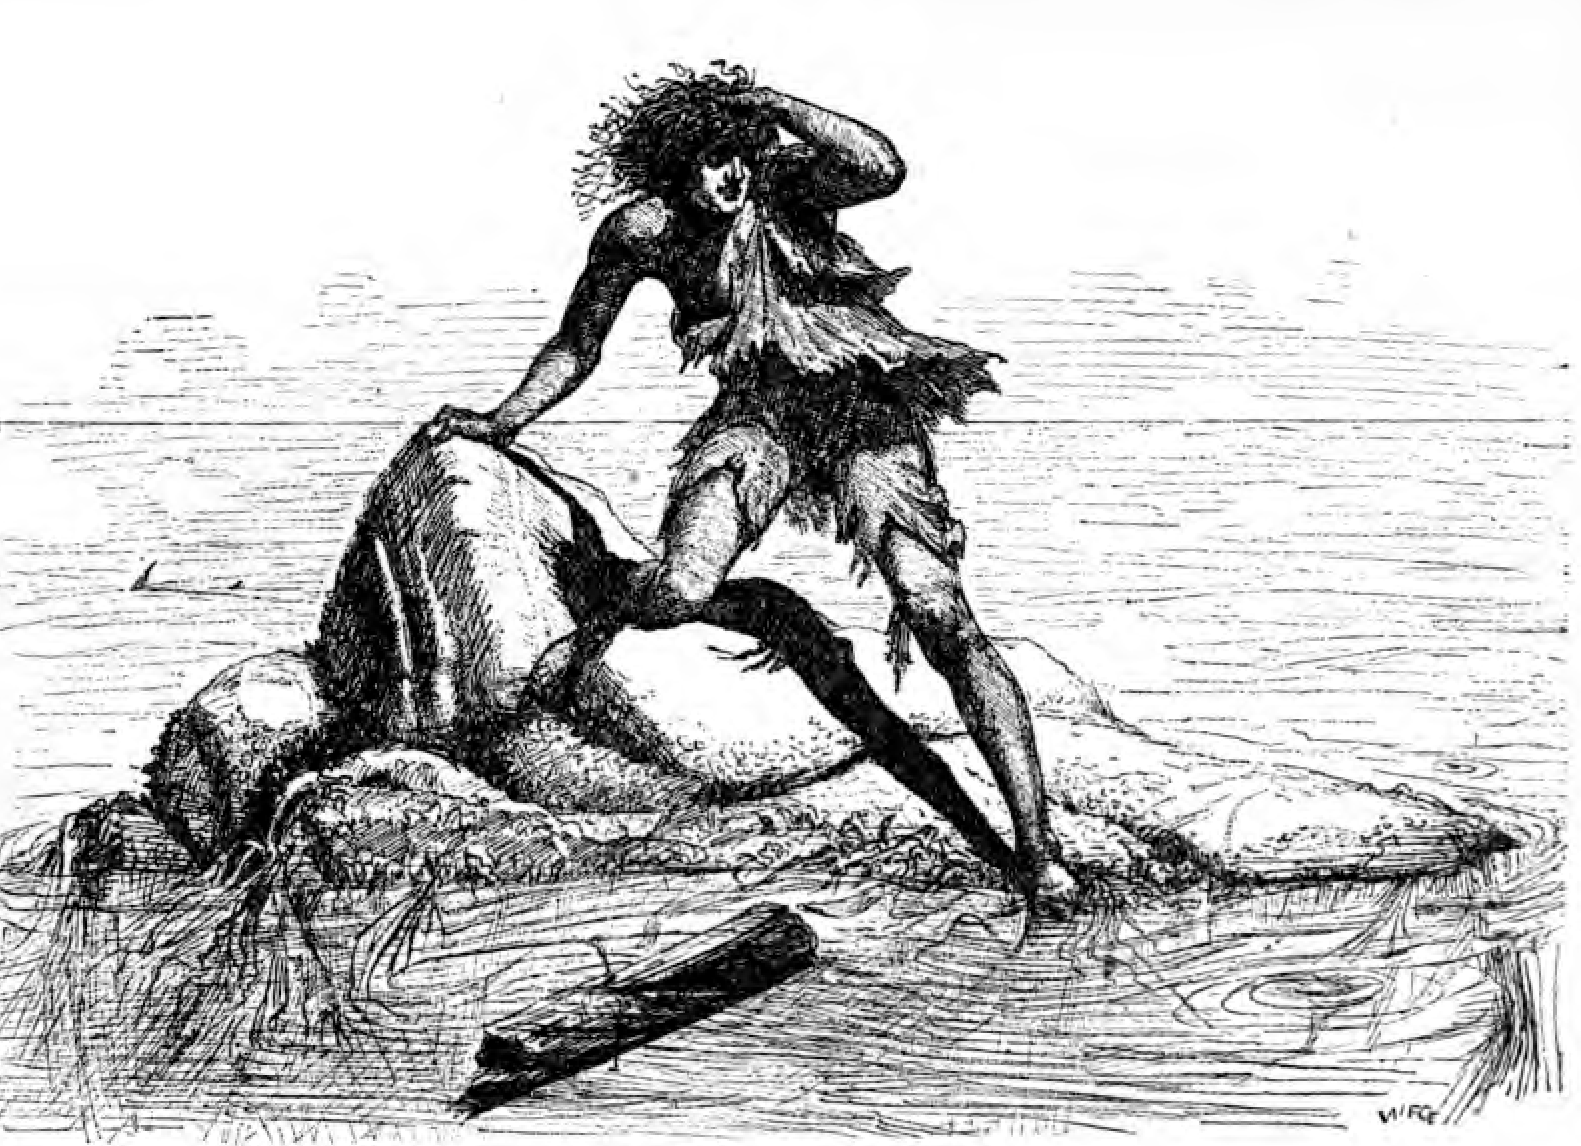
\includegraphics[width=155mm]{./imgs/10.pdf}
\end{figure}

\chapter{Jeltúkhin}

Jeltúkhin\footnote{Jeltúkhin vem de \emph{jóltyi}, ``amarelo'' em russo.}
estava sentado sob o sol numa moita de capim, em um canto entre a
escadaria da entrada e a parede de casa, e olhava com pavor para Nikita, que se
aproximava dele.

A cabeça de Jeltúkhin estava jogada sobre as costas, o bico, com uma
listra amarela por todo o comprimento, postava"-se sobre um papo grosso.
Ele se eriçou e escondeu as perninhas debaixo da barriga. Nikita
curvou"-se em sua direção, e ele abriu a boca para assustar o menino.
Nikita colocou"-o entre as palmas das mãos. Era um estorninho ainda
cinzento --- tinha tentado, pelo visto, voar do ninho, mas as asas
inábeis não o sustentaram e ele caiu, enfiando"-se num canto sobre as
folhas de dente"-de"-leão.

O coração de Jeltúkhin batia desesperadamente: ``Não terei tempo de
dizer um `ah'\,'', pensava o pássaro, ``serei comido imediatamente''. Ele mesmo
sabia como se deve comer minhocas, moscas e lagartas.

O menino o ergueu até a boca. Os olhos pretos de Jeltúkhin cobriram"-se
com uma película, o coração palpitou sob as penas. Mas Nikita somente
soprou em sua cabecinha e o levou para casa: quer dizer que estava
saciado e resolveu comê"-lo mais tarde.

Aleksandra Leóntievna, assim que viu o estorninho, pegou"-o, como Nikita,
na palma da mão e soprou em sua cabecinha.

--- Ainda é tão pequeno, pobrezinho --- disse ela ---, tem o biquinho
amarelo, Jeltúkhin.

Colocaram o estorninho no peitoril de uma janela com vista para o jardim
que tinha sido protegida por uma tela de gaze. Do lado de dentro, a
janela também estava coberta de gaze, mas pela metade. Jeltúkhin no ato
escondeu"-se num canto, querendo mostrar que não entregaria sua vida
facilmente.

Lá fora, atrás da gaze transparente como uma névoa branca, farfalhavam
folhas e brigavam nos arbustos os desprezíveis pardais --- ladrões,
ofensores. Do outro lado, também atrás da gaze, Nikita o fitava com os
olhos grandes, que se moviam, incompreensíveis e encantadores. ``Estou
perdido, estou perdido'', pensou Jeltúkhin.

Mas Nikita até a noite ainda não o tinha comido, somente deixara moscas
e minhocas entre as gazes. ``Querem me engordar'', pensava o pássaro,
fitando de soslaio a minhoca sem olho que se contorcia diante dele
como uma serpente. ``Não vou comê"-la, não é uma minhoca de verdade, é um
engodo.''

O sol se pôs atrás da folhagem. Uma luz cinzenta e sonolenta encobria os
olhos dele, mas Jeltúkhin, com as unhas, agarrava"-se mais fortemente ao
peitoril da janela. Agora seus olhos não viam mais nada. Os pássaros do
jardim se calaram. Espalhava"-se com moleza e doçura cheiro de umidade e
de grama. A cabecinha dele se afundava mais nas penas. Eriçando"-as com
raiva por precaução, Jeltúkhin cambaleou um pouco para a frente, depois
para trás, com a cauda, e dormiu.

Ele foi despertado por pardais, que faziam a algazarra de sempre e
brigavam num galho de lilás. Folhas úmidas pendiam sob uma luz cinzenta.
Ao longe, um estorninho começou a assobiar, produzindo estalidos, doce e
alegre. ``Estou com fome, não tenho mais forças, sinto até enjoo'',
pensou Jeltúkhin e, avistando a minhoca, que se enfiara até a metade
numa frestinha do peitoril, saltou até ela, bicou"-a pela pontinha,
puxou"-a e a engoliu: ``Quem diria, a minhoca era saborosa''.

A luz puxava para o azul. Os pássaros começaram a cantar. E agora um
raio de sol claro e quente caiu através das folhas sobre Jeltúkhin. ``A
vida continua'', pensou ele e, saltando, bicou uma mosca e a engoliu.

Nesse momento, passos ressoaram, Nikita se aproximou e enfiou a mão
enorme por trás da tela; abrindo os dedos, deixou cair moscas e
minhocas no peitoril. Jeltúkhin, horrorizado, enfiou"-se num canto, abriu
as asas e olhou fixamente para a mão; mas ela ficou apenas pendente
sobre sua cabeça e sumiu atrás da tela; então o estorninho voltou a ser
observado por olhos estranhos, fascinantes, irisados.

Quando Nikita foi embora, Jeltúkhin se recompôs e começou a pensar:
``Ele não me comeu, mas poderia. Quer dizer que ele não come pássaros.
Quer dizer que não tenho nada a temer''.

Ele comeu até se fartar, limpou as penas com o bico, ficou saltando ao
longo do peitoril, observando os pardais; elegeu um velho, sem penas no
pescoço, e começou a provocá"-lo, a girar a cabeça, a assobiar: fiuiut,
tchilik"-tchilik, fiuiut. O pardal ficou zangado, inflou as penas e, de
bico aberto, jogou"-se contra Jeltúkhin, batendo na gaze. ``Não me pega,
não me pega'', pensou o estorninho e andou cambaleando pelo peitoril.

Depois Nikita apareceu de novo, enfiou a mão, dessa vez vazia, e levou"-a
para bem perto do pássaro. Jeltúkhin saltou, bicou o dedo dele com
força, pulou para trás e preparou"-se para brigar. Mas o menino
abriu a boca e riu alto: há"-há"-há.

Assim o dia se passou --- não havia nada a temer e a comida era boa, mas
tudo ficou um pouco tedioso. Jeltúkhin mal podia esperar pelo pôr do
sol, e nessa noite dormiu com prazer.

Na manhã seguinte, depois de comer, começou a procurar um jeito de
escapar das telas de gaze. Contornou toda a janela, mas não havia
nenhuma fresta. Então saltou para perto do seu pratinho e bebericou ---
juntava a água no bico, levava a cabeça para trás e engolia, e pela sua
garganta rolava uma bolinha.

Foi um longo dia. Nikita trazia minhocas e limpava o peitoril da janela
com uma pena de ganso. Depois, o pardal careca deu de brigar com uma
gralha, que o bicou de tal jeito que ele caiu como uma pedra nas folhas,
olhando de lá com as penas eriçadas.

Por algum motivo uma pega"-rabuda passou voando bem debaixo da janela,
dava estalidos, agitava"-se, sacudia o rabo, não fazia nada de útil.

Sobre a luz quente do sol, um pintarroxo cantava longa e suavemente
sobre o mel de trevo --- isso fez com que Jeltúkhin entristecesse:
sentiu um fervor na garganta, tinha vontade de cantar, mas onde? Não
nesta janela, não atrás de uma tela!\ldots{}

Jeltúkhin voltou a contornar o peitoril e avistou um animal terrível:
ele estava vindo, andava furtivamente sobre as patas curtas e macias e
arrastava a barriga pelo chão. Sua cabeça era redonda e os bigodes ralos
espetados; os olhos verdes, de pupilas estreitas, brilhavam com uma
raiva diabólica. O estorninho se abaixou e ficou sem se mexer.

O gato Vassíli Vassílievitch saltou suavemente, agarrou com as unhas a
borda do peitoril, olhou através da gaze para Jeltúkhin e abriu a
boca\ldots{} Deus\ldots{} a boca era mais comprida do que o bico dele e tinha
presas\ldots{} O gato bateu com a pata no peitoril, puxou a gaze\ldots{} O coração
de Jeltúkhin paralisou, as asas baixaram\ldots{} Mas nesse momento, bem na
hora, apareceu Nikita, pegou o gato pela pele flácida e o arremessou
porta afora. Vassíli Vassílievitch uivou, magoado, e correu arrastando o
rabo.

``Não há no mundo animal mais forte do que Nikita'', pensou Jeltúkhin
depois desse incidente e, quando o menino se aproximou de novo, o estorninho deixou"-se
acariciar na cabecinha, mas de medo sentou"-se sobre a cauda.

Mais um dia terminou. De manhã, Jeltúkhin, já muito alegre, voltou a
examinar o compartimento, e logo achou o buraco que o gato fizera na
gaze com as unhas. O estorninho enfiou a cabeça ali, olhando para os
lados, atravessou para fora, saltou numa corrente leve de ar e, batendo
rápido, rápido as asinhas, sobrevoou o chão.

Subiu voando junto à porta e avistou quatro pessoas no cômodo vizinho,
todas em volta de uma mesa redonda. Estavam comendo --- pegavam com as
mãos nacos de comida e os enfiavam na boca. As quatro viraram a cabeça
e, sem se mexerem, olharam para Jeltúkhin. Ele entendeu que precisava
ficar no ar e retroceder, mas não conseguiu fazer essa manobra difícil
voando --- caiu sobre uma asa, virou"-se e pousou na mesa entre o vasinho
de geleia e o açucareiro\ldots{} E logo viu Nikita à sua frente. Então, sem
pensar, Jeltúkhin saltou para o vasinho e dali para o ombro do menino,
onde ficou eriçado e semicerrando os olhos cobertos por uma
película.

Depois de um instante no ombro de Nikita, ele voou até o teto, pegou uma
mosca, sentou"-se na figueira do canto, voou ao redor do lustre e,
sentindo fome, foi para sua janela, onde havia minhocas frescas
preparadas especialmente para ele.

Antes de anoitecer, Nikita colocou no peitoril da janela uma casinha de
madeira com um pequeno alpendre, uma portinha e duas janelas. Jeltúkhin
gostou que dentro da casinha estivesse escuro, saltitou para lá, deu uns
giros e dormiu.

Nessa mesma noite, o gato Vassíli Vassílievitch, trancado à chave na
despensa pela tentativa de crime, dava gritos roucos, nem queria mais
caçar ratos; sentado à porta, miava tanto que ele mesmo ficou
aborrecido.

Assim, além do gato e do ouriço, agora na casa passou a viver um
terceiro animalzinho --- Jeltúkhin. Ele era muito independente, sábio e
cheio de vida. Gostava de ouvir as conversas e, quando as pessoas se
sentavam à mesa, ele as escutava, baixando a cabeça, e pronunciava com
voz sonora: ``Sacha'', então se inclinava. Aleksandra Leóntievna tinha
certeza que ele se inclinava para ela. Vendo Jeltúkhin, a
mãezinha sempre dizia: ``Salve, salve, pássaro cinzento, cheio de vida e
de energia''. Ele imediatamente saltava sobre a cauda do vestido de
Sacha e era transportado em cima dela, muito contente.

Assim ele viveu até o outono; cresceu, cobriu"-se de penas negras, como
das asas de um corvo, aprendeu bem a falar russo e, embora passasse
quase o dia todo no jardim, ao entardecer sempre voltava para casa, no
peitoril da janela.

Em agosto ele foi atraído para um bando de estorninhos selvagens que o
ensinaram a voar, e um dia, quando as folhas do jardim começaram a cair,
Jeltúkhin partiu ao clarear com as aves migratórias para o outro lado do
mar, para a África.

\chapter{Klópik}

Os afazeres de primavera no campo terminaram, o pomar foi revolvido e
regado, e agora não havia mais nada para fazer até o dia de São Pedro,
quando a sega começaria. Os cavalos de trabalho foram soltos em manada
para pastar, e eles andavam do outro lado da lagoa, por prados
pitorescos, onde de manhã pairava uma neblina azulada e gigantescos
álamos negros solitários, que pareciam ter crescido do ar nebuloso, pendiam
sobre a terra.

Junto à manada, Michka Koriachónok era o ajudante de tratador. Ele ia
montado numa alta sela cazaque, colocando os pés descalços nos estribos,
tombava para os lados e balançava os cotovelos.

Correndo pelo prado verde atrás de um potro que se separara da manada,
Michka gritava: ``Azát,\footnote{Azát, de origem persa, significa
  ``liberdade''.} volte!'' --- e estalava o chicote, que soava como tiro
de pistola. Depois, ao saltar de seu cavalo desenfreado, que, tilintando
com o bridão, começava a arrancar grama, Michka ora se sentava na borda
de uma vala e raspava um graveto para aplainá"-lo, ora, enrolando as
calças acima dos joelhos, entrava na lagoa e retirava da água morna
bulbos de cebolinhas e raízes de junco, pretas e compridas como
serpentes; as cebolinhas eram azedinhas e crocantes e as raízes
farinhentas e doces. Se comesse em excesso, a barriga começava a doer e
doía muito.

Nikita passava o dia inteiro do outro lado da lagoa na companhia de Michka
Koriachónok e com ele aprendia a montar.

Subir na sela não era difícil: o velho cavalo pardo com pintas marrons
estava calmo, somente batia com a pata traseira no próprio ventre,
afastando mutucas. Mas, quando se acomodava, pegando as rédeas e
deixando"-o trotar, Nikita logo começava a cambalear, ora para o lado
direito, ora para o esquerdo. Quando o cavalo, nem dando trinta passos,
parava e baixava na grama os lábios grossos, Nikita agarrava
convulsivamente a sela e às vezes chegava a rolar pelo pescoço dele,
acabando sob os pés do animal, que reagia a isso com indiferença.
Michka disse:

--- Não fique com medo, cair não dói, somente encolha a cabeça, e que
Deus o livre de agarrar a terra com as mãos --- vá dando cambalhota. Eu
vou mostrar como montar sem sela e sem rédea --- salte e voe.

Michka correu até as éguas de três anos, ainda não domadas, e,
estendendo a mão, começou a chamar a atenção delas:

--- Pão, pão, pão\ldots{}

Até ele correu Estrela, uma égua baia malhada de patas finas, salteadora
de pães, caprichosa, então ergueu as orelhas e, com os lábios
aveludados, procurou por pão. Michka começou a coçar"-lhe o pescoço.
Estrela acenou com a cabeça bem delineada --- gostava daquilo e, para
que Michka também tivesse prazer, começou a pegá"-lo com os dentes pelo
ombro.

Ele acariciou"-a, passando a mão ao longo de seu dorso de cetim (Estrela,
inquieta, trocou as patas de apoio), pegou"-a pela crina e saltou em cima
dela. Surpreendida e zangada, Estrela afastou"-se bruscamente para o
lado, balançou a cabeça, deu um coice, agachou"-se, empinou e saiu
galopando a todo vapor diante da manada.

Michka estava grudado nela feito um carrapato. Então, no meio da
corrida, ela parou e recuou. Ele caiu dando cambalhota e rolou pela
grama. Dirigiu"-se até Nikita mancando, limpando sangue da bochecha
arranhada.

--- Ela me atirou direto nos ramos secos, égua maldita --- disse ele
---, mas você não vai conseguir, está muito gordo.

Nikita ficou calado. Pensou: ``Posso cair de cabeça, mas aprenderei a
montar melhor do que Michka''.

Durante o almoço ele contou sobre Estrela, e a mãezinha ficou
preocupada:

--- Ouça aqui --- disse ela ---, eu imploro que não chegue perto dos
cavalos não domados --- e olhou com uma expressão de súplica para
Vassíli Nikítievitch. --- Vássia,\footnote{Vássia é apelido de Vassíli.}
pelo menos me dê apoio\ldots{} Ele vai acabar quebrando os braços e as
pernas\ldots{}

--- Excelente --- disse em resposta Vassíli Nikítievitch ---, proíba"-o
de andar a cavalo e proíba"-o de andar a pé, também pode quebrar o nariz,
coloque"-o dentro de uma redoma de vidro, embrulhe"-o em tecido e mande"-o
para um museu\ldots{}

--- Eu já sabia --- retrucou mãezinha --- que neste verão eu não teria
um instante de sossego\ldots{}

--- Sacha, o menino já tem dez anos.

--- Ah, isso não faz diferença\ldots{}

--- Perdoe, por favor, mas eu não quero absolutamente que ele vire um
banana infeliz.

--- Sim, mas isso não quer dizer que ele deva ganhar imediatamente
Klópik\footnote{Klópik, em russo, é pequeno percevejo.} de presente.

--- Primeiramente, Klópik pode ser montado até por um bebê.

--- Ele foi ferrado.

--- Não, eu mandei tirar as ferraduras.

--- Ah, neste caso, façam o que quiserem, montem em cavalos bravos,
quebrem as cabeças --- os olhos da mãezinha se encheram de lágrimas, ela
se levantou depressa da mesa e foi para o dormitório.

Vassíli Nikítievitch começou a alisar a barba para os dois lados, jogou o
guardanapo e foi falar com a mãezinha. Arkádi Ivánovitch, que nesse
meio"-tempo fizera de conta que a conversa não tinha que ver com ele,
olhou para Nikita, ajeitou os óculos e disse sussurrando:

--- Sim, irmão, a coisa está feia para o seu lado.

--- Arkádi Ivánovitch, diga à mãezinha que eu não vou cair\ldots{} Palavra,
eu\ldots{}

--- Paciência, controle e firmeza de caráter --- Arkádi Ivánovitch pegou
agilmente uma mosca que teimava em pousar em seu nariz ---, essas três
qualidades são importantes também para se ter habilidade na montaria\ldots{}

Enquanto isso, no dormitório desenrolava uma conversa séria. A voz do
pai ressoava: ``Na idade dele, garotos são totalmente independentes\ldots{}''
``Onde, onde eles são independentes?'', ouvia"-se a voz desesperada da
mãezinha\ldots{} ``Na América eles são independentes\ldots{}'' ``Isso não é
verdade\ldots{}'' ``Mas eu lhe digo que na América um garoto de dez anos é
tão independente quanto eu, por exemplo.'' ``Deus, mas nós não estamos na
América\ldots{}''

As conversas sobre independência continuaram por uma semana inteira. A
mãezinha já entregava os pontos e olhava com tristeza para Nikita, como
se ele estivesse fadado a se machucar, esperando que ao menos a cabeça
fosse poupada.

Durante essa semana, Nikita exercitou montaria aplicadamente do outro
lado da lagoa --- incentivando"-o, Michka mostrou para ele um truque
ousado: saltar sobre o cavalo correndo de trás, como ao brincar de pula
sela.

--- Ele não vai ter tempo de dar coices; e, se der algum, você já estará
no pescoço dele.

Por fim, no café da manhã, na varanda, onde capuchinhas enroladas em
cordas lançavam sombras em movimento sobre a toalha de mesa, os pratos e
os rostos, a mãezinha chamou Nikita, colocou"-o de frente para ela e
disse com voz triste:

--- Você sabe que já tem dez anos e deve ser independente, na sua idade
outros meninos são totalmente, totalmente\ldots{} --- a voz dela tremeu, ela
franziu um pouco o cenho fitando o pai. --- Em suma, o papai tem razão
quando diz que você não é mais criança --- Vassíli Nikítievitch baixou
os olhos, tamborilando na mesa. --- Amanhã nós vamos visitar
Tchembulátova, e você, se quiser, pode ir montando Klópik\ldots{} Eu só peço
que\ldots{}

--- Mãezinha, dou minha palavra, minha palavra de honra, de que comigo
nada acontecerá --- e Nikita beijou a mãezinha, nos olhos, nas
bochechas, no queixo e nas mãos com cheiro de frutas silvestres.

No dia seguinte, depois do almoço antecipado, Vassíli Nikítievitch
mandou Nikita pegar sua sela, a sela de camurça cinza inglesa que lhe
fora dada no Natal. E disse enquanto caminhavam pela grama até a
estrebaria:

--- Você deve aprender a limpar o cavalo, colocar o bridão, a sela,
deixá"-lo descansar depois da cavalgada\ldots{} Quando o cavalo é bem cuidado,
limpo, quer dizer que você é um bom cavaleiro.

Na cocheira bem aberta, atrelaram uma troica à carruagem. O cocheiro,
Serguei Ivánovitch, vestindo um colete e uma camisa cor de framboesa,
mas com um simples quepe na cabeça --- o chapéu com penas ele colocava
somente quando se sentava na boleia ---, endireitava os arreios dos
tirantes no cavalo e xingava Artiom, que o ajudava.

--- Por que você está enfiando a correia debaixo do peito, ignorante!
Estes são os arreios para carruagem. Deixe a correia da coelheira, não
toque nisso. Você devia atrelar um gato num cestinho.

--- É que eu não tenho cavalo.

--- Mas é por ser ignorante que as moças não querem casar com você.
Passe as rédeas novas.

O cavalo do meio da troica, Lorde Byron, amarrado por correias às portas
largas da cocheira, roía o bridão, batia os pés no assoalho de madeira e
tocava de leve no ombro de Serguei Ivánovitch, o qual lhe ajeitava as
franjas que escapavam da rédea. A cocheira cheirava a couro, a suor de
cavalos saudáveis e a pombos. Quando a troica foi atrelada, Serguei
Ivánovitch dirigiu"-se com um sorriso a Nikita:

--- O senhor deseja colocar a sela sozinho?

Klópik foi levado para fora da estribaria. Nikita olhava para ele com
excitação.

Era um cavalo capão ruivo, bem escovado, atarracado, de meias brancas,
rabo espesso, escuro, e crina também escura. Uma grande franja
cobria"-lhe os olhos e através dela ele olhava alegremente abanando
a cabeça. Por suas costas passava uma correia estreita preta.

--- É um bom cavalo --- disse Serguei Ivánovitch, levando"-lhe um balde
de água. Klópik tomou um pouco e levantou a cara, e água escorreu de
seus lábios cinza.

Nikita pegou o bridão e, como lhe ensinaram, introduziu pelo lado o
bocal. Klópik agarrou o ferro com os dentes. Nikita colocou o suadouro,
o xairel cinza com um monograma e por cima de tudo a sela, aí começou
a apertar as barrigueiras --- a coisa não era brincadeira.

--- Está inflando a barriga --- disse Serguei Ivánovitch ---, é um
animal esperto --- e ele deu um tapa na barriga de Klópik; o capão
soltou o ar e Nikita apertou as barrigueiras.

Vassíli Nikítievitch aproximou"-se e começou a dar ordens:

--- Pegue a rédea na mão esquerda, aproxime"-se pela frente do cavalo,
pelo lado esquerdo. Monte. Aperte"-o com as batatas das pernas. Não tire
os pés dos estribos, não dobre as pontas dos pés.

Nikita montou, achando com o pé trêmulo o estribo direito que lhe
escapava, tocou no cavalo com os pés, e Klópik começou a trotar em
direção à estrebaria.

Vassíli Nikítievitch gritou:

--- Pare! Pare! Use a rédea direita, cabeça de vento!\ldots{}

Na estrebaria, na sombra, Klópik parou. Nikita, morrendo de vergonha,
saltou, pegou o cavalo pela rédea e o levou para a saída, sussurrando
para o esperto animal:

--- Você é um porco, um porco de verdade, um tolo infeliz!\ldots{}

Klópik acenava alegremente com a franja. Serguei Ivánovitch disse ao se
aproximar:

--- Monte, eu vou conduzir daqui. É um capão muito esperto. Ele não quer
trabalhar, quer ficar na sombra.

Finalmente Klópik foi dominado, e Nikita cavalgou a trote lento em
frente aos currais.

Serguei Ivánovitch colocou o chapéu com penas e as luvas polvilhadas de
farinha, sentou"-se na boleia e gritou severamente:

--- Soltem!

Artiom, que segurava Lorde Byron pelo bridão, saltou para o lado, e a
troica, arrancando e batendo nas tábuas do assoalho, saiu velozmente da
cocheira, brilhando com o verniz e o cobre da carruagem e lançando
torrões de lama fresca pelos cascos dos cavalos laterais, e a parelha,
repicando os guizos, fez um semicírculo pelo quintal verde e parou na
frente de casa.

Aleksandra Leóntievna, com um vestido branco, desceu pela escadaria da
entrada e, abrindo uma sombrinha branca, olhou alarmada para Nikita, que
montava ao longe. O pai ajudou a acomodar a mãezinha na carruagem,
depois saltou ele mesmo para dentro.

--- Vamos!

Serguei Ivánovitch ergueu as rédeas. Os magníficos animais baios,
pedindo para serem soltos dos duros bridões, conduziam a carruagem com
leveza e atravessaram com estrondo a pontezinha. Os cavalos laterais
começaram a galopar mexendo os quadris. Lorde Byron, sentindo que aquilo
não passava de brincadeira, mexia as orelhas. A mãezinha olhava para
trás a cada minuto. Nikita, curvando"-se, afrouxou as rédeas e
rapidamente alcançou a troica.

Ele queria correr desabaladamente, mas Klópik decidiu que isso não era
necessário, e, quando emparelhou com a carruagem, voltou para a estrada
e começou a trotar bem atrás das rodas, numa nuvem de poeira. Nenhuma
força poderia detê"-lo ou desviá"-lo de seu caminho: tudo isso ele
considerava supérfluo --- para ele andar significava andar pela
estrada, e não discutiria à toa.

A mãezinha continuava se virando para trás. Nikita sacudia"-se, apertando
a boca, olhando tensamente entre as orelhas do cavalo. Sentia náuseas
com a poeira e o trote de Klópik lhe revirou o estômago.

--- Quer passar para a carruagem?

Nikita meneou a cabeça negativamente. O pai, rindo, disse a Serguei
Ivánovitch:

--- Aperte o passo!

Lorde Byron levantou as orelhas e disparou jogando os pés de ferro para
a frente, e os cavalos laterais o seguiram pela relva. Klópik passou
para o galope, mas a carruagem se afastava, e ele, ficando zangado,
agora galopava com todas as forças, se empenhando terrivelmente.

O sentimento desagradável do trote regular havia passado. Nikita estava
montado em sua sela, gracioso e firme, o vento assobiava nos ouvidos,
dos dois lados da estrada passavam ondas de cereais verdes, e cotovias,
invisíveis à luz do dia, cantavam com vozes simplesinhas. Era quase tão
bom como ler Fenimore Cooper.

A carruagem começou a andar a passos lentos. Nikita alcançou"-a e,
resfolegando, olhou alegremente para o pai.

--- Tudo bem, Nikita?

--- Tudo maravilhoso\ldots{} Klópik é um cavalo fora de série\ldots{}


\begin{figure}
\vspace*{-2.65cm}
\hspace*{-2.85cm}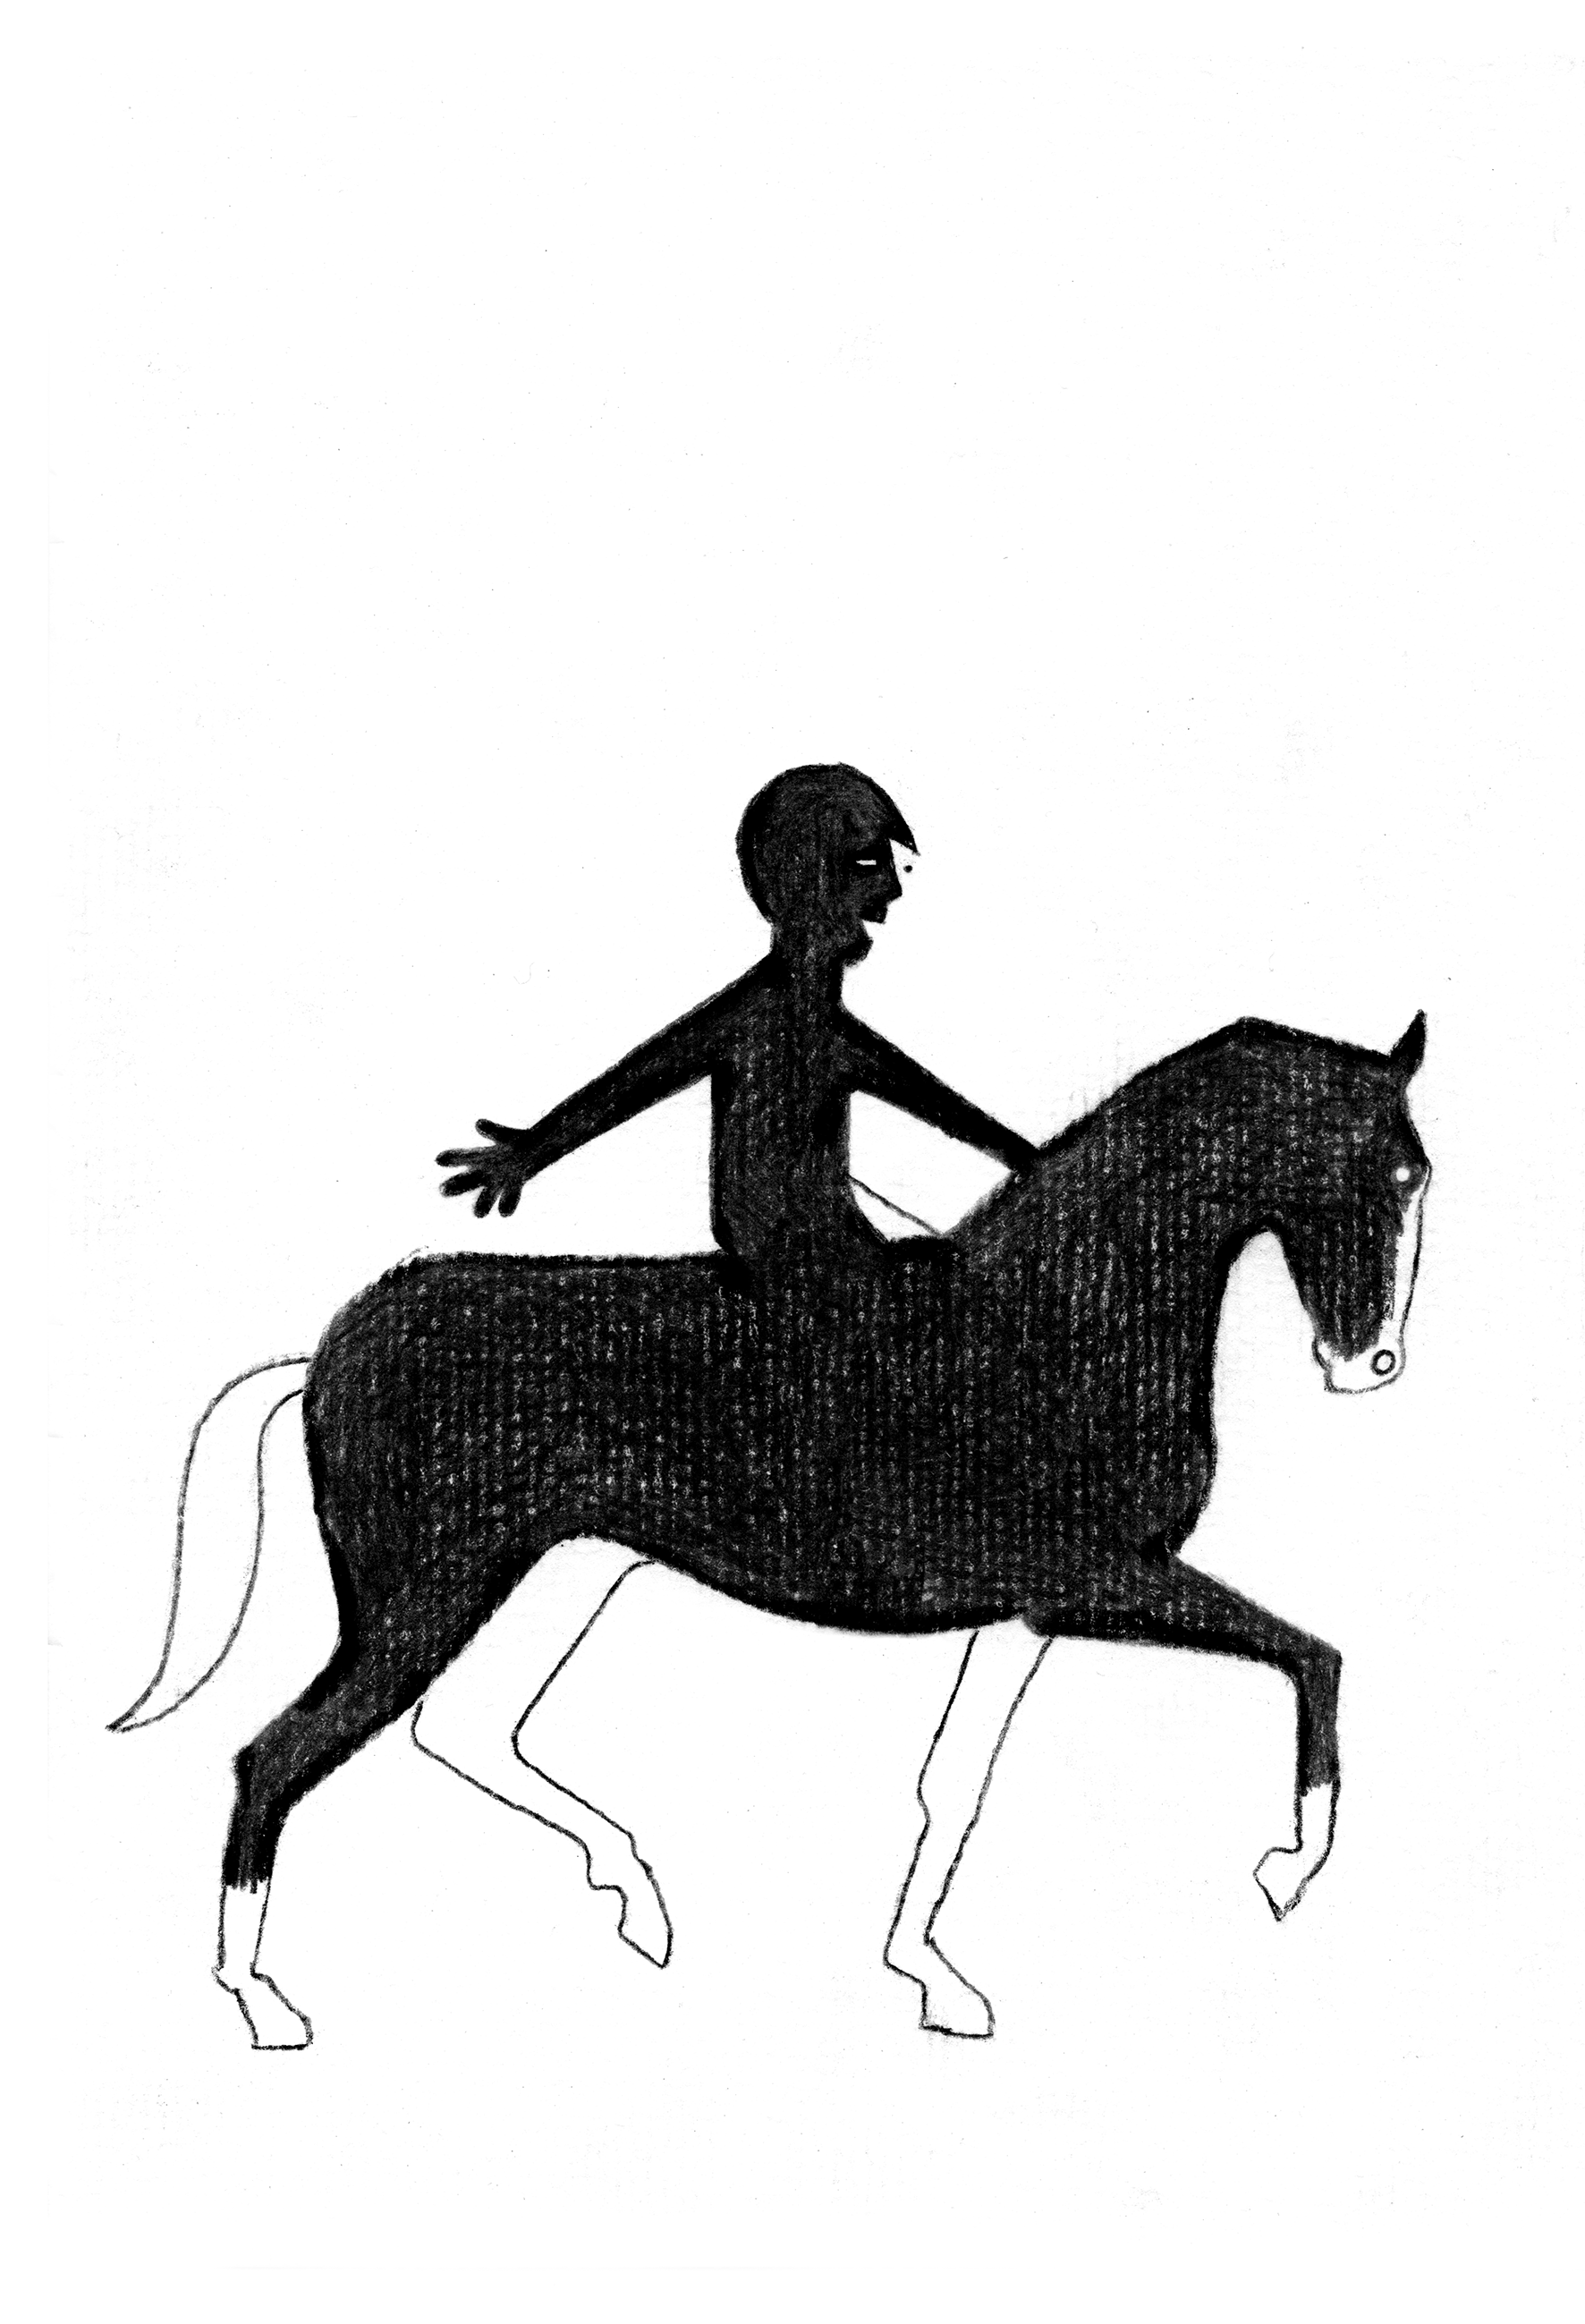
\includegraphics[width=155mm]{./imgs/11.pdf}
\end{figure}


\chapter{No balneário}

Numa manhã cedo, Vassíli Nikítievitch, Arkádi Ivánovitch e Nikita
caminhavam em fila para a lagoa através de uma trilha de grama acinzentada pelo
orvalho; estavam indo se banhar.

A névoa da manhã ainda podia ser vista nas partes densas do jardim. Numa
clareira, sobre vassouras amarelas com mel e trevos brancos, borboletas
empurravam"-se como folhas leves e uma abelha voava, preocupada. Na mata,
um pombo selvagem arrulhava fechando os olhos, inflando o peitinho;
arrulhava com tristeza e doçura, dizendo que tudo será como sempre foi,
tudo passará e voltará a ser como era.

Vassíli Nikítievitch, para chegar ao balneário de tábuas, transpôs as passarelas compridas de madeira que estalavam ao bater na água, aí,
sentado num banco à sombra, tirou a roupa dando palmadas no peito peludo
e branco e nos flancos lisos, entrefechando os olhos por causa do reflexo
ofuscante da água e dizendo:

--- Ótimo, excelente!

Seu rosto bronzeado, de barba lustrosa, parecia ter sido acoplado a um
corpo branco. Do pai emanava um cheiro de saúde particularmente
agradável. Quando uma mosca pousava em sua perna ou no seu ombro, ele
dava um tapa sonoro com a palma da mão, deixando em seu corpo uma mancha
rosada. Depois de se refrescar, o pai pegava um sabonete perfumado, tão
leve que não afundava na água, descia cuidadosamente para o balneário
por uma escadinha escorregadia devido ao musgo verde --- a água
ficava"-lhe na altura do peito --- e começava a ensaboar a cabeça e a
barba com força, bufando e repetindo:

--- Ótimo, excelente.

Por cima do balneário, uma nuvem de mosquitos pairava à luz azulada do
sol. Entrou voando uma libélula, trepidando, olhou com olhos
esbugalhados de esmeralda para a cabeça ensaboada de Vassíli
Nikítievitch e voou de lado. Arkádi Ivánovitch, enquanto isso, tirou
rápida e acanhadamente a roupa, apertando os dedos compridos dos pés um
pouco tortos, então abriu a porta de fora do balneário, olhou para os
lados --- para ver se não havia ninguém espiando na beirada ---, disse com
voz de baixo: ``Ótimo'', e se jogou de barriga na lagoa. A água espirrou
com estrondo, as gralhas, assustadas, subiram nos galhos, e ele mesmo
nadava de braçada, com o corpo magro de pelos ruivos, serpenteando sob a
água azulada.

Chegando a nado até o meio da lagoa, Arkádi Ivánovitch dava cambalhotas,
mergulhava e gritava como um monstro aquático: ``Uh"-brrrr\ldots{}''.

Nikita estava sentado num banco resinoso, com as pernas encolhidas
contra o peito, e esperava o pai terminar de se ensaboar. Vassíli
Nikítievitch colocou o sabonete e a esponja na escadinha, tapou os
ouvidos e mergulhou três vezes --- seus cabelos molhados grudaram, a
barba ficou pendente, parecendo uma cunha, e toda a sua aparência
tornou"-se abominável, eles até deram um nome para isso: ``criando o
abominável Vássia''.

--- Então, vamos nadar --- disse subindo para a passarela de fora,
jogou"-se pesadamente na lagoa e nadou como uma rã, rapidamente,
impulsionando"-se com mãos e pernas na água translúcida.

Nikita voou para dentro da lagoa, deu uma cambalhota e, alcançando o
pai, passou a nadar ao lado dele, esperando um elogio: nesse verão
aprendera a nadar com destreza ao brincar com os garotos no rio Tchagrá
--- sabia nadar de lado, de costas, ficar em pé e girar debaixo d'água.
O pai propôs, sussurrando:

--- Vamos afundar o Arkádi.

Eles se separaram e nadaram por dois lados na direção de Arkádi
Ivánovitch, que, por causa da miopia, não notava o cerco. Ao chegarem
perto, nadando de braçada, jogaram"-se contra ele. Arkádi Ivánovitch
urrou de raiva, começou a se debater, expondo"-se até a
cintura, e mergulhou. Foi pego pelos pés --- o que mais temia neste
mundo eram cócegas. Mas agarrá"-lo não era fácil, ele escapava a todo
momento. Quando Vassíli Nikítievitch e Nikita voltaram para o
balneário, Arkádi Ivánovitch já estava lá sentado num banco, de roupa de
baixo e óculos, e disse com uma risada irônica:

--- Os senhores precisam aprender a nadar.

Voltando da lagoa, eles geralmente encontravam Aleksandra Leóntievna com
uma touquinha branca e um penhoar felpudo. A mãezinha, semicerrando os
olhos contra o sol, dizia sorrindo:

--- O chá está posto no jardim, debaixo da tília. Sentem, não me esperem
--- os pãezinhos vão esfriar.

\chapter{A agulha do barômetro}

Já fazia alguns dias que Vassíli Nikítievitch batia com as unhas no
barômetro e praguejava baixinho diante da agulha em pé: ``seco, muito
seco''. Em duas semanas não caíra uma gota de chuva, e era época de
amadurecimento dos cereais. A terra rachava, o calor empalideceu o céu
e, ao longe, acima do horizonte, pairava uma bruma escura lembrando a
poeira de uma manada. Os prados queimaram, desbotaram, as folhas das
árvores começaram a se enrolar, e, por mais que Vassíli Nikítievitch
batesse no vidro do barômetro, a agulha teimosamente mostrava: ``seco,
muito seco''.

Juntando"-se ao redor da mesa, as pessoas de casa não brincavam como
antes --- os rostos do pai e da mãe estavam preocupados; Arkádi
Ivánovitch também ficava quieto, olhava para dentro do prato e, de
tempos em tempos, ajeitava os óculos, tentando disfarçar um suspiro
contido. Mas ele tinha seus motivos: Vassa Nílovna, a professora da
cidade que prometera passar um tempo em Sosnovka, escrevera que ``estava
presa à cama da mãe adoentada'' e esperava encontrar"-se com Arkádi
Ivánovitch somente no outono, em Samara.

Nikita assim imaginava Vassa Nílovna: uma mulher alta e desanimada, de
blusinha cinza, um relógio com um cordão, e uma perna presa com corrente
ao pé de uma cama. Nesses dias sufocantes e opacos, por causa de uma
névoa seca, a imagem de uma professora sentada junto a uma parede nua,
perto de uma cama de ferro, era especialmente triste.

No almoço, Vassíli Nikítievitch, tamborilando uma polca na beirada do
prato, disse:

--- Se amanhã não chover, a safra estará perdida.

A mãezinha imediatamente abaixou a cabeça. Como em um delírio, ouviam
uma mosca ressoar na enorme janela, na parte de cima, onde havia vidros
duplos semiarredondados que, por nunca serem limpos, cobriam"-se de teias
de aranha. A porta de vidro que dava para a varanda estava fechada, para
que o calor do jardim não fosse levado para dentro.

--- Será que teremos mais um ano de fome? --- perguntou a mãezinha. ---
Deus, como é terrível!

--- Pois é: fique sentado e espere pela sentença --- o pai aproximou"-se
da janela e olhou para o céu, enfiando as mãos nos bolsos das calças de
seda ---, mais um dia deste calor infernal, e teremos um inverno
faminto, tifo, extinção de gado, óbito de crianças\ldots{} Isso é
inconcebível.

O almoço terminou em silêncio. O pai foi dormir. A mãezinha foi chamada
à cozinha para contar a roupa de baixo. Arkádi Ivánovitch, que sentia uma
tristeza imensa por dentro, saiu sozinho para passear na estepe
escaldante.

Nos quartos, no silêncio lúgubre do meio"-dia, somente moscas zuniam,
todas as coisas estavam como que cobertas de poeira. Nikita não sabia
onde se esconder. Foi até a escadaria da entrada. Sob o sol nebuloso mas
com uma luz branca especialmente ofuscante, o amplo quintal estava
deserto e silencioso --- tudo adormeceu, ficou imóvel. A cabeça zunia de
silêncio e de calor.

Nikita foi para o jardim, mas lá também não havia vida. Uma abelha
passou zunindo. Inertes, as folhas empoeiradas pendiam como se fossem de
lata. O barco estava cravado na água opaca da lagoa, e gralhas o
mancharam de branco.

Nikita foi para casa e se deitou em um pequeno sofá com cheiro de rato.
No meio da sala, a mesa de jantar postava"-se descoberta sobre uma
infinidade de pezinhos detestáveis. Não havia neste mundo nada mais
tedioso do que aquela mesa. Ao longe, na cozinha, a cozinheira cantava
em voz baixa --- talvez estivesse limpando as facas com tijolo moído ---,
entoava lamentos, a meia voz, de uma tristeza mortal.

Eis que, numa janela entreaberta, Jeltúkhin apareceu, no peitoril, com o
bico aberto de calor. Tomando ar, sobrevoou a mesa e pousou no ombro de
Nikita. Virou a cabecinha, fitou"-o nos olhos e bicou"-o na têmpora,
bem onde o menino tinha um sinal de nascença que lembrava um grãozinho
--- então o pássaro o beliscou e de novo o fitou nos olhos.

--- Deixe"-me, por favor, vá embora --- disse Nikita e se levantou
preguiçosamente, vertendo um pouco de água num pires para o estorninho.

Jeltúkhin bebericou, saltou no pires, banhou"-se, derramou toda a água, alegrou"-se e, voando à procura de um lugar para sacudir"-se, pousou na cornija do estojo de madeira do barômetro.

--- Fiuit --- disse Jeltúkhin com voz suave ---, fiuit, tempeeestade.

--- O que está dizendo? --- perguntou Nikita e aproximou"-se do
barômetro.

Jeltúkhin, sentado na cornija, inclinou"-se e baixou as asas. Balbuciava
algo na língua dos pássaros e na língua russa. E, nesse momento, Nikita
viu que a agulha azul do mostrador afastou"-se muito da agulha dourada,
oscilando entre ``instável'' e ``tempestade''.

Nikita tamborilou no vidro e a seta deslocou"-se mais para
``tempestade''. Ele correu para a biblioteca, onde o pai estava
dormindo. Bateu na porta. Uma voz sonolenta e confusa respondeu
rapidamente:

--- Que é? Que foi?

--- Papai, vá olhar o barômetro\ldots{}

--- Não importune, Nikita, eu estou dormindo.

--- Papai, vá ver o que está acontecendo com o barômetro\ldots{}

Na biblioteca estava silencioso e o pai, pelo visto, não conseguia
acordar. Finalmente, ouviram"-se batidas de pés descalços, a chave virou
e, pela porta entreaberta, enfiou"-se uma barba desgrenhada:

--- Por que me acordou?\ldots{} O que aconteceu?

--- O barômetro está mostrando ``tempestade''.

--- Está mentindo --- o pai disse sussurrando, assustado, correu até
a sala e no mesmo instante gritou de lá para toda a casa: ---
Sacha, Sacha, tempestade!\ldots{} Hurra!\ldots{} Estamos salvos!

A angústia e o calor aumentavam. Os pássaros se calaram, as moscas
ficaram sonolentas nas janelas. Perto de escurecer, o sol, já baixo,
desapareceu numa névoa incandescente. O pôr do sol chegou rapidamente.
Estava completamente escuro --- nem uma estrela no céu. A agulha do
barômetro mostrava firmemente ``tempestade''. Todos se reuniram e
sentaram"-se ao redor da mesa redonda de quarenta pezinhos. Falavam em
sussurros, lançavam olhares às portas escancaradas da varanda que davam
para o jardim invisível.

Eis que, no silêncio mortal, os salgueiros da lagoa ressoaram um som
abafado e imponente, então chegaram os gritos assustados das gralhas. O
pai saiu para a varanda na escuridão. Os ruídos se tornavam mais
intensos, mais solenes, e finalmente uma forte rajada de vento entortou
a acácia perto da varanda, um odor agradável infundiu"-se da porta,
folhas secas entraram, a luz no globo opaco da lâmpada piscou, e o vento
começou a zunir, a uivar nas chaminés e nos cantos da casa. Uma janela
bateu em algum lugar, e vidros quebrados tilintaram. Agora, todo o
jardim estava ruidoso, os troncos rangiam e suas copas invisíveis
balançavam. Vindo da varanda, Vassíli Nikítievitch surgiu despenteado,
boquiaberto, os olhos dilatados. E então, sob uma luz ofuscante
branco"-azulada, a noite despontou, por um instante apareceram as
silhuetas de árvores pendendo para baixo. E de novo a escuridão. Veio um
estrondo, e o céu desmoronou. Por causa do barulho, ninguém notou quando
começaram a jorrar gotas de chuva nas vidraças. Desabou a chuva ---
forte, abundante, torrencial. A mãezinha se postou na porta da varanda
com os olhos cheios de lágrimas. O cheiro de umidade, bolor,
chuva e grama encheu a sala.

\begin{figure}
\vspace*{-2.65cm}
\hspace*{-3.25cm}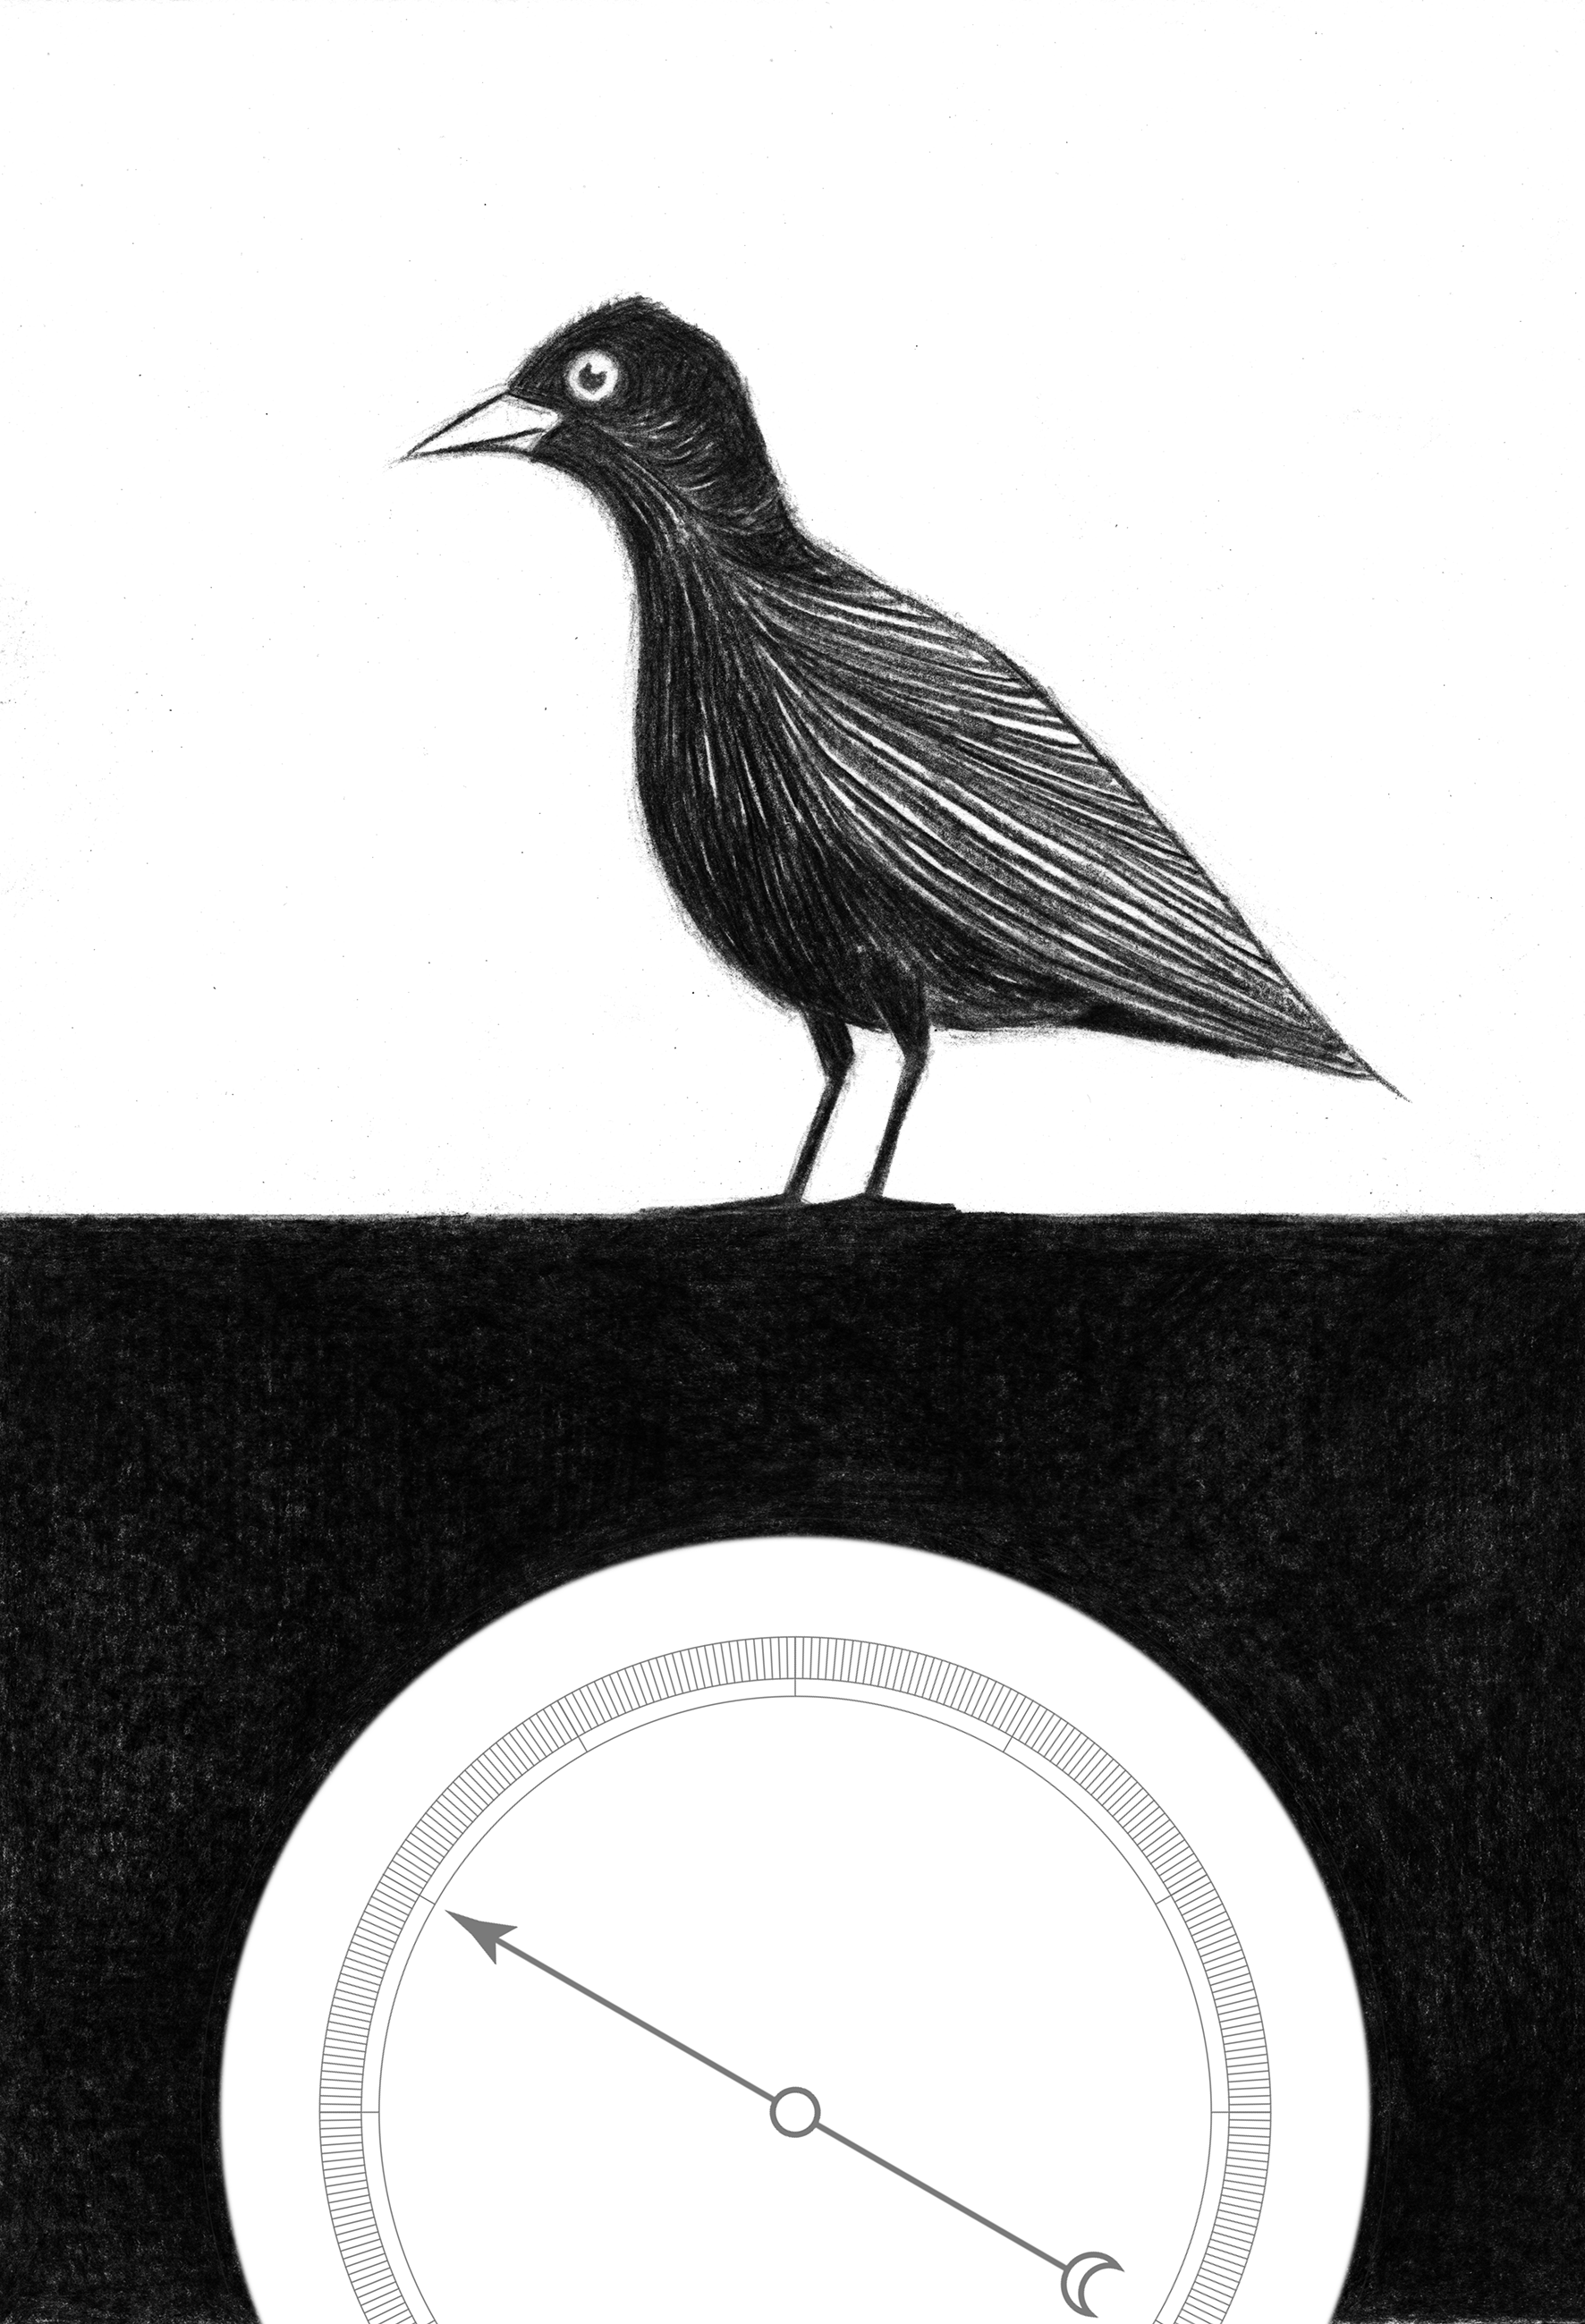
\includegraphics[width=155mm]{./imgs/12.pdf}
\end{figure}

\chapter{A cartinha}

Nikita saltou da sela, amarrou Klópik num prego de um poste listrado e
entrou no posto de correios, que ficava na praça da feira da vila
Utievka.

Atrás de uma cerca aberta, estava sentado o chefe dos correios,
desgrenhado, de rosto inchado, queimando lacre com uma vela. Sua mesa
estava toda suja de pingos de lacre e de tinta, coberta de cinzas de
tabaco. Ao pingar uma porção de lacre quente no envelope, ele pegou com
a mão peluda um carimbo e com ele bateu de tal jeito na carta que
parecia querer quebrar o crânio do remetente. Depois, tirou da gaveta um
selo, botou a língua grande para fora, lambeu"-o, colou"-o, cuspiu com
nojo, e só então olhou enviesado, com os olhos inchados, para Nikita.

O chefe dos correios atendia pelo nome de Ivan Ivánovitch Lándychev. Ele
tinha costume de ler todos os jornais e revistas: lia"-os de cabo a rabo
e, enquanto não terminasse, não os entregava de jeito nenhum. Inúmeras
vezes se queixaram dele em Samara, porém ele só ficava mais zangado e
não parava com a leitura. Seis vezes por ano entregava"-se à bebedeira,
e nessas ocasiões tinham medo até de pisar no posto. O chefe dos
correios aparecia na janelinha e gritava para toda a praça: ``Engoliram
a minha alma, canalhas!''.

--- O papai me mandou pegar a correspondência --- disse Nikita.

O chefe dos correios não respondeu nada е voltou a acender o lacre, que
pingou na sua mão, então o homem saltou, deu um gritou e sentou"-se de
novo.

--- Por que eu deveria saber quem é seu papai? --- disse com extrema
hostilidade. --- Cada um aqui é um papai, aqui todos são papais\ldots{}

--- O que o senhor está dizendo?

--- Que vocês têm milhares de papais, é isso que estou dizendo --- o
chefe dos correios até cuspiu debaixo da mesa. --- Sobrenome, sobrenome,
preciso saber qual é o sobrenome do seu papai --- ele largou o lacre
e, depois da resposta de Nikita, tirou da gaveta um maço de cartas.

Nikita colocou"-as na bolsa e perguntou timidamente:

--- Será que não há revistas, jornais?

O chefe dos correios começou a bufar. Nikita, sem esperar uma resposta,
desapareceu atrás da porta.

Klópik, que estava junto ao poste dos correios, batia com a pata no chão
e se chicoteava com o rabo para espantar as moscas. Dois garotos, com
rostos sujos de borra de \emph{kvás}\footnote{\emph{Kvás}, bebida russa feita à
  base de pão fermentado de centeio.} e cabelos sedosos, olhavam para o
cavalo.

--- Saiam daqui --- gritou Nikita e sentou"-se na sela.

Um dos garotos sentou no chão empoeirado, o outro se virou e correu.
Através da janela se via de novo o lacre na mão do chefe dos correios.

Saindo da vila e chegando à estepe quente, tingida de amarelo"-ouro pelos
cereais maduros, Nikita deixou Klópik andar livremente e abriu a bolsa
para examinar a correspondência.

Uma das cartas era pequena, em um envelopinho lilás assinalado com
letras grandes --- ``Entregar para Nikita''. A cartinha tinha sido
escrita em papel rendado. Piscando de emoção, ele leu:

``Querido Nikita, eu não me esqueci de você. Eu amo muito você. Nós
estamos morando na \emph{datcha}.\footnote{\emph{Datcha}, casa de veraneio russa.} E a nossa \emph{datcha} é muito boa.
Mesmo que Víktor me importune e não me deixe viver. Ele não obedece mais
a mamãe. Pela terceira vez cortaram os cabelos dele com a maquininha e
ele está sempre todo arranhado. Eu passeio sozinha pelo nosso jardim.
Nós temos um balanço e até maçãs, mas elas ainda não amadureceram. Ainda
se lembra do bosque encantado? Venha nos visitar em Samara no outono.
Ainda não perdi seu anelzinho. Adeus, Lília''.

Nikita leu essa carta surpreendente repetidas vezes. Ela trouxe de volta
o encanto dos dias do Natal passado. Velas se acenderam. Uma sombra
tremulando na parede, um grande laço sobre os olhos azuis e
muito atentos da menina, correntes de papel farfalhando na árvore
de Natal, a luz da lua brilhando nas janelas cobertas de gelo. Uma luz
irreal inundou os telhados cheios de neve, as árvores brancas, os campos
nevados\ldots{} Debaixo da lâmpada, junto à mesa redonda, de novo estava
sentada Lília, apoiada em seu punho\ldots{} Pura magia!\ldots{}

Nikita soergueu"-se nos estribos, levantou o chicote e pegou desprevenido
Klópik, que se jogou para o lado e começou a galopar. O vento assobiava
nos ouvidos sem cessar. Uma águia plainava bem no alto sobre a ampla
estepe, sobre os cereais maduros, em alguns lugares já ceifados, e sobre
o penhasco de barro do rio. Num vale perto de um lago salgado, abibes
solitários gritavam lamentos. ``Corra, corra, corra!'', pensava Nikita.
Seu coração estava alegre e batia acelerado. ``Assobie, assobie,
vento!\ldots{} Voe, voe, pássaro águia!\ldots{} Grite, grite, abibe --- eu sou
mais feliz do que você. O vento e eu, o vento e eu\ldots{}''

\begin{figure}
\vspace*{-2.65cm}
\hspace*{-2.85cm}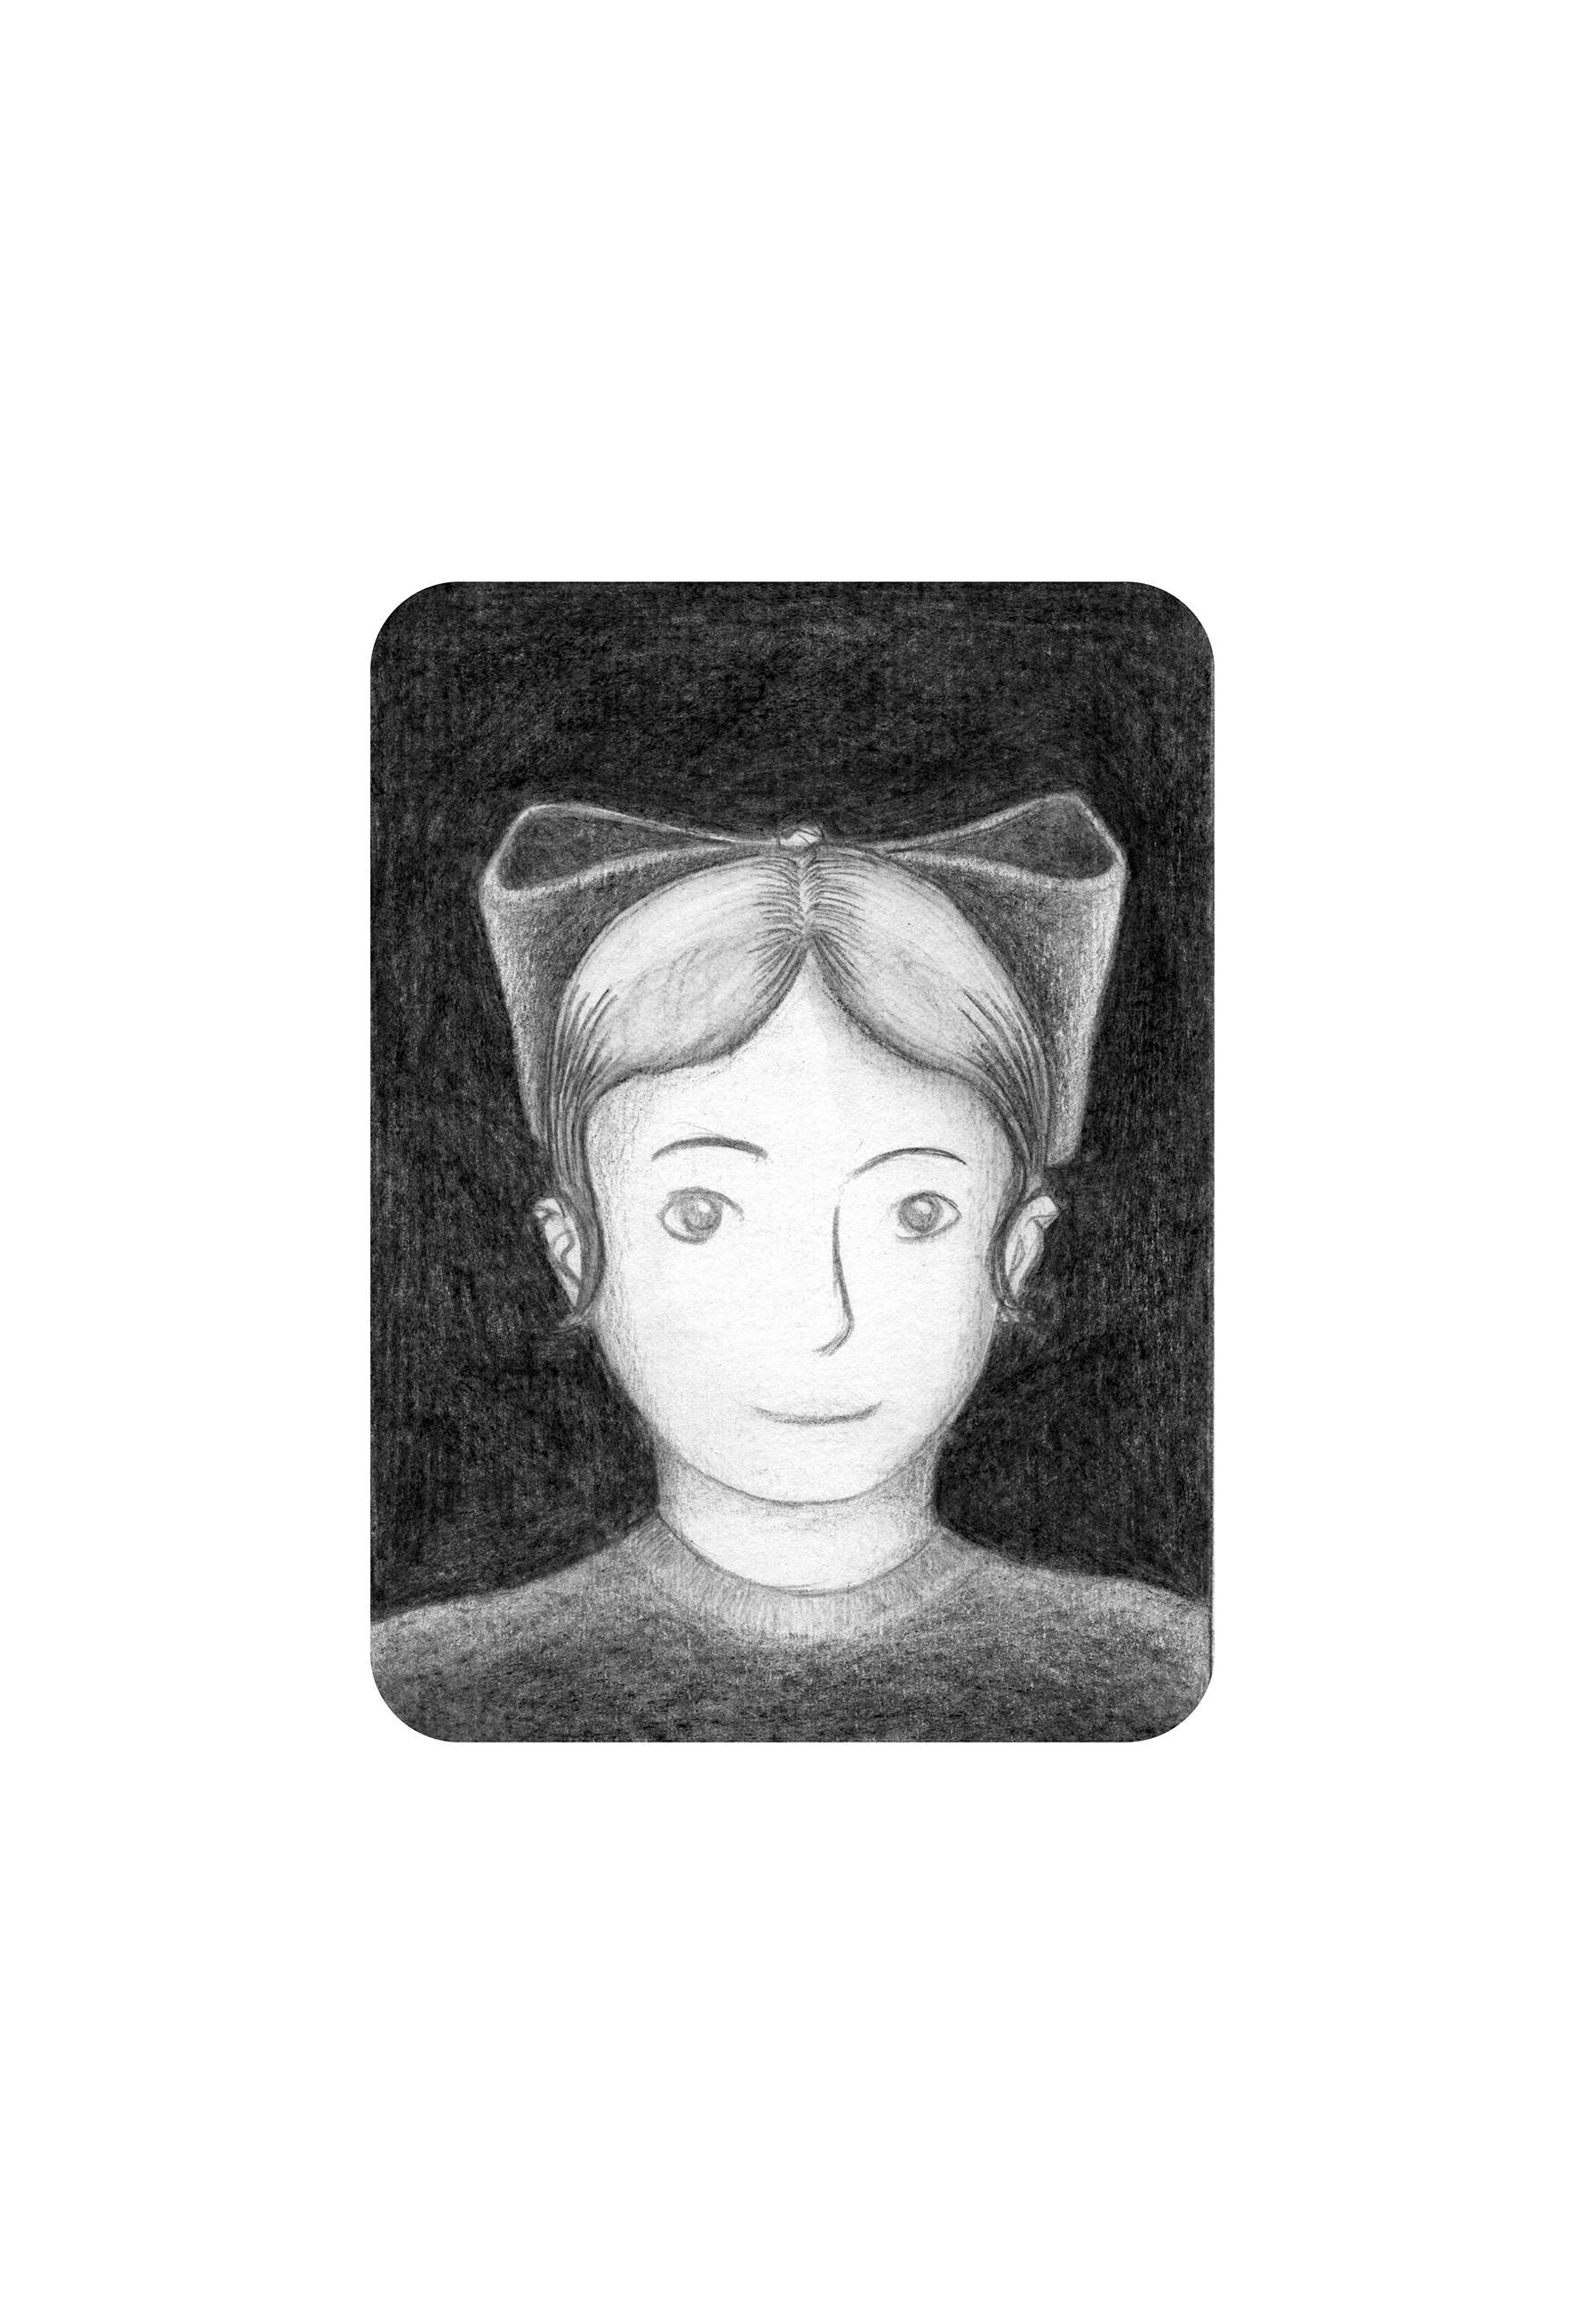
\includegraphics[width=155mm]{./imgs/7.pdf}
\end{figure}

\chapter{A feira em Pestravka}

Era o terceiro dia que Vassíli Nikítievitch e a mãezinha estavam
brigando: o pai queria muito viajar à feira em Pestravka, já a mãezinha
estava decididamente contra a viagem:

--- Em Pestravka, meu amigo, vão se arranjar maravilhosamente sem você.

--- Estranho --- respondeu o pai, pegando um punhado da barba,
mordendo"-a e encolhendo os ombros ---, isso é muito estranho.

--- Então que seja estranho, meu amigo.

--- Não, isso é estranho em alto grau!

--- Eu insisto --- dizia a mãezinha ---, nós não precisamos de novos
cavalos: graças a Deus, temos cavalos de sobra, a estrebaria está cheia.

--- Entenda de uma vez que estou viajando para vender a maldita égua
Zaremka.

--- É pena, Zaremka é uma égua maravilhosa.

--- O que você está dizendo?! --- perguntou o pai, afastando as pernas e
esbugalhando os olhos. --- Zaremka morde e dá coice.

--- Não --- disse a mãezinha, decidida ---, Zaremka não morde nem dá
coice.

--- Neste caso --- o pai até fez uma reverência ---, dou um ultimato: ou
essa maldita égua deixa esta casa, ou a deixo eu!

No fim das contas, a mãezinha, como Nikita havia imaginado, preferiu o
pai. A disputa terminou com trégua e concessões: foi decidido vender a
égua, mas o pai deu a palavra de ``não gastar um dinheiro absurdo na
feira''.

Para poupar, Vassíli Nikítievitch inventou de mandar para
Pestravka duas carroças de carga com maçãs --- caídas das árvores --- e
vendê"-las a granel.

Nikita pediu permissão para viajar nas carroças com Michka Koriachónok.

Desde a manhã começaram os obstáculos. Os cavalos não estavam
preparados, e Michka Koriachónok, montando num cavalo lateral da troica,
foi até a manada, que estava pouco visível na névoa esfumaçada da manhã
que se acumulara nos declives atrás das lagoas. Depois, quando trouxeram
da estrebaria Zaremka, ruiva e de meias brancas, e começaram a escová"-la
com a almofaça, a égua pegou Serguei Ivánovitch com os dentes e por
pouco não o matou. O pai viu isso da janela e, ainda de roupa de baixo,
correu até a estrebaria.

--- A"-há, ela morde!\ldots{} O que foi que eu lhes disse, diabos?!\ldots{}

Zaremka começou a andar para trás, agachou"-se, arrastou Serguei
Ivánovitch pelo cabresto, relinchou, desgarrou e, baixando a cabeça e
dando coices que fizeram os torrões de lama de seus cascos voarem acima
da cocheira, saiu galopando para a manada. Depois, desapareceu Artiom,
que deveria ir com as carroças. Foram procurá"-lo e revelou"-se que, desde
a véspera, estava preso em uma cela de uma isbá do distrito: chegara o
tempo de pagar os tributos e já fazia pelo menos cinco anos que Artiom
não os pagava. Em qualquer lugar que o encontrassem, os chefes deveriam
apanhá"-lo e colocá"-lo numa cela, até que alguém o resgatasse, pagando
por ele.

Vassíli Nikítievitch enviou um mensageiro a cavalo para o chefe da
aldeia. Artiom foi solto sob fiança e apareceu para atrelar as carroças
de carga, muito alegre. Atrelaram as telegas e amarraram Zaremka na de
trás. Nikita e Michka Koriachónok sentaram na da frente. Artiom sacudiu
as pontas das rédeas, e as carroças se moveram\ldots{} ``O miolo da roda, o
miolo da roda!'', Serguei Ivánovitch gritou de caso pensado, por
brincadeira, apontando para a roda. Artiom desceu, examinou --- os
miolos estavam em perfeita ordem. Coçou a cabeça, abanou"-a\ldots{} Finalmente
partiram.

Viajar na carroça era glorioso. Soprava um ventinho trazendo cheiro de
losna e de palha de trigo e balançando as folhas de bardana nas veredas.
Havia montes de trigo a perder de vista, na estepe plana um açor subia e
lentamente se afastava para o céu. Ao longe, uma fumacinha surgia
azulada --- é que alguém cozinhava cereais no casebre de lavrador.

Chegando ao acampamento --- a casinha sobre rodas ---, Artiom parou o
cavalo, e os meninos foram com ele até um barril para tomar água da
lagoa, água que, além do cheiro do barril, estava repleta de infusórios. O
ancião que cozinhava para os lavradores aproximou"-se das carroças,
colocou a mão nas tábuas de uma telega e disse sacudindo a cabeça
descoberta:

--- Estão levando maçãzinhas para vender? --- e Nikita estendeu"-lhe uma
maçã. --- Não, meu rapaz, eu não tenho com o que mastigar.

Afastando"-se do acampamento, encontraram quatro charruas; atrás dos
bois, que balançavam nas cangas, lavradores hirsutos, de camisas
ásperas, iam comer o cozido de cereais, arrastando os arados com as
relhas viradas para cima. Artiom de novo parou e ficou longo tempo
perguntando sobre a saída para Pestravka.

Pelo meio"-dia, o ventou amainou e ondas de calor passavam pela
extremidade da estepe. Nikita lançava o olhar para longe e distinguia na
imensidão azul que tremulava ora uma casa flutuante, ora uma árvore
pairando sobre a terra, ora uma nau sem mastros. As carroças avançavam.
Grilos cricrilavam. Eis que, na estepe, ouviu"-se um repicar contínuo e
penetrante. Zaremka começou a balançar as ancas nos arreios, relinchando
sonoramente. Artiom virou para trás e disse dando uma piscadela:

--- É o nosso patrão levantando poeira!

Logo, diante das carroças de carga passou voando, num trote irregular, a
troica de Lorde Byron, que levantava o focinho, enquanto os cavalos
laterais, de rabo caído, comiam terra de raiva. Na carruagem estava
sentado o pai com uma sobreveste de seda, as mãos na cintura e a barba
voando para os dois lados; ele agitou os olhos alegres e gritou para
Nikita:

--- Quer vir comigo? --- e a troica passou em disparada.

Por fim, ao terminar a estepe, começaram a aparecer duas cúpulas de uma
igreja branca, varas de poços, copas de salgueiros esparsos, fumaça,
telhados, e, do outro lado de um rio de água barrenta brilhando sob o
sol, toda a vila Pestravka e, atrás dela, barracões de lona num
pasto e manchas escuras de manadas de cavalos.

As carroças de carga atravessaram uma ponte instável rente à água,
passaram diante da praça da igreja, onde um pope gordo tocava violino na
última janela de uma casa rosa, viraram para o pasto, no sentido dos
barracões, e pararam perto da ala dos oleiros.

Nikita estava em pé na carroça e olhava: um cigano de barba preta que ia
quase até os olhos, vestindo um cafetã azul com botões prateados, aberto
no peito, examinava os dentes de um cavalinho doente, e um mujique
definhado, dono dele, olhava com espanto para o cigano. Um velhinho
esperto, batendo com a unha em um pote com desenhos florais, tentava
convencer uma camponesa assustada a comprá"-lo. ``Mas, senhor, eu preciso
de um pote diferente'', dizia a camponesa. ``Você, belezura, não vai
achar um pote igual a este nem que procure no mundo todo.'' Um mujique
bêbado ficou zangado perto de um cestinho com ovos e gritava: ``Mas que
diabo de ovo é este? Isso lá é ovo? Isso é um ovo mirrado. Na nossa
aldeia de Koldyban os ovos são de verdade, na nossa aldeia de Koldyban
as galinhas ficam com grãos pelo pescoço''. Moças passavam, de blusas
rosas e amarelas e echarpes coloridos, e viravam para os barracões de
lona, onde, inclinados sobre os balcões, os vendedores gritavam,
atraindo os transeuntes: ``Venha para cá, para cá, todos compram
aqui\ldots{}''. Na feira havia poeira, gritaria, relinchar de cavalos. Apitos
de barro silvavam. Em toda parte sobressaíam os tirantes erguidos das
carroças. Um rapaz de camisa azul"-clara rasgada no ombro, perambulando
por ali, empurrando, esticava o acordeão com toda a força: ``Ah, Dúnia,
Dúnia, Dúnia!\ldots{}''.

Artiom desatrelou os cavalos e começou a desprender as carroças. Nesse
momento, aproximou"-se um homem de uniforme militar com um sabre num
cinturão de couro, olhou para Artiom e abanou a cabeça. Artiom também
olhou para ele e tirou o chapéu.

--- De novo você foi parar na minha frente, sem"-vergonha --- disse o
homem de bigode ---, desta vez eu acabo com você, pode crer.

--- Como queira --- replicou Artiom.

O homem bigodudo o pegou pelo cotovelo e o arrastou. O velhinho esperto,
que vendia potes, riu atrás deles. Preocupado, Michka Koriachónok
cochichou com Nikita:

--- Corra, procure seu pai, diga a ele que o policial levou Artiom para
a cela, e eu vou vigiar as carroças.

Nikita atravessou a multidão com dificuldade e correu na direção dos
currais pelo campo pisoteado, onde podia ver de longe a carruagem de seu
pai. O pai, muito animado, estava perto de um dos currais, com as mãos
nos bolsos da sobreveste. Nikita queria começar a contar sobre o
acontecido com Artiom, mas Vassíli Nikítievitch imediatamente o
interrompeu:

--- Está vendo aquele potro baio\ldots{} Ah, que potro, ah, que danado!\ldots{}

Três basquires, usando velhos mantos acolchoados e chapéus com
tapa"-orelhas, corriam entre os cavalos no curral, tentando laçar um ágil
potro ruivo. Mas o potro, com as orelhas baixas e os dentes à mostra,
jogava"-se para o lado para desviar"-se do laço, ora se atirando no meio da
manada, ora correndo para o espaço vazio. De repente, ele dobrou os
joelhos, passou por baixo da vara do cercado, erguendo"-o, e levantou"-se
já do outro lado; daí, com um galope alegre, correu para a estepe
coberta de capim, levantando a crina e o rabo ao vento. O pai até
começou a bater os pés de alegria.

Os basquires, cambaios, correram até os cavalos de montaria, peludos e
baixos, subiram facilmente nas selas altas e galoparam --- dois
acossavam o potro baio e o terceiro, com um laço, cortava o caminho
dele. O potro começou a girar pelo campo e, a cada instante, um basquir,
num salto, cortava seu caminho, ganindo como um animal. O potro pôs"-se a
correr de um lado para outro, até jogarem o laço no pescoço dele.
Ele empinou, mas os basquires passaram a açoitá"-lo nos flancos e a
sufocá"-lo com o laço. O potro balançou e caiu. Levaram"-no de volta ao
curral, todo trêmulo e espumando. Um velho basquir enrugado se fez cair
da sela como um saco e aproximou"-se de Vassíli Nikítievitch:

--- Compre o potrinho, patrão.

O pai riu e foi a outro curral. Nikita recomeçou a contar sobre o que
havia acontecido com Artiom.

--- Ah, que coisa! --- exclamou ele. --- O que eu devo fazer com esse
velhaco? Pois bem, pegue vinte copeques, compre uma rosca trançada, um
peixe qualquer e me espere perto das carroças\ldots{} Sabe, eu vendi Zaremka
para Medviédev --- por um preço não muito alto, em compensação sem dor
de cabeça. Ande, eu irei logo.

Mas esse ``logo'' revelou"-se um tempo muito longo. O grande sol
laranja"-pálido agora pairava sobre a extremidade da estepe, uma poeira
dourada encobriu a feira. Sinos começaram a repicar para a missa
vespertina. E só então o pai apareceu. O rosto dele estava constrangido.

--- Totalmente por acaso comprei um lote de camelos --- disse ele, sem
olhar Nikita nos olhos ---, foi muitíssimo barato\ldots{} Mas ainda não
vieram buscar a égua? Estranho. Diga lá, venderam muitas maçãs? Apenas
sessenta e cinco copeques? Estranho. Então que elas vão para o inferno,
eu tinha dito mesmo a Medviédev que venderia as maças para ele junto com
a égua\ldots{} Vamos salvar Artiom\ldots{}

Vassíli Nikítievitch enlaçou Nikita pelos ombros e o conduziu pela feira
já silenciada, passando por entre as carroças de carga que, com o pôr do
sol, cheiravam a feno, breu e cereal. Aqui e ali, ouvia"-se uma melodia
cantada por segunda voz que ia desaparecendo na estepe. Um cavalo
relinchava.

--- Sabe --- o pai se deteve, os olhos dele tinham um brilho astuto ---,
vou levar uma bronca em casa\ldots{} Mas não é nada. Amanhã vamos ver uma
troica de cavalos cinzentos, malhados\ldots{} Não importa, a bronca é sempre
igual.

\chapter{Na carroça}

À noite, Nikita voltou da debulha numa carroça cheia de palha de trigo.
A estreita faixa do pôr do sol, opaco e vermelho outonal, morria sobre a
estepe, sobre antigos outeiros com vestígios de nômades que ali passaram
em tempos imemoriais.

No entardecer, nos campos vazios, já ceifados, apareciam os sulcos de
terra lavrada. Aqui e ali, rente ao chão, uma luzinha de fogueira de
algum acampamento de lavradores surgia avermelhada, e vinha cheiro
amargo de fumaça. A telega rangia e balançava. Nikita estava deitado de
costas, os olhos fechados. Todo o seu corpo doía agradavelmente de
cansaço. Quase cochilando, lembrou"-se do que havia acontecido durante o
dia\ldots{}

\ldots{}Quatro pares de éguas fortes, presas
por arreios, andavam ao redor da debulhadora. No meio, sentado em uma sela sobre uma viga, Michka
Koriachónok girava lentamente, dando gritinhos, estalando o chicote.

Uma correia interminável corria aos solavancos do volante de madeira
para a debulhadora vermelha, grande como uma casa, que sacudia o crivo e
as peneiras. O cilindro urrava furiosamente, produzindo um som grave que
podia ser ouvido longe, na estepe, devorava feixes abertos, mandava
palha com grãos para as entranhas empoeiradas da debulhadora. O próprio
Vassíli Nikítievitch se encarregava disso --- usando óculos fechados e
luvas até os cotovelos, ele ficava com a camisa molhada grudada nas costas,
todo empoeirado, com restos de cereais na barba e a boca preta. As
carroças de carga chegavam rangendo com feixes de espigas ceifadas.
Afastando as pernas, um rapaz corria para trás da plataforma, agarrava
uma braçada enorme de palha e, postando"-se sobre uma tábua, carregava
num trote a palha até as medas. Velhos mujiques ajeitavam as medas com
longos forcados de madeira. As preocupações, os trabalhos e as
inquietações de um ano inteiro terminavam. O dia todo se ouviram canções
e piadas. Artiom, ao jogar os feixes das carroças na debulhadora, foi
capturado por moças, que o colocaram entre telegas e fizeram cócegas
nele (ele tinha medo de cócegas!), derrubaram"-no e encheram a roupa dele
de restos de cereais. Todos caíram na risada!\ldots{}

\ldots{}Nikita abriu os olhos. A carroça balançava e rangia. A estepe agora
estava totalmente escura. Todo o céu estava coberto pelas constelações
de agosto. O cosmo insondável transfundia"-se, como se uma brisa passasse
por uma poeira estelar. A Via Láctea estendeu"-se numa neblina iluminada.
Sobre a carroça, como em um berço, Nikita flutuava sob as estrelas,
olhando calmamente para mundos distantes.

``Tudo isso é meu'', pensava ele, ``um dia vou entrar num navio voador e
sair voando\ldots{}'' E começou a imaginar um navio voador de asas de
morcego, a imensidão preta do céu e a costa azul de um planeta
desconhecido se aproximando --- montanhas prateadas, lagos maravilhosos,
contornos de castelos e figuras de nuvens pairando sobre a água, como
ocorre no pôr do sol.

A carroça começou a descer o morro. Ao longe, latiam cachorros. As
lagoas traziam umidade. Entraram no quintal. Uma luz quente e
aconchegante jorrava das janelas de casa, da sala de jantar.

\chapter{Partida}

Chegou o outono, a terra queria descansar. O sol tardio subia sem
aquecer, um velho sol que já não tinha relações com a terra. Os pássaros
voaram para longe. O jardim ficou vazio, as folhas caíram. O barco foi
tirado da lagoa --- colocaram"-no, com o fundo virado para cima, num
galpão.

Agora, nas manhãs, nos lugares onde batiam as sombras dos telhados, a
grama acinzentava, atingida pela geada. Sobre a geada, sobre a relva
verde outonal, passavam gansos indo para a lagoa --- os gansos estavam
gordos e rolavam como bolotas de neve. Doze moças da aldeia cortavam
repolho sobre um grande cepo, perto da ala dos criados --- cantavam e
batiam com os cutelos tão alto que todo o quintal as ouvia. Da casinha
da adega, onde faziam manteiga, Dúnia saía roendo talos de repolho ---
ela ficara ainda mais bonita durante o outono, as bochechas inteiramente
coradas, e todos sabiam que ela corria para a ala dos criados não para
roer talos de repolho ou para rir com as moças, mas para que o jovem
trabalhador Vassíli, tão corado como ela, pudesse vê"-la da janela.
Artiom, totalmente desanimado, consertava coelheiras na ala dos criados.

A mãezinha se mudou para a parte de inverno da casa. Lá, as estufas
eram aquecidas. O ouriço Akhilka levou para baixo do bufê trapos e
papeizinhos e tratou de se arrumar para dormir pelo inverno todo. Arkádi
Ivánovitch assobiava no seu quarto. Um dia Nikita o viu pelo buraco da
fechadura --- ele se postava na frente do espelho e, segurando a ponta da
barbicha, assobiava pensativamente: estava claro que o homem resolvera
casar.

Vassíli Nikítievitch enviou um comboio com trigo para Samara e ele mesmo
partiu no dia seguinte. Antes da partida, teve longas conversas com a
mãezinha. Ela esperaria pela carta dele.

Uma semana depois, Vassíli Nikítievitch escrevia:

``Imagine, vendi o trigo otimamente --- mais caro do que para Medviédev.
O caso da herança, como era de se esperar, não saiu do lugar. Por isso,
evidentemente, impõe"-se a segunda escolha, à que você tanto se opôs,
querida Sacha. Mas não podemos viver separados mais um inverno. E eu
recomendo que apressem a partida, porque as aulas no ginásio já
começaram. Somente como exceção Nikita terá permissão de prestar o exame
de admissão para o segundo ano. Nesse meio"-tempo, ofereceram"-me dois
magníficos vasos chineses --- isso para nossa casa na cidade. Só
o medo de você zangar"-se comigo impede"-me por enquanto de comprá"-los''.

A mãezinha não hesitou por muito tempo. A preocupação por Vassíli
Nikítievitch estar com uma grande soma de dinheiro nas mãos e
principalmente o perigo da compra de vasos chineses que a ninguém do
mundo eram necessários obrigaram Aleksandra Leóntievna a preparar a
viagem em três dias. A mobília necessária para a cidade, grandes arcas,
barriletes com salmouras e animais domésticos, tudo isso a mãezinha
enviaria num comboio. Já ela mesma, sem bagagem, partiu na frente em
duas troicas, acompanhada por Nikita, Arkádi Ivánovitch e Vassilissa, a
cozinheira. O dia estava cinzento e ventoso. Ao redor, campos vazios,
arados e ceifados. A mãezinha tinha dó dos cavalos e eles iam sem
pressa. Em Koldybаn, pernoitaram numa estalagem. No dia seguinte, antes
do almoço, na outra extremidade da estepe plana, em meio a uma bruma
cinzenta, apareceram as cúpulas das igrejas e chaminés de moinhos a
vapor. A mãezinha estava calada: não gostava da cidade, da vida na
cidade. Arkádi Ivánovitch mordiscava a barba de impaciência. Ainda
passaram demoradamente diante de fábricas fedorentas para derreter
gordura e de depósitos de madeira, cruzaram um subúrbio sujo, com
suas tabernas e vendinhas, atravessaram uma ponte larga, onde garotos de
subúrbios faziam travessuras de noite; eis que surgiram sombrios celeiros de
toras na margem escarpada do rio Samarka, os cavalos, cansados,
subiram um morro, e as rodas começaram a troar sobre o calçamento.
Transeuntes bem vestidos olhavam com espanto para as carruagens cobertas
de lama. Nikita tinha a impressão de que as duas carruagens eram
desajeitadas e ridículas, de que os cavalos eram diferentes dos demais,
rústicos --- que ao menos pudessem sair da rua principal! Ao lado deles,
passou rapidamente um trotador preto, tilintando com as ferraduras,
atrelado a um charabã laqueado.

--- Serguei Ivánovitch, por que o senhor anda deste jeito? Acelere ---
disse Nikita\ldots{}

--- Assim também chegaremos.

Serguei Ivánovitch estava sentado na boleia, ponderado, com ar sério,
mantendo a troica no trote. Finalmente, viraram para a rua lateral,
passaram diante de uma torre de bombeiro em cujo portão havia um rapaz
bochechudo vestindo um elmo grego, e pararam em frente a uma casa branca
térrea, com uma escadaria de ferro saindo da calçada da frente. Na
janelinha, apareceu o rosto alegre de Vassíli Nikítievitch. Ele acenou
com as mãos, sumiu e, um minuto depois, abriu a porta principal
pessoalmente.

Nikita foi o primeiro a entrar na casa, correndo. A sala não muito
grande, com papel de parede branco, completamente vazia, cheirava a
tinta a óleo; no chão lustroso, recém"-pintado, havia dois vasos
chineses, parecidos com jarras de lavatório. No fim da sala, no meio de
um arco com coluninhas brancas que se refletiam no chão apareceu uma
menina de vestidinho marrom. Suas mãos estavam escondidas atrás de um
aventalzinho branco,\footnote{Vestido marrom e avental branco eram parte
  do uniforme das meninas do ginásio durante o império russo; no caso
  dos meninos, quepes e casacos de botões brilhantes à moda militar.} as
botinhas amarelas também se refletiam no chão. Os cabelos estavam
penteados numa trança e na nuca, atrás das orelhas, havia um laço preto.
Os olhos azuis, um pouco fechados, olhavam seriamente. Era Lília.
Nikita, no meio da sala, grudou"-se no chão. Talvez ela olhasse para
ele como na rua principal os transeuntes olharam para as carruagens de
Sosnovka.

--- Recebeu a minha carta? --- perguntou ela, e Nikita acenou
positivamente. --- Onde ela está? Devolva imediatamente.

Embora a carta não estivesse com ele, Nikita remexeu nos bolsos. Lília
o olhava nos olhos, atenta e séria\ldots{}

--- Eu queria responder, mas\ldots{} --- balbuciou Nikita.

--- Onde está ela?

--- Na mala.

--- Se não me entregar hoje, estará tudo terminado entre nós\ldots{} Eu estou
arrependida de ter escrito\ldots{} Eu agora entrei para o primeiro ano do
ginásio.

Ela apertou os lábios e ficou na ponta dos pés. Só então Nikita
compreendeu tudo: ele não tinha respondido àquela cartinha lilás\ldots{} Ele
engoliu saliva, desgrudou os pés do chão espelhado\ldots{} Lília de novo
escondeu as mãos sob o aventalzinho, e o narizinho se empinou. De
desprezo, seus longos cílios se fecharam totalmente.

--- Desculpe --- disse Nikita ---, eu estou terrivelmente,
terrivelmente\ldots{} Todos esses cavalos, a colheita, a debulha, Michka
Koriachónok\ldots{}

Ficou vermelho e baixou a cabeça. Lília se calou. Ele sentia repulsa por
si mesmo, como por esterco de vaca. Mas, nesse ínterim, no vestíbulo
ouviu"-se a voz forte de Anna Apollóssovna, ressoaram saudações, beijos,
os passos pesados dos cocheiros levando as malas\ldots{} Lília, brava,
sussurrou rápido:

--- Estão nos observando\ldots{} Você é impossível\ldots{} Faça cara de alegre\ldots{}
Pode ser que eu o perdoe desta vez\ldots{}

E ela correu para a antessala. De lá, pelos quartos vazios e ecoantes,
começou a soar sua voz fininha:

--- Bom dia, tia Sacha, bem"-vinda!

Assim começava o primeiro dia da vida nova. Em vez da vastidão alegre e
tranquila do campo, sete cômodos apertados, ainda não habitados, e, do
lado de fora, carroças troavam sobre as pedras do calçamento e pessoas
preocupadas, todas vestidas como Verinóssov, o médico do \emph{zemstvo}
de Pestravka, se apressavam, cobrindo a boca com as golas para se
protegerem do vento, que arrastava papeizinhos e poeira. Agitação,
barulho, conversas inquietantes. Até os relógios andavam diferente ali
--- eles voavam. Nikita e Arkádi Ivánovitch arrumaram o quarto de Nikita
--- colocaram a mobília e os livros no lugar, penduraram as cortinas. Ao
cair da tarde, Víktor veio do ginásio e contou que os alunos do quinto
ano fumavam no banheiro e que, na classe deles, o professor de
aritmética ficou grudado na cadeira porque a besuntaram com
goma"-arábica. Víktor estava independente e distraído. Pediu
emprestado o canivete com doze lâminas e foi ver ``um camarada que você
não conhece'' para jogar o jogo das penas.\footnote{O jogo das penas
  (\emph{igrá v piórychki}), do início do século \textsc{xx}, era brincado com as
  penas usadas para escrever. Numa das versões o jogador com uma pena
  pressionava outra, que tinha que ser virada.}

Ao entardecer, Nikita estava sentado à janela. O pôr do sol da cidade
era o mesmo que no campo. Mas Nikita, como seu estorninho atrás da tela
de gaze, sentia"-se um prisioneiro que fora apanhado, um alheio, era como
Jeltúkhin, sem tirar nem pôr. No quarto entrou Arkádi Ivánovitch, de
sobretudo e chapéu, segurando um lenço de nariz que exalava odor de
água"-de"-colônia.

--- Estou saindo, voltarei perto das nove.

--- Para onde vai?

--- Vou para onde eu ainda não estou --- ele deu risada. --- E então,
irmão, como foi que Lília recebeu você? De cara amarrada, não é?\ldots{} Não
é nada, vai passar. E em parte isso é até bom para diminuir um pouco o
sebo rural\ldots{} --- ele rodou nos calcanhares e saiu; em um dia,
tornara"-se outra pessoa.

Nessa noite, Nikita sonhou que estava de pé, diante de Lília, usando o
uniforme azul com botões prateados e dizia severamente:

--- Aqui está sua carta, pegue.

Com essas palavras despertava, depois voltava a ver a si mesmo andando
pelo piso ecoante e dizendo a Lília:

--- Pegue sua carta.

Os longos cílios de Lília subiam e desciam, o narizinho de vida própria
era orgulhoso e alheio, mas logo, logo esse narizinho bem como todo o
rosto deixariam de ser alheios e se abririam em um sorriso\ldots{}

Ele acordava, olhava ao redor --- a luz estranha do lampião de rua jazia
na parede\ldots{} E de novo sonhava a mesma coisa. Acordado, na
realidade, Nikita nunca chegou a amar tanto essa menina incompreensível\ldots{}

De manhã, a mãezinha, Arkádi Ivánovitch e Nikita foram ao ginásio e
falaram com o diretor, um homem severo, magro e grisalho que cheirava a
cobre. Uma semana depois, Nikita passou no exame e entrou para o segundo
ano\ldots{}

\bigskip

\begin{flushright}
{\small
1919--1920
}
\end{flushright}

\pagebreak
\blankpage
